% ============================================================
%  Q4_from_the_lecture.tex
%  Deriving the engineer's bilinear Q4 shape functions from the
%  lecture's abstract machinery (Lecture 13: V_h, phi_i, xi_i,
%  A_ij = B(phi_i,phi_j)).
%  Build: pdflatex Q4_from_the_lecture.tex  (twice)
% ============================================================
\documentclass[11pt]{article}
\usepackage[letterpaper,margin=0.95in]{geometry}
\usepackage[T1]{fontenc}
\usepackage{amsmath,amssymb}
\usepackage{mathtools}
\usepackage{booktabs}
\usepackage{graphicx}
\usepackage{caption}
% every figure and table carries a number, and sits where it was written ---
% no floating, so the numbering always follows the order on the page
\captionsetup{font=small,labelfont=bf,justification=justified,
              singlelinecheck=false,skip=6pt,hypcap=false}
\usepackage{enumitem}
\usepackage{bm}
\usepackage{tikz}
\usetikzlibrary{positioning}
\usepackage{xcolor}
\usepackage{xspace}
\usepackage[colorlinks=true,linkcolor={blue!45!black},pdfborder={0 0 0}]{hyperref}

\newcommand{\dx}{\,\mathrm{d}x}
\newcommand{\dOm}{\,\mathrm{d}\Omega}
\newcommand{\norm}[1]{\lVert #1\rVert}
\newcommand{\ie}{i.e.\@\xspace}
\newcommand{\grad}{\nabla}
\newcommand{\lap}{\Delta}
\newcommand{\cmark}{{\color{green!55!black}\checkmark}}
\newcommand{\xmark}{{\color{red!65!black}$\times$}}
% material that is NOT in the lectures is boxed in red, as in the homework
\newcommand{\outside}[2]{%
  \par\smallskip\noindent
  \fcolorbox{red!65!black}{red!4}{%
    \parbox{0.90\linewidth}{\small
      \textbf{\color{red!65!black}NOT FROM LECTURE --- #1}\par\smallskip #2}}%
  \par\smallskip}
\setlength{\parindent}{0pt}
\definecolor{MathC}{HTML}{1F4E9C}
\definecolor{EngC}{HTML}{B5651D}

\newcommand{\mth}[1]{\textcolor{MathC}{#1}}
\newcommand{\eng}[1]{\textcolor{EngC}{#1}}

\newlist{steps}{itemize}{1}
\setlist[steps]{label=\textbullet, leftmargin=1.25em, topsep=3pt,
                itemsep=4pt, parsep=0pt}

\begin{document}

\begin{center}
  {\large\bfseries The bilinear Q4 element, derived from the lecture}\\[3pt]
  {\normalsize MATH 6660 --- companion note}\\[2pt]
  {\small From $\varphi$, $\xi$ and $B(u,v)$ to $N_{1},\dots,N_{4}$ and
   $\bm{k}^{e}$}
\end{center}

\vspace{4pt}

% ==================================================================
\section*{0. First: a notation collision to get out of the way}

\noindent\fbox{\parbox{0.955\linewidth}{%
The lecture uses \mth{$\xi_{i}$} for the \textbf{nodal unknowns}
(Lecture 13: $u_{h}=\sum_{i}\xi_{i}\varphi_{i}$).

Every Q4 textbook uses \eng{$\xi,\eta$} for the \textbf{local element
coordinates}.

\medskip
These are unrelated objects and this note needs both, so from here on:
\begin{center}
\begin{tabular}{@{}lll@{}}
\toprule
 & symbol used here & what it is\\
\midrule
nodal unknown & \mth{$\xi_{i}$} & a \emph{number} the solver computes\\
local coordinate & \eng{$(r,s)\in[-1,1]^{2}$} & a \emph{position} inside one element\\
\bottomrule
\end{tabular}
\end{center}
If you are reading a textbook that writes $(\xi,\eta)$ for the local
coordinates, read my $(r,s)$ as its $(\xi,\eta)$.}}

\medskip
The rest of the dictionary, which is the actual content of this note:

\begin{center}\small
\renewcommand{\arraystretch}{1.3}
\begin{tabular}{@{}lll@{}}
\toprule
\mth{the lecturer writes} & \eng{you write} & they are\\
\midrule
$\varphi_{i}$, basis function of $V_{h}$ & $N$, shape function & \textbf{the same functions}, global vs.\ local view\\
$\xi_{i}$, coefficient in $u_{h}=\sum\xi_{i}\varphi_{i}$ & $u_{i}$, nodal unknown & the same numbers\\
$B(u,v)=\iint\grad u\cdot\grad v$ & virtual work & the same integral\\
$A_{ij}=B(\varphi_{i},\varphi_{j})$ & $\bm{K}$, after assembly & the same matrix\\
$b_{j}=L(\varphi_{j})$ & $\bm{F}$, consistent nodal loads & the same vector\\
$V_{h}\subset V$ & ``the element is conforming'' & the same requirement\\
\bottomrule
\end{tabular}
\captionof{table}{The dictionary this note is about: the same objects, named twice.}
\label{tab:dict}
\end{center}

% ==================================================================
\section*{1. What the lecture actually demands}

From Lecture 13, for 2D Poisson $-\lap u=f$ on $\Omega$, $u=0$ on
$\partial\Omega$:
\begin{equation}\label{eq:weak}
  B(u,v)=\iint_{\Omega}\grad u\cdot\grad v\dOm,
  \qquad
  L(v)=\iint_{\Omega}f v\dOm,
  \qquad
  V=H^{1}_{0}(\Omega),
\end{equation}
and the method is: pick a finite-dimensional $V_{h}\subset V$, pick a basis
$\{\varphi_{i}\}_{i=1}^{M}$ of it, write
\begin{equation}\label{eq:uh}
  u_{h}=\sum_{i=1}^{M}\xi_{i}\varphi_{i},
\end{equation}
and solve $\bm{A}\bm{\xi}=\bm{b}$ with
$A_{ij}=B(\varphi_{i},\varphi_{j})$, $b_{j}=L(\varphi_{j})$.

\medskip
\noindent\fbox{\parbox{0.955\linewidth}{%
\textbf{\eqref{eq:uh} is already the engineering interpolation formula.}
Compare it with what you write inside an element:
\[
  \mth{u_{h}=\sum_{i=1}^{M}\xi_{i}\varphi_{i}}
  \qquad\text{vs.}\qquad
  \eng{u=\sum_{a=1}^{4}N_{a}u_{a}}
\]
Same shape. The \emph{only} difference is the range of the sum: the lecture
runs over all $M$ \textbf{global} unknowns in the mesh, your code over the $4$
\textbf{local} nodes of one element.

\medskip
They agree because each $\varphi$ has small support. At a point $x$ inside
element $e$, every term of the global sum dies except the four whose nodes
belong to $e$, and those four $\varphi$'s restrict to that element's four
$N$'s:
\[
  \sum_{i=1}^{M}\xi_{i}\varphi_{i}(x)
  =\sum_{a=1}^{4}u_{a}N_{a}(r,s)\quad\text{for } x\in K_{e},
  \qquad\text{where } u_{a}=\xi_{\,\mathrm{conn}(e,a)} .
\]
So \eqref{eq:uh} is your interpolation formula \emph{before} it has been
restricted to an element, and the connectivity table is what performs the
restriction.}}

\medskip
That is the \emph{whole} specification. Everything below is forced by it.
Three requirements, and each one makes a decision for us:

\begin{center}\small
\renewcommand{\arraystretch}{1.35}
\begin{tabular}{@{}lll@{}}
\toprule
the lecture requires & because & so the element must\\
\midrule
$V_{h}\subset H^{1}_{0}(\Omega)$ & conforming (Lax--Milgram, C\'ea) & be $C^{0}$: no gaps between elements\\
$\iint\|\grad v\|^{2}<\infty$ & $B(v,v)$ must be finite & have no jump in $v$ (a jump $\Rightarrow$ $\delta$ in $\grad v$)\\
$\{\varphi_{i}\}$ a \emph{basis} & $\bm{A}$ must be invertible & have exactly one $\varphi$ per unknown\\
\bottomrule
\end{tabular}
\captionof{table}{What the lecture's three requirements force the element to be.}
\label{tab:reqs}
\end{center}

\medskip
Note what is \emph{not} required: $\grad v$ may jump across element edges. Only
$v$ itself must be continuous. That is the 2D version of Lecture 13's
one-derivative requirement, and it is what makes a cheap element possible.

% ==================================================================
\section*{2. Choosing the polynomial: why \emph{bi}linear}

Take $\Omega$ meshed by rectangles. On one element we need a polynomial space.
Count conditions:

\begin{steps}
\item A quadrilateral has $4$ corners. Put one unknown at each (the nodal
      value). So the element space must have \textbf{exactly 4 free
      coefficients} --- one per unknown, or $\{\varphi_{i}\}$ is not a basis.
\item \textbf{Why not the linear space} $\{1,x,y\}$? It has $3$ coefficients,
      not $4$. A plane through $4$ prescribed corner values does not exist in
      general.
\item \textbf{Why not the full quadratic} $\{1,x,y,x^{2},xy,y^{2}\}$? That is
      $6$, so $4$ corner values would not determine it.
\item So take $\{1,\;x,\;y,\;xy\}$ --- \textbf{bilinear}, $4$ coefficients:
\begin{equation}\label{eq:bilin}
  v\big|_{K}=\alpha+\beta x+\gamma y+\delta\,xy .
\end{equation}
\end{steps}

\medskip
\textbf{Check it is $C^{0}$ --- this is the step that earns the name.}
On the edge $y=\text{const}$, \eqref{eq:bilin} reduces to
$(\alpha+\gamma y)+(\beta+\delta y)x$, which is \textbf{linear in $x$ alone}.
A line is fixed by its two endpoints, and the two elements sharing that edge
share those two corner nodes --- so they agree all along it. No gap.
Hence $V_{h}\subset H^{1}_{0}$, and the element is conforming.

\medskip
{\small\color{black!60}This is the $xy$ term earning its keep. It is there to
make the count $4$, and it does \emph{not} spoil continuity because it degenerates
to a linear function on every edge. The lecture's triangle
$\{1,x,y\}$ has $3$ coefficients for $3$ corners and is the triangular analogue
of exactly this argument.}

% ==================================================================
\section*{3. From $\varphi$ to $N$: where the reference square comes from}

The lecture never mentions $N$. It gives you $\varphi$. So start there and
watch $N$ appear.

% ------------------------------------------------------------------
\subsection*{Step 1 --- what the lecture hands you}

\textbf{The mesh comes first.} Elements exist from the very beginning: you
cannot speak of ``nodes'' until $\Omega$ has been subdivided, and you cannot
build $V_{h}$ without that subdivision. The order is
\[
  \text{mesh } \Longrightarrow\ \text{nodes}\ \Longrightarrow\
  V_{h}=\{\text{piecewise polynomials on that mesh}\}\ \Longrightarrow\
  \text{basis } \{\varphi_{i}\} .
\]
What has \emph{not} appeared yet is the \textbf{reference} square and the local
coordinates $(r,s)$. Everything in this step is written in the real $x,y$ of
the real mesh.

\medskip
The lecture's basis is the \textbf{nodal} one: one $\varphi$ per global node,
chosen so that
\begin{equation}\label{eq:globaldelta}
  \varphi_{j}(x_{k})=\delta_{jk}
  \qquad\text{for all \emph{global} nodes } j,k=1,\dots,M .
\end{equation}

\medskip
\textbf{In 1D, this is the picture the lecturer draws} (Lectures 3--5, the
``hat''):

\begin{center}
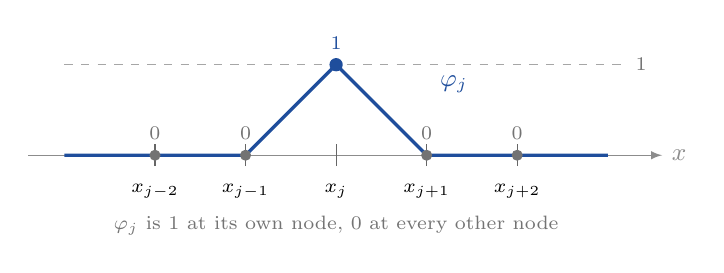
\begin{tikzpicture}[>=latex,x=1.15cm,y=1.15cm]
  \draw[->,black!45] (-0.4,0) -- (6.6,0) node[right,font=\small]{$x$};
  \draw[dashed,black!35] (0,1) -- (6.2,1) node[right,font=\scriptsize,black!55]{$1$};
  % the hat
  \draw[very thick,MathC] (0,0) -- (1,0) -- (2,0) -- (3,1) -- (4,0) -- (5,0) -- (6,0);
  % nodes
  \foreach \x/\lab in {1/{x_{j-2}},2/{x_{j-1}},3/{x_{j}},4/{x_{j+1}},5/{x_{j+2}}}{
    \draw[black!60] (\x,-0.12) -- (\x,0.12);
    \node[below=3pt,font=\scriptsize] at (\x,-0.12) {$\lab$};}
  % the delta values
  \foreach \x in {1,2,4,5}{\fill[black!55] (\x,0) circle (2pt);
    \node[font=\scriptsize,black!55,above=2pt] at (\x,0) {$0$};}
  \fill[MathC] (3,1) circle (2.4pt);
  \node[font=\scriptsize,text=MathC,above=2pt] at (3,1) {$1$};
  \node[font=\small,text=MathC] at (4.3,0.78) {$\varphi_{j}$};
  \node[font=\scriptsize,black!55,align=center] at (3,-0.78)
    {$\varphi_{j}$ is $1$ at its own node, $0$ at every other node};
\end{tikzpicture}
\end{center}

\noindent
\textbf{Between the nodes, the surrounding nodes share the value.} The nodal
condition \eqref{eq:globaldelta} pins $\varphi_{j}$ down only \emph{at} the
nodes. At a point strictly inside an element more than one basis function is
non-zero, and their values sum to one. On the element $[x_{j},x_{j+1}]$ of
width $h$ exactly two hats survive,
\begin{equation}\label{eq:1dpou}
  \varphi_{j}(x)=\frac{x_{j+1}-x}{h},
  \qquad
  \varphi_{j+1}(x)=\frac{x-x_{j}}{h},
  \qquad\text{so}\qquad
  \varphi_{j}(x)+\varphi_{j+1}(x)=1 ,
\end{equation}
the \textbf{partition of unity}.

\begin{center}
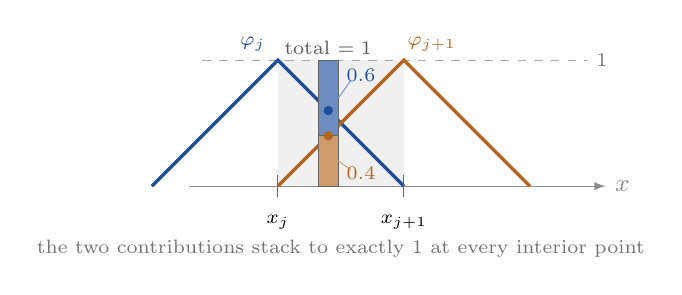
\begin{tikzpicture}[>=latex,x=1.6cm,y=1.6cm]
  \fill[black!6] (3,0) rectangle (4,1);
  \draw[->,black!45] (2.3,0) -- (5.6,0) node[right,font=\small]{$x$};
  \draw[dashed,black!35] (2.4,1) -- (5.45,1) node[right,font=\scriptsize,black!55]{$1$};
  % the two hats
  \draw[very thick,MathC] (2,0) -- (3,1) -- (4,0);
  \draw[very thick,EngC]  (3,0) -- (4,1) -- (5,0);
  \node[font=\scriptsize,text=MathC] at (2.80,1.13) {$\varphi_{j}$};
  \node[font=\scriptsize,text=EngC]  at (4.22,1.13) {$\varphi_{j+1}$};
  % the two contributions at one sample point, stacked
  \fill[EngC!65]  (3.32,0)   rectangle (3.48,0.4);
  \fill[MathC!65] (3.32,0.4) rectangle (3.48,1.0);
  \draw[black!60,thin] (3.32,0) rectangle (3.48,1.0);
  \draw[black!60,thin] (3.32,0.4) -- (3.48,0.4);
  \fill[MathC] (3.4,0.6) circle (1.7pt);
  \fill[EngC]  (3.4,0.4) circle (1.7pt);
  \draw[MathC!55,thin] (3.48,0.70) -- (3.58,0.84);
  \draw[EngC!55,thin]  (3.48,0.20) -- (3.58,0.13);
  \node[font=\scriptsize,text=MathC] at (3.66,0.88) {$0.6$};
  \node[font=\scriptsize,text=EngC]  at (3.66,0.10) {$0.4$};
  \node[font=\scriptsize,black!65] at (3.40,1.10) {total $=1$};
  % nodes
  \foreach \x/\lab in {3/{x_{j}},4/{x_{j+1}}}{
    \draw[black!60] (\x,-0.09) -- (\x,0.09);
    \node[below=3pt,font=\scriptsize] at (\x,-0.09) {$\lab$};}
  \node[font=\scriptsize,black!55] at (3.5,-0.50)
    {the two contributions stack to exactly $1$ at every interior point};
\end{tikzpicture}
\end{center}

\noindent
So $u_{h}(x)=\xi_{j}\varphi_{j}(x)+\xi_{j+1}\varphi_{j+1}(x)$ is a weighted
average of the two nodal values whose weights sum to one: between nodes $u_{h}$
is the straight line joining them, and it can never leave the range of its own
nodal values. The Q4 element behaves identically with four contributions
instead of two --- that is \eqref{eq:pou}.

\medskip
{\small\color{black!60}The identity holds because the constant function $1$ has
nodal value $1$ at every node and lies in $V_{h}$; since the nodal interpolant
is unique, $\sum_{j}\varphi_{j}\equiv1$. The sum must run over \emph{all}
nodes, boundary ones included --- after the constrained boundary functions are
dropped, the identity survives only away from $\partial\Omega$.}

\medskip
\noindent
\textbf{In 2D it is the same statement}, now on a quadrilateral mesh. Below,
the value of $\varphi_{j}$ is written at every node; its support (shaded) is
the four elements touching node $j$:

\begin{center}
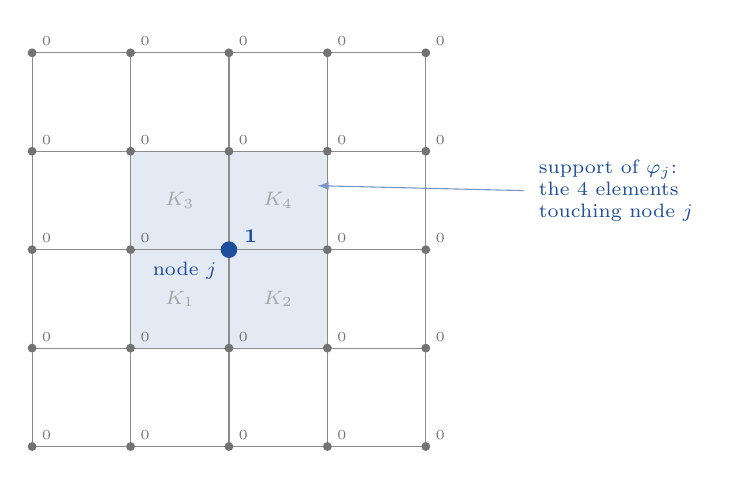
\begin{tikzpicture}[>=latex,x=1.25cm,y=1.25cm]
  % support of phi_j
  \fill[MathC!12] (1,1) rectangle (3,3);
  % mesh
  \foreach \k in {0,1,2,3,4}{
    \draw[black!45] (0,\k) -- (4,\k);
    \draw[black!45] (\k,0) -- (\k,4);}
  % element labels (a couple, to show elements exist)
  \node[font=\scriptsize,black!35] at (1.5,1.5) {$K_{1}$};
  \node[font=\scriptsize,black!35] at (2.5,1.5) {$K_{2}$};
  \node[font=\scriptsize,black!35] at (1.5,2.5) {$K_{3}$};
  \node[font=\scriptsize,black!35] at (2.5,2.5) {$K_{4}$};
  % nodal values -- every node except node j
  \foreach \x/\y in {0/0, 1/0, 2/0, 3/0, 4/0, 0/1, 1/1, 2/1, 3/1, 4/1, 0/2, 1/2, 3/2, 4/2, 0/3, 1/3, 2/3, 3/3, 4/3, 0/4, 1/4, 2/4, 3/4, 4/4}{
      \fill[black!55] (\x,\y) circle (1.6pt);
      \node[font=\tiny,black!55,above right=-1pt and 0pt] at (\x,\y) {$0$};}
  % node j
  \fill[MathC] (2,2) circle (3pt);
  \node[font=\scriptsize,text=MathC,above right=-1pt and 2pt] at (2,2) {$\bm{1}$};
  \node[font=\scriptsize,text=MathC,below left=1pt and 1pt] at (2,2) {node $j$};
  % support callout
  \draw[->,MathC!60] (5.0,2.6) -- (2.9,2.65);
  \node[font=\scriptsize,text=MathC,align=left,right] at (5.05,2.6)
    {support of $\varphi_{j}$:\\ the $4$ elements\\ touching node $j$};
\end{tikzpicture}
\end{center}

\noindent
Both sketches say \eqref{eq:globaldelta} and nothing else. Note what is
\emph{already} present in them: elements ($K_{1},\dots,K_{4}$ and all the
others), nodes, and $\varphi_{j}$ as a function of the real coordinates. Note
what is absent: any mention of $r$, $s$, or a reference square. Those arrive in
Step 3, and only as a computational convenience.

% ------------------------------------------------------------------
\subsection*{Step 2 --- restrict to one element}

Fix one element $K$. Two things happen:
\begin{steps}
\item By \S2, $\varphi_{j}\big|_{K}$ is a \textbf{bilinear polynomial}
      $\alpha+\beta x+\gamma y+\delta xy$.
\item Of the $M$ global basis functions, \textbf{only four are not identically
      zero on $K$} --- those belonging to $K$'s own four corners. Every other
      node lies outside $K$, and its $\varphi$ has already fallen to zero
      there.
\end{steps}
Write that out. Let the four corners of $K$ be the global nodes
$j_{1},j_{2},j_{3},j_{4}$. Restricting the global sum \eqref{eq:uh} to $K$ and
separating those four terms from the rest:
\begin{equation}\label{eq:restrict}
  u_{h}\big|_{K}
  \;=\;\sum_{i=1}^{M}\xi_{i}\,\varphi_{i}\big|_{K}
  \;=\;\underbrace{\xi_{j_{1}}\varphi_{j_{1}}\big|_{K}
       +\xi_{j_{2}}\varphi_{j_{2}}\big|_{K}
       +\xi_{j_{3}}\varphi_{j_{3}}\big|_{K}
       +\xi_{j_{4}}\varphi_{j_{4}}\big|_{K}}
       _{\text{the four corners of }K}
  \;+\!\!\!\sum_{\substack{i=1\\ i\neq j_{1},j_{2},j_{3},j_{4}}}^{M}\!\!\!
       \xi_{i}\underbrace{\varphi_{i}\big|_{K}}_{\equiv\,0} .
\end{equation}
Every term in the second sum vanishes identically on $K$: node $i$ is not a
corner of $K$, so $K$ lies outside the support of $\varphi_{i}$. What is left
is four terms,
\begin{equation}\label{eq:fourterms}
  \boxed{\;u_{h}\big|_{K}
   =\sum_{a=1}^{4}\xi_{j_{a}}\,\varphi_{j_{a}}\big|_{K}\;}
\end{equation}
so we need only four polynomials per element, not $M$.

\medskip
{\small\color{black!60}Concretely, in the mesh drawn above there are $M=25$
nodes, so \eqref{eq:uh} carries $25$ terms. On the element $K_{1}$, $21$ of
them are identically zero and $4$ survive. That ratio is what makes the method
cheap --- and it is why $\bm{A}$ is sparse.}

% ------------------------------------------------------------------
\subsection*{Step 3 --- map $K$ to a fixed square}

Each element has a different size and position, so $\varphi_{j}\big|_{K}$ is a
\emph{different} polynomial in $x,y$ on every element. Rather than redo that
algebra for each one, map every element onto a single \textbf{reference
square} and do the work once:

\begin{center}
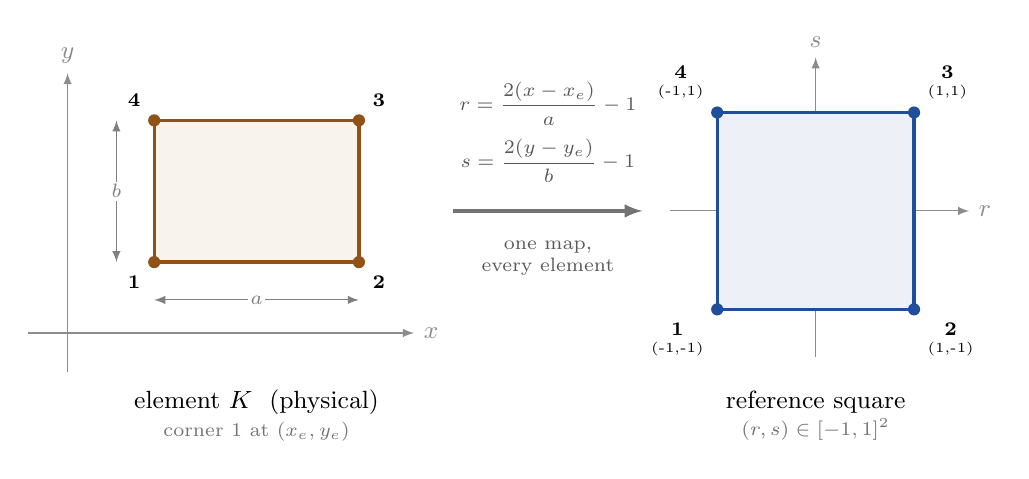
\begin{tikzpicture}[>=latex,x=1cm,y=1cm]
  % ---------------- physical element ----------------
  \begin{scope}
    \draw[->,black!45] (-0.5,0) -- (4.4,0) node[right,font=\small]{$x$};
    \draw[->,black!45] (0,-0.5) -- (0,3.3) node[above,font=\small]{$y$};
    \fill[EngC!8] (1.1,0.9) rectangle (3.7,2.7);
    \draw[very thick,EngC!80!black] (1.1,0.9) rectangle (3.7,2.7);
    \foreach \x/\y/\n/\pos in {1.1/0.9/1/{below left}, 3.7/0.9/2/{below right},
                               3.7/2.7/3/{above right}, 1.1/2.7/4/{above left}}{
      \fill[EngC!80!black] (\x,\y) circle (2.2pt);
      \node[font=\scriptsize,\pos=2pt] at (\x,\y) {\textbf{\n}};}
    \draw[<->,black!50] (1.1,0.42) -- (3.7,0.42)
      node[midway,fill=white,inner sep=1pt,font=\scriptsize]{$a$};
    \draw[<->,black!50] (0.62,0.9) -- (0.62,2.7)
      node[midway,fill=white,inner sep=1pt,font=\scriptsize]{$b$};
    \node[font=\small,align=center] at (2.4,-1.05)
      {element $K$ \ (physical)\\[-1pt]
       {\scriptsize\color{black!55}corner 1 at $(x_{e},y_{e})$}};
  \end{scope}
  % ---------------- the map ----------------
  \draw[->,very thick,black!55] (4.9,1.55) -- (7.3,1.55);
  \node[align=center,font=\scriptsize,black!65] at (6.1,2.55)
    {$r=\dfrac{2(x-x_{e})}{a}-1$\\[4pt] $s=\dfrac{2(y-y_{e})}{b}-1$};
  \node[align=center,font=\scriptsize,black!65] at (6.1,0.95)
    {one map,\\ every element};
  % ---------------- reference square ----------------
  \begin{scope}[xshift=9.5cm,yshift=1.55cm]
    \draw[->,black!45] (-1.85,0) -- (1.95,0) node[right,font=\small]{$r$};
    \draw[->,black!45] (0,-1.85) -- (0,1.95) node[above,font=\small]{$s$};
    \fill[MathC!8] (-1.25,-1.25) rectangle (1.25,1.25);
    \draw[very thick,MathC] (-1.25,-1.25) rectangle (1.25,1.25);
    \foreach \x/\y/\n/\c/\pos in {-1.25/-1.25/1/{(-1,-1)}/{below left},
                                   1.25/-1.25/2/{(1,-1)}/{below right},
                                   1.25/1.25/3/{(1,1)}/{above right},
                                  -1.25/1.25/4/{(-1,1)}/{above left}}{
      \fill[MathC] (\x,\y) circle (2.2pt);
      \node[font=\scriptsize,\pos=2pt,align=center] at (\x,\y)
        {\textbf{\n}\\[-2pt]{\tiny\c}};}
    \node[font=\small,align=center] at (0,-2.60)
      {reference square\\[-1pt]{\scriptsize\color{black!55}$(r,s)\in[-1,1]^{2}$}};
  \end{scope}
\end{tikzpicture}
\end{center}

\noindent
Corner $1$ goes to $(-1,-1)$, corner $2$ to $(1,-1)$, corner $3$ to $(1,1)$,
corner $4$ to $(-1,1)$. The numbering is \emph{local} --- $1,2,3,4$
counter-clockwise from the lower-left corner \emph{of that element}, which is a
different global node in each element.

% ------------------------------------------------------------------
\subsubsection*{Why bother with $(r,s)$ at all?}

Because a real mesh contains elements of many sizes, positions and shapes, and
the \emph{same} local shape function looks different on each one.
Figure~\ref{fig:why} shows four of them.

\begin{center}
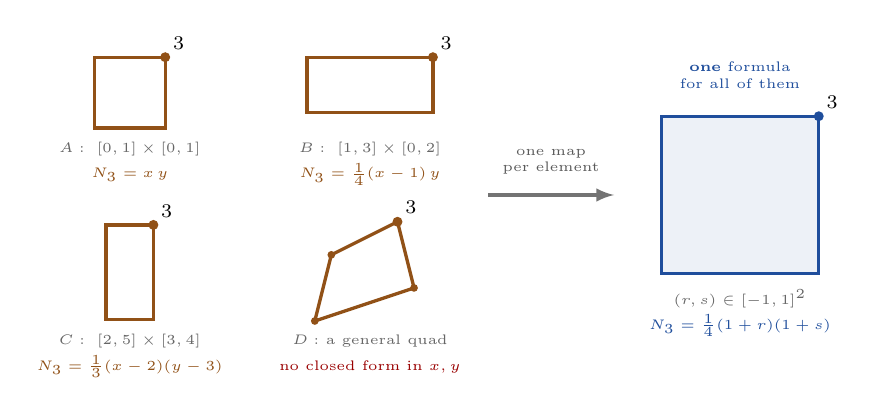
\begin{tikzpicture}[>=latex,x=1cm,y=1cm]
  % ---- four physical elements, each with its own size/position/shape ----
  \begin{scope}
    % A : unit square
    \draw[very thick,EngC!80!black] (0.25,2.95) rectangle (1.15,3.85);
    \fill[EngC!80!black] (1.15,3.85) circle (1.8pt);
    \node[font=\scriptsize,above right=-1pt] at (1.15,3.85) {$3$};
    \node[font=\tiny,black!60] at (0.70,2.68) {$A:\ [0,1]\times[0,1]$};
    \node[font=\tiny,text=EngC!80!black] at (0.70,2.36) {$N_{3}=x\,y$};
    % B : wide rectangle
    \draw[very thick,EngC!80!black] (2.95,3.15) rectangle (4.55,3.85);
    \fill[EngC!80!black] (4.55,3.85) circle (1.8pt);
    \node[font=\scriptsize,above right=-1pt] at (4.55,3.85) {$3$};
    \node[font=\tiny,black!60] at (3.75,2.68) {$B:\ [1,3]\times[0,2]$};
    \node[font=\tiny,text=EngC!80!black] at (3.75,2.36) {$N_{3}=\tfrac14(x-1)\,y$};
    % C : tall rectangle
    \draw[very thick,EngC!80!black] (0.40,0.52) rectangle (1.00,1.72);
    \fill[EngC!80!black] (1.00,1.72) circle (1.8pt);
    \node[font=\scriptsize,above right=-1pt] at (1.00,1.72) {$3$};
    \node[font=\tiny,black!60] at (0.70,0.24) {$C:\ [2,5]\times[3,4]$};
    \node[font=\tiny,text=EngC!80!black] at (0.70,-0.08) {$N_{3}=\tfrac13(x-2)(y-3)$};
    % D : distorted quad
    \draw[very thick,EngC!80!black] (3.05,0.50) -- (4.31,0.92) -- (4.10,1.76) -- (3.26,1.34) -- cycle;
    \foreach \px/\py in {3.05/0.50, 4.31/0.92, 3.26/1.34}{
      \fill[EngC!80!black] (\px,\py) circle (1.4pt);}
    \fill[EngC!80!black] (4.10,1.76) circle (1.8pt);
    \node[font=\scriptsize,above right=-1pt] at (4.10,1.76) {$3$};
    \node[font=\tiny,black!60] at (3.75,0.24) {$D:$ a general quad};
    \node[font=\tiny,text=red!60!black] at (3.75,-0.08) {no closed form in $x,y$};
  \end{scope}
  % ---- the map ----
  \draw[->,very thick,black!55] (5.25,2.10) -- (6.85,2.10);
  \node[font=\tiny,black!65,align=center] at (6.05,2.52) {one map\\ per element};
  % ---- the single reference square ----
  \begin{scope}[xshift=8.45cm,yshift=2.10cm]
    \fill[MathC!8] (-1.0,-1.0) rectangle (1.0,1.0);
    \draw[very thick,MathC] (-1.0,-1.0) rectangle (1.0,1.0);
    \fill[MathC] (1.0,1.0) circle (1.8pt);
    \node[font=\scriptsize,above right=-1pt] at (1.0,1.0) {$3$};
    \node[font=\tiny,black!60] at (0,-1.32) {$(r,s)\in[-1,1]^{2}$};
    \node[font=\tiny,text=MathC] at (0,-1.66) {$N_{3}=\tfrac14(1+r)(1+s)$};
    \node[font=\tiny,text=MathC,align=center] at (0,1.52) {\textbf{one} formula\\ for all of them};
  \end{scope}
\end{tikzpicture}
\captionof{figure}{The same local shape function --- the one that is $1$ at
corner $3$ and $0$ at the other three --- on four different elements. In $x,y$
it is a different polynomial every time, and on the distorted quad $D$ there is
no convenient closed form at all. Mapped to the reference square it is a single
formula, identical for every element in the mesh.}
\label{fig:why}
\end{center}

\noindent
\textbf{The numbers.} Fix one point of the reference square, say
$(r,s)=(0.5,0.5)$, and ask: \emph{how much does node~$3$ contribute there?}
The answer is $N_{3}(0.5,0.5)=\tfrac14(1.5)(1.5)=0.5625$. That one reference
point sits at a \emph{different physical place} $(x,y)$ in each element A, B, C, D, and in
$x,y$ it is evaluated by a \emph{different formula} in each --- yet every one
returns the same share.

\medskip
\noindent
\textbf{The other three make up the rest.} Node~$3$ does not act alone: at the
same point
\begin{equation}\label{eq:shares}
  \underbrace{N_{3}(0.5,0.5)=0.5625}_{\text{node }3}
  \;+\;\underbrace{N_{1}+N_{2}+N_{4}=0.0625+0.1875+0.1875=0.4375}
       _{\text{the other three nodes}}
  \;=0.5625+0.4375=\;1 ,
\end{equation}
which is the partition of unity \eqref{eq:pou} again, now read as a statement
about \emph{shares}: the four nodes divide the point between them, and the
division is the same whether it is described in $(r,s)$ or in $x,y$.

\medskip
\noindent
\textbf{The irony in row $D$.} For $D$ we cannot write down equations for
$N_{1}(x,y)$, $N_{2}(x,y)$, $N_{3}(x,y)$ or $N_{4}(x,y)$ \emph{at all} ---
not one of the four has a closed form in physical coordinates. And suppose we
could: each would be particular to that one element, so a mesh of $10{,}000$
elements would carry
\[
  4\ \text{shape functions}\times10{,}000\ \text{elements}
  \;=\;40{,}000\ \text{formulas},
\]
against exactly $4$ in $(r,s)$.

\medskip
\noindent
\textbf{And it is exactly what Gauss quadrature needs.} Quadrature rules are
not derived per problem --- they are \emph{tabulated}, once, on the standard
interval $[-1,1]$. The $n$-point Gauss--Legendre rule supplies abscissae
$r_{q}$ and weights $w_{q}$ with
\begin{equation}\label{eq:gauss1d}
  \int_{-1}^{1}g(r)\,\mathrm{d}r\;\approx\;\sum_{q=1}^{n}w_{q}\,g(r_{q}),
  \qquad\text{exact for polynomials of degree}\le 2n-1 .
\end{equation}
Because the reference element \emph{is} $[-1,1]^{2}$, those tabulated numbers
apply unchanged to every element in the mesh. Taking the product rule in two
dimensions and inserting the Jacobian,
\begin{equation}\label{eq:gauss2d}
  \iint_{K}f\dOm
  =\int_{-1}^{1}\!\!\int_{-1}^{1}f\bigl(x(r,s),y(r,s)\bigr)\,|J|\,
    \mathrm{d}r\,\mathrm{d}s
  \;\approx\;\sum_{q}w_{q}\,f\bigl(x(r_{q},s_{q}),y(r_{q},s_{q})\bigr)\,
    \bigl|J(r_{q},s_{q})\bigr| .
\end{equation}
For the Q4 element the $2\times2$ rule --- four points at
$(r,s)=(\pm\tfrac{1}{\sqrt3},\pm\tfrac{1}{\sqrt3})$, all four weights equal to
$1$ --- is enough, and \emph{on a rectangle it is exact}: evaluating
\eqref{eq:keint} that way reproduces \eqref{eq:kesq} to machine precision,
because the integrand is degree~$2$ in each variable separately while the rule
is exact through degree~$3$.

\medskip
\noindent
\textbf{Where that degree~$2$ comes from --- in the $\bm{B}$-matrix form you
already use.} Write the Q4 element stiffness as it appears in solid mechanics,
\begin{equation}\label{eq:keBDB}
  \bm{k}^{e}=\underbrace{\int_{\Omega^{e}}
             \bm{B}^{T}\!(x,y)\,\bm{D}\,\bm{B}(x,y)\dOm}
             _{\text{over the physical element}}
           =\underbrace{\int_{-1}^{1}\!\!\int_{-1}^{1}
             \bm{B}^{T}\!(r,s)\,\bm{D}\,\bm{B}(r,s)\,
             \bigl|J(r,s)\bigr|\,\mathrm{d}r\,\mathrm{d}s}
             _{\text{over the reference square}} ,
\end{equation}
with $\bm{d}=[u_{1}\,v_{1}\,u_{2}\,v_{2}\,u_{3}\,v_{3}\,u_{4}\,v_{4}]^{T}$,
$\bm{\varepsilon}=\bm{B}\bm{d}$ and, for plane stress,
$\bm{D}=\frac{E}{1-\nu^{2}}
\left[\begin{smallmatrix}1&\nu&0\\ \nu&1&0\\ 0&0&\frac{1-\nu}{2}\end{smallmatrix}\right]$.
The strain--displacement matrix is $\bm{B}=\partial\bm{N}$:
\begin{equation}\label{eq:Bmat}
  \bm{B}=
  \begin{bmatrix}
    N_{1,x} & 0       & N_{2,x} & 0       & N_{3,x} & 0       & N_{4,x} & 0\\
    0       & N_{1,y} & 0       & N_{2,y} & 0       & N_{3,y} & 0       & N_{4,y}\\
    N_{1,y} & N_{1,x} & N_{2,y} & N_{2,x} & N_{3,y} & N_{3,x} & N_{4,y} & N_{4,x}
  \end{bmatrix}.
\end{equation}

\medskip
\noindent
\textbf{One caution on the notation in \eqref{eq:keBDB}.} Writing
$\bm{B}(r,s)$ does \emph{not} mean its entries are derivatives with respect to
$r$ and $s$. They are still $\partial N_{a}/\partial x$ and
$\partial N_{a}/\partial y$ --- derivatives with respect to the \emph{physical}
coordinates, as \eqref{eq:Bmat} says. The argument $(r,s)$ only records
\emph{where} they are evaluated. The two are connected by the chain rule
\eqref{eq:jac}: the code forms $\partial N_{a}/\partial r$ and
$\partial N_{a}/\partial s$ first because those are the easy ones, then
multiplies by $J^{-1}$ to get the $x,y$ derivatives that $\bm{B}$ actually
holds.

\medskip
\noindent
\textbf{The summation form --- what the code actually loops over.} The
integral in \eqref{eq:keBDB} is never evaluated symbolically. Replacing it by
the Gauss sum \eqref{eq:gauss2d} gives the matrix form
\begin{equation}\label{eq:kesum}
  \boxed{\;
  \bm{k}^{e}=\sum_{q=1}^{n_{gp}} w_{q}\,
     \bm{B}^{T}(r_{q},s_{q})\,\bm{D}\,\bm{B}(r_{q},s_{q})\,
     \bigl|J(r_{q},s_{q})\bigr|\;}
\end{equation}
and, written entry by entry, exactly the nested loops a program runs:
\begin{equation}\label{eq:kesumij}
  k^{e}_{ij}=\sum_{q=1}^{n_{gp}}\;w_{q}\,\bigl|J_{q}\bigr|
     \sum_{k=1}^{3}\sum_{l=1}^{3}
     B_{ki}(r_{q},s_{q})\;D_{kl}\;B_{lj}(r_{q},s_{q}),
  \qquad i,j=1,\dots,8 .
\end{equation}
For the Q4 element $n_{gp}=4$, with
$(r_{q},s_{q})=(\pm\tfrac{1}{\sqrt3},\pm\tfrac{1}{\sqrt3})$ and $w_{q}=1$.

\medskip
\noindent
In code that is four loops --- over Gauss points, then over the $8\times8$
entries, with the $3\times3$ material contraction inside:

\begin{quote}\ttfamily\small
ke = zeros(8,8)\\
for q in 1..ngp:\qquad\textrm{\# Gauss points}\\
\hspace*{1.2em}r, s, w = gp[q]\\
\hspace*{1.2em}dNdr, dNds = shape\_derivs(r, s)\qquad\textrm{\# 4 each}\\
\hspace*{1.2em}Jm = [[dNdr$\cdot$x, dNdr$\cdot$y], [dNds$\cdot$x, dNds$\cdot$y]]\qquad\textrm{\# 2x2}\\
\hspace*{1.2em}detJ = det(Jm)\\
\hspace*{1.2em}dNdx, dNdy = solve(Jm, [dNdr; dNds])\qquad\textrm{\# chain rule}\\
\hspace*{1.2em}B = assemble\_B(dNdx, dNdy)\qquad\textrm{\# 3x8, eq.\ \ref{eq:Bmat}}\\
\hspace*{1.2em}ke += w * detJ * B.T @ D @ B
\end{quote}

\noindent
Note the order: the shape-function derivatives are formed in $(r,s)$, the
Jacobian converts them to $x,y$, and only then is $\bm{B}$ built. The element's
geometry enters through \texttt{Jm} alone --- \texttt{shape\_derivs} is the
same four formulas for every element in the mesh.

\medskip
\noindent
Now read the degrees straight off \eqref{eq:keBDB}:
\begin{steps}
\item \textbf{Every entry of $\bm{B}$ is a \emph{first derivative} of a shape
      function.} $N_{a}$ is degree $1$ in $r$ and $1$ in $s$; differentiating
      removes one, so each $N_{a,x}$ or $N_{a,y}$ is degree
      $\le1$ in $r$ and $\le1$ in $s$.
\item \textbf{$\bm{D}$ contributes no $r,s$ dependence} --- for a homogeneous
      linear-elastic material it is a matrix of constants.
\item \textbf{So $\bm{B}^{T}\bm{D}\bm{B}$ is $\bm{B}$ \emph{times} $\bm{B}$.}
      Each entry is
      $\sum_{k,l}B_{ki}D_{kl}B_{lj}$ --- a sum of \emph{products of two}
      $\bm{B}$ entries, \ie\ two first derivatives multiplied together. One
      derivative is degree $\le1$ per variable; two multiplied give
      degree~$\le2$ per variable.
\end{steps}

\noindent
That is what ``the integrand multiplies two derivatives'' meant:
it is the $\bm{B}^{T}(\cdots)\bm{B}$ sandwich. Checked symbolically on the
unit square: every entry of $\bm{B}$ has degree $\le1$ in $r$ and in $s$, and
every entry of $\bm{B}^{T}\bm{D}\bm{B}$ has degree exactly $2$ in $r$ and $2$
in $s$ --- so the $2$-point rule, exact through degree~$3$, covers it.

\medskip
\noindent
The Poisson problem of this note is the same structure with one unknown per
node instead of two: $\bm{B}$ collapses to the $2\times4$ gradient matrix
$\left[\begin{smallmatrix}N_{1,x}&N_{2,x}&N_{3,x}&N_{4,x}\\
N_{1,y}&N_{2,y}&N_{3,y}&N_{4,y}\end{smallmatrix}\right]$ and
$\bm{D}=\bm{I}$, so $\bm{B}^{T}\bm{D}\bm{B}$ reduces entry-by-entry to
$\grad N_{a}\cdot\grad N_{b}=N_{a,x}N_{b,x}+N_{a,y}N_{b,y}$ --- the integrand
in \eqref{eq:keint}. Two derivatives multiplied, again.

\medskip
\noindent
\textbf{On a distorted element it is no longer exact.} Everything above
assumed the integrand is a \emph{polynomial}. Here is where that assumption
comes from, and where it breaks.

\medskip
\noindent
\textbf{Step 1 --- the chain rule divides by $\det J$.} The easy derivatives
are $\partial N_{a}/\partial r$ and $\partial N_{a}/\partial s$. The ones
$\bm{B}$ needs are $\partial N_{a}/\partial x$ and $\partial N_{a}/\partial y$,
and they are obtained by \emph{inverting} the Jacobian:
\begin{equation}\label{eq:chaininv}
  \underbrace{\begin{bmatrix}
    N_{1,x} & N_{2,x} & N_{3,x} & N_{4,x}\\
    N_{1,y} & N_{2,y} & N_{3,y} & N_{4,y}
  \end{bmatrix}}_{\text{the }x,y\text{ derivatives, }2\times4}
  =\bm{J}^{-1}
  \underbrace{\begin{bmatrix}
    N_{1,r} & N_{2,r} & N_{3,r} & N_{4,r}\\
    N_{1,s} & N_{2,s} & N_{3,s} & N_{4,s}
  \end{bmatrix}}_{\text{the easy ones, }2\times4},
  \qquad
  \bm{J}^{-1}=\frac{1}{\det\bm{J}}\,\mathrm{adj}\,\bm{J} .
\end{equation}
Those eight numbers are precisely what fills the element strain--displacement
matrix: row~$1$ of \eqref{eq:chaininv} supplies the top row of $\bm{B}^{e}$,
row~$2$ supplies the middle row, and the two interleaved give the shear row,
\begin{equation}\label{eq:Befilled}
  \bm{B}^{e}=
  \begin{bmatrix}
    N_{1,x} & 0       & N_{2,x} & 0       & N_{3,x} & 0       & N_{4,x} & 0\\
    0       & N_{1,y} & 0       & N_{2,y} & 0       & N_{3,y} & 0       & N_{4,y}\\
    N_{1,y} & N_{1,x} & N_{2,y} & N_{2,x} & N_{3,y} & N_{3,x} & N_{4,y} & N_{4,x}
  \end{bmatrix}
  \qquad\text{(this is \eqref{eq:Bmat})} .
\end{equation}
Since every $N_{a,x}$ and $N_{a,y}$ came out of \eqref{eq:chaininv} carrying
the factor $1/\det\bm{J}$ from $\bm{J}^{-1}$, \textbf{every entry of
$\bm{B}^{e}$ carries it too}.

\medskip
\noindent
\textbf{Step 2 --- count the factors in the integrand.} From
\eqref{eq:keBDB} the integrand is $\bm{B}^{T}\bm{D}\bm{B}\,|J|$:
\[
  \underbrace{\frac{1}{\det\bm{J}}}_{\text{from the first }\bm{B}}\times
  \underbrace{\frac{1}{\det\bm{J}}}_{\text{from the second }\bm{B}}\times
  \underbrace{\det\bm{J}}_{\text{from }\dOm}
  \;=\;\frac{1}{\det\bm{J}} .
\]
One factor cancels, \textbf{one survives in the denominator}.

\medskip
\noindent
\textbf{Step 3 --- so it depends entirely on whether $\det\bm{J}$ is constant.}
First, what $\bm{J}$ actually is. It is the $2\times2$ matrix of derivatives of
the map, and because the map is $x=\sum_{a}N_{a}x_{a}$, $y=\sum_{a}N_{a}y_{a}$,
it is built straight from the nodal coordinates:
\begin{equation}\label{eq:Jdef}
  \bm{J}=
  \begin{bmatrix}
    \dfrac{\partial x}{\partial r} & \dfrac{\partial y}{\partial r}\\[10pt]
    \dfrac{\partial x}{\partial s} & \dfrac{\partial y}{\partial s}
  \end{bmatrix}
  =\begin{bmatrix}
    \sum_{a}N_{a,r}\,x_{a} & \sum_{a}N_{a,r}\,y_{a}\\[4pt]
    \sum_{a}N_{a,s}\,x_{a} & \sum_{a}N_{a,s}\,y_{a}
  \end{bmatrix},
  \qquad
  \det\bm{J}=\frac{\partial x}{\partial r}\frac{\partial y}{\partial s}
            -\frac{\partial y}{\partial r}\frac{\partial x}{\partial s} .
\end{equation}
(That second form is the \texttt{Jm} line of the loop above.) Now put the two
elements through it.

\begin{steps}
\item \textbf{Rectangle} $a\times b$. The map is simply
      $x=x_{e}+\tfrac{a}{2}(r+1)$, $y=y_{e}+\tfrac{b}{2}(s+1)$ --- $x$ depends
      on $r$ alone and $y$ on $s$ alone, so the off-diagonal derivatives
      vanish:
      \[
        \bm{J}=\begin{bmatrix} \tfrac{a}{2} & 0\\[2pt] 0 & \tfrac{b}{2}\end{bmatrix},
        \qquad
        \det\bm{J}=\frac{a}{2}\cdot\frac{b}{2}-0\cdot0=\frac{ab}{4} .
      \]
      \textbf{No $r$, no $s$ anywhere in it} --- $\det\bm{J}$ is a
      \emph{number}, fixed by the element's two side lengths. Dividing a
      polynomial by a number leaves a polynomial, so Gauss is exact.

      \medskip
      \noindent\fbox{\parbox{0.90\linewidth}{\small
      \textbf{Why $ab/4$ and not $ab$?} $\det\bm{J}$ is \emph{not} the area ---
      it is the \textbf{area scaling factor}, the ratio of physical area to
      reference area:
      \[
        \dOm=\mathrm{d}x\,\mathrm{d}y=\det\bm{J}\;\mathrm{d}r\,\mathrm{d}s .
      \]
      The reference square $[-1,1]^{2}$ has area $2\times2=\mathbf{4}$, not
      $1$. So the area is recovered by \emph{integrating}, not by reading:
      \[
        \text{area}=\int_{-1}^{1}\!\!\int_{-1}^{1}\det\bm{J}\,\mathrm{d}r\,\mathrm{d}s
        =\frac{ab}{4}\times4=ab .\ \cmark
      \]
      A second way to see that $\det\bm{J}$ cannot itself be an area: on
      element $D$ it \emph{varies} from $3$ to $4$ across the element,
      and one element has only one area. Its integral is the area, though ---
      $\int\!\!\int\det\bm{J}=14$, exactly $D$'s area by the shoelace formula.}}

\item \textbf{Distorted quad $D$.} Here the map \eqref{eq:fwdD} is
      $x=2+\tfrac32r+\tfrac12s$, $y=\tfrac94-\tfrac14r+\tfrac94s-\tfrac14rs$ ---
      note the $rs$ term, which makes $y$ depend on $r$ as well. So the
      off-diagonal entries do \emph{not} vanish:
      \[
        \bm{J}=\begin{bmatrix}
          \tfrac32 & -\tfrac14-\tfrac{s}{4}\\[3pt]
          \tfrac12 & \tfrac94-\tfrac{r}{4}
        \end{bmatrix},
        \qquad
        \det\bm{J}=\tfrac32\Bigl(\tfrac94-\tfrac{r}{4}\Bigr)-\Bigl(-\tfrac14-\tfrac{s}{4}\Bigr)\Bigl(\tfrac12\Bigr)
        =\tfrac72-\tfrac{3r}{8}+\tfrac{s}{8}.
      \]
      \textbf{Now $r$ and $s$ survive} --- $\det\bm{J}$ is a \emph{function},
      taking a different value at every point of the element. It stays in the
      denominator, and the integrand becomes a \textbf{ratio of polynomials}:
\begin{align}
  \frac{\partial N_{1}}{\partial x}
    &=\frac{r+4s-5}{\,28-3r+s\,}
    \qquad\text{\small(denominator $=8\det\bm{J}$)},\notag\\[4pt]
  \underbrace{\Bigl[\bigl(\tfrac{\partial N_{1}}{\partial x}\bigr)^{2}
             +\bigl(\tfrac{\partial N_{1}}{\partial y}\bigr)^{2}\Bigr]\det\bm{J}}
             _{\text{the } k^{e}_{11}\text{ integrand}}
    &=\frac{(r+4s-5)^{2}+(3r-s-2)^{2}}{8\,(28-3r+s)} .\label{eq:rational}
\end{align}
\end{steps}

\medskip
\noindent\fbox{\parbox{0.955\linewidth}{\small
\textbf{Four Gauss points, four different $\det\bm{J}$ --- what does that
mean?} The $2\times2$ rule puts its points at
$(r,s)=(\pm g,\pm g)$ with $g=1/\sqrt3=0.577350$, all weights $1$. Evaluating
$\det\bm{J}=\tfrac72-\tfrac{3r}{8}+\tfrac{s}{8}$ at each:

\medskip
\centering
\renewcommand{\arraystretch}{1.25}
\begin{tabular}{@{}clccc@{}}
\toprule
$q$ & $(r_{q},s_{q})$ & maps to $(x,y)$ & $\det\bm{J}$ & value\\
\midrule
$1$ & $(-g,-g)$ & $(0.8453,\,1.0120)$ & $\tfrac72+\tfrac{\sqrt3}{12}$ & $3.644338$\\
$2$ & $(+g,-g)$ & $(2.5774,\,0.8900)$ & $\tfrac72-\tfrac{\sqrt3}{6}$  & $3.211325$\\
$3$ & $(+g,+g)$ & $(3.1547,\,3.3214)$ & $\tfrac72-\tfrac{\sqrt3}{12}$ & $3.355662$\\
$4$ & $(-g,+g)$ & $(1.4226,\,3.7767)$ & $\tfrac72+\tfrac{\sqrt3}{6}$  & $3.788675$\\
\bottomrule
\end{tabular}

\medskip
\begin{center}
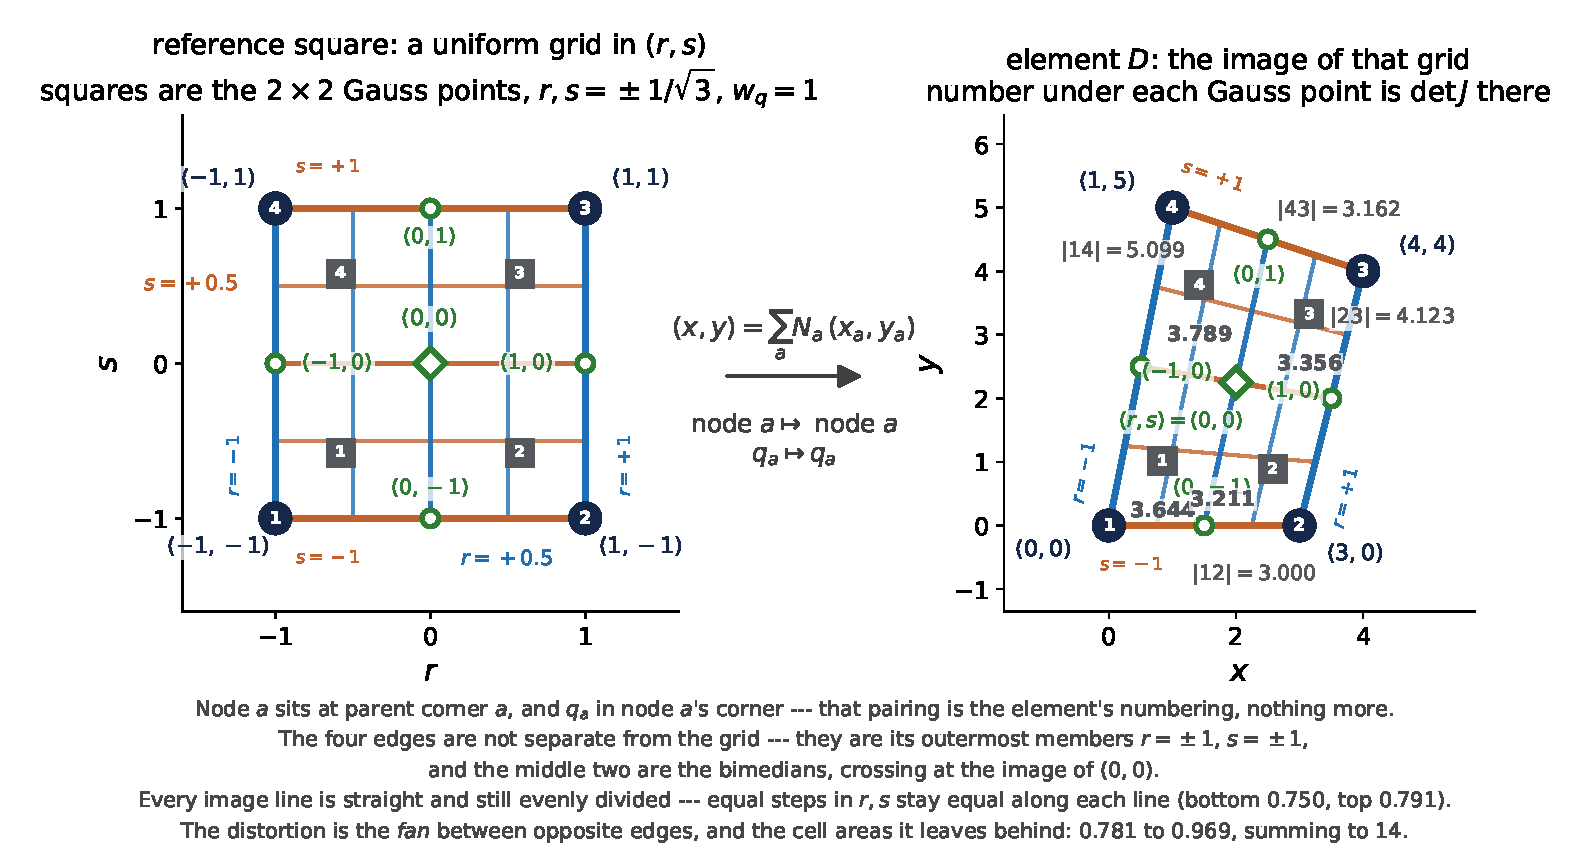
\includegraphics[width=\linewidth]{q4_elemD.pdf}
\captionof{figure}{\textbf{Left:} the reference square. \textbf{Right:} element
$D$, carrying the \emph{same} grid. Blue lines are $r=\text{const}$, orange
lines are $s=\text{const}$, and each edge is labelled with the grid line it
\emph{is}; the two middle members are the bimedians. Every marker carries its
index \emph{inside} it, so node~$a$ and Gauss point $q_{a}$ mean the same thing
in both panels. Green: $(r,s)$-landmarks --- the centre and the four parent
edge midpoints --- and their images. Grey: edge lengths $|ab|$, and
$\det\bm{J}$ under each Gauss point.}
\label{fig:elemD}
\end{center}

\medskip
\raggedright
\textbf{The four parent corners, put through the map.} At a corner three of the
four $N_{a}$ vanish and the fourth is $1$ --- the nodal condition
\eqref{eq:delta} --- so the sum collapses onto a single nodal coordinate:

\medskip
\centering
{\footnotesize
\renewcommand{\arraystretch}{1.3}
\begin{tabular}{@{}ccccl@{}}
\toprule
$(r,s)$ & $(N_{1},N_{2},N_{3},N_{4})$
        & $x=\sum_{a}N_{a}x_{a}$ & $y=\sum_{a}N_{a}y_{a}$ & gives\\
\midrule
$(-1,-1)$ & $(1,0,0,0)$ & $1(0)+0(3)+0(4)+0(1)$ & $1(0)+0(0)+0(4)+0(5)$
          & $(0,0)=$ node $1$\\
$(1,-1)$  & $(0,1,0,0)$ & $0(0)+1(3)+0(4)+0(1)$ & $0(0)+1(0)+0(4)+0(5)$
          & $(3,0)=$ node $2$\\
$(1,1)$   & $(0,0,1,0)$ & $0(0)+0(3)+1(4)+0(1)$ & $0(0)+0(0)+1(4)+0(5)$
          & $(4,4)=$ node $3$\\
$(-1,1)$  & $(0,0,0,1)$ & $0(0)+0(3)+0(4)+1(1)$ & $0(0)+0(0)+0(4)+1(5)$
          & $(1,5)=$ node $4$\\
\bottomrule
\end{tabular}}

\medskip
\raggedright
Reading the same four off the collapsed form \eqref{eq:fwdD} costs no $N$'s at
all: $x=2+\tfrac{3r}{2}+\tfrac{s}{2}$ and
$y=\tfrac94-\tfrac{r}{4}+\tfrac{9s}{4}-\tfrac{rs}{4}$ give, at $(-1,-1)$,
$2-\tfrac32-\tfrac12=0$ and $\tfrac94+\tfrac14-\tfrac94-\tfrac14=0$, and so on
round the element.}}

\medskip
\noindent\fbox{\parbox{0.955\linewidth}{\small
\textbf{What that table is telling you.}

\medskip
\textbf{1. The element passes exactly through its own nodes.} This is the one
place where the map is not an approximation of anything: corner $a$ of the
parent lands \emph{on} node $a$, for any quadrilateral you like, however
distorted. It is \eqref{eq:delta} doing its job in the geometry slot instead of
the unknown slot.

\medskip
\textbf{2. Everywhere else all four are alive, and they are weights.} They sum
to $1$ at every point of the square, \eqref{eq:pou}, so the image is always a
\emph{weighted average} of the four corners --- which is also why it can never
escape the quad. At the centre all four equal $\tfrac14$:
\[
  x(0,0)=\tfrac{0+3+4+1}{4}=2,\qquad
  y(0,0)=\tfrac{0+0+4+5}{4}=\tfrac94 ,
\]
the green diamond in the figure. The corner table is just the extreme case of
this, with the weights $(1,0,0,0)$ instead of $(\tfrac14,\tfrac14,\tfrac14,
\tfrac14)$.

\medskip
\textbf{3. On an edge, two of them die and the other two go linear.} Set
$s=-1$:
\[
  (N_{1},N_{2},N_{3},N_{4})\big|_{s=-1}
  =\bigl(\tfrac{1-r}{2},\ \tfrac{1+r}{2},\ 0,\ 0\bigr).
\]
Nodes $3$ and $4$ drop out completely and the survivors are linear in $r$, so
that edge maps to the \emph{straight} segment from node~$1$ to node~$2$ and the
parent midpoint $(0,-1)$ lands on the physical midpoint $(\tfrac32,0)$ --- the
green ring on the bottom edge. Two consequences worth keeping:
\emph{(i)} the edges of a Q4 are straight even though its interior map is
bilinear --- every $N_{a}$ carries one factor $(1\pm r)$ and one $(1\pm s)$, so
fixing $s=\pm1$ kills two of them outright and strips the $s$ out of the other
two, leaving a map linear in $r$ alone; \emph{(ii)} the image of edge $s=-1$ depends on
nodes $1$ and $2$ \textbf{and nothing else}, so the element on the far side of
that edge --- whatever its own local numbering --- builds the identical
segment from the identical two nodes. That is the conformity of \S2, visible
here as two zeros in a row of the table.

\medskip
\textbf{4. One thing to be careful about.} $(0,0)$ maps to the plain average of
the four corners, $(2,\tfrac94)$. That is the \emph{vertex} centroid, and $D$
has two other equally reasonable ``centres'' --- all three different:
\[
  \underbrace{\bigl(2,\tfrac94\bigr)}_{\text{vertex centroid}=\,(0,0)},\qquad
  \underbrace{\bigl(\tfrac{41}{21},\tfrac{16}{7}\bigr)}_{\text{area centroid}}
   =(1.9524,2.2857),\qquad
  \underbrace{\bigl(\tfrac{15}{7},\tfrac{15}{7}\bigr)}_{\text{diagonals cross}}
   =(2.1429,2.1429).
\]
They coincide for a parallelogram and separate for everything else, so ``the
centre of the element'' is ambiguous unless you say which one you mean. Everything in this
note that gets evaluated at $(r,s)=(0,0)$ --- the map, the crossing point of
the two bimedians, the mean of the four corner Jacobians --- returns the
first.}}

\medskip
\noindent\fbox{\parbox{0.955\linewidth}{\small
\raggedright
\textbf{``Conforming'' --- and the two other things that word is used for.}
``Continuous'' and ``conforming'' are not two words for the same thing, and
that is the whole source of the confusion. They answer different questions.}}

\medskip
\textbf{Two questions, four boxes.}

\medskip
\begin{center}\small
\renewcommand{\arraystretch}{1.4}
\begin{tabular}{@{}l@{\hspace{1.3em}}l@{\hspace{1.3em}}l@{}}
\toprule
the word & the question it answers & where you look\\
\midrule
continuous / discontinuous & is there a \emph{gap} at the shared edge?
  & at the mesh\\
conforming / non-conforming & is that gap \emph{legal} for this equation?
  & at the PDE\\
\bottomrule
\end{tabular}
\captionof{table}{The two independent questions behind the four combinations
of Figure~\ref{fig:fourboxes}. The second one is not a property of the
element: change the PDE and the answer changes without the element moving.}
\label{tab:twoquestions}
\end{center}
\medskip
\textbf{Two PDEs, the same ten steps.} Only one thing differs between the
columns --- how many times you integrate by parts. Everything under that row
is forced by it.

\begin{center}\small
\renewcommand{\arraystretch}{1.4}
\begin{tabular}{@{}l@{\hspace{1.4em}}l@{\hspace{1.4em}}l@{}}
\toprule
 & \textbf{Poisson}, order $2$ & \textbf{Euler--Bernoulli beam}, order $4$\\
\midrule
strong form & $-(k\,u')'=f$ & $(EI\,w'')''=q$\\
integrate by parts & \emph{once} & \emph{twice}\\
weak form
  & $\displaystyle\int k\,u'v'=\int fv$
  & $\displaystyle\int EI\,w''v''=\int qv$\\
derivatives, trial\,/\,test & $1\,/\,1$ & $2\,/\,2$\\
so the space is & $V=H^{1}$ & $V=H^{2}$\\
must be continuous at the edge & $u$ & $w$ \emph{and} $w'$\\
free to jump & $u'$ & $w''$\\
continuity class & $C^{0}$ & $C^{1}$\\
what the two elements share & the value & the value \emph{and} the slope\\
cheapest conforming element & linear Lagrange, $2$ DOF
  & Hermite cubic, $4$ DOF\\
\bottomrule
\end{tabular}
\captionof{table}{The same derivation run on a second- and a fourth-order
problem. How the derivatives split between trial and test function is what
fixes $V$; $V$ fixes the continuity class; and the continuity class fixes
which quantities have to be nodal unknowns.}
\label{tab:twopdes}
\end{center}

\textbf{The pattern.} A PDE of order $2m$ hands $m$ derivatives to the trial
function and $m$ to the test function, so $V=H^{m}$, so the element must be
$C^{m-1}$: everything up to the $(m\!-\!1)$st derivative is shared at the
node, and the $m$th derivative is free to jump. That one sentence generates
both columns.

\medskip
\textbf{One trap: $C^{1}$ does not mean ``quadratic''.} Continuity class and
polynomial degree are independent. A quadratic Lagrange element is still
$C^{0}$ --- the extra mid-side node raises the \emph{degree}, but the element
still shares only \emph{values} with its neighbour, so the slope still jumps
and a beam built from it is still non-conforming. $C^{1}$ comes from making
the slope a \emph{nodal unknown}, which is exactly what the Hermite cubic
does: degree $3$, and $C^{1}$ because $w'$ sits at the node and both elements
read the same one. Raising the degree never buys continuity; changing which
quantities are shared does.

\pagebreak[1]
\begin{center}
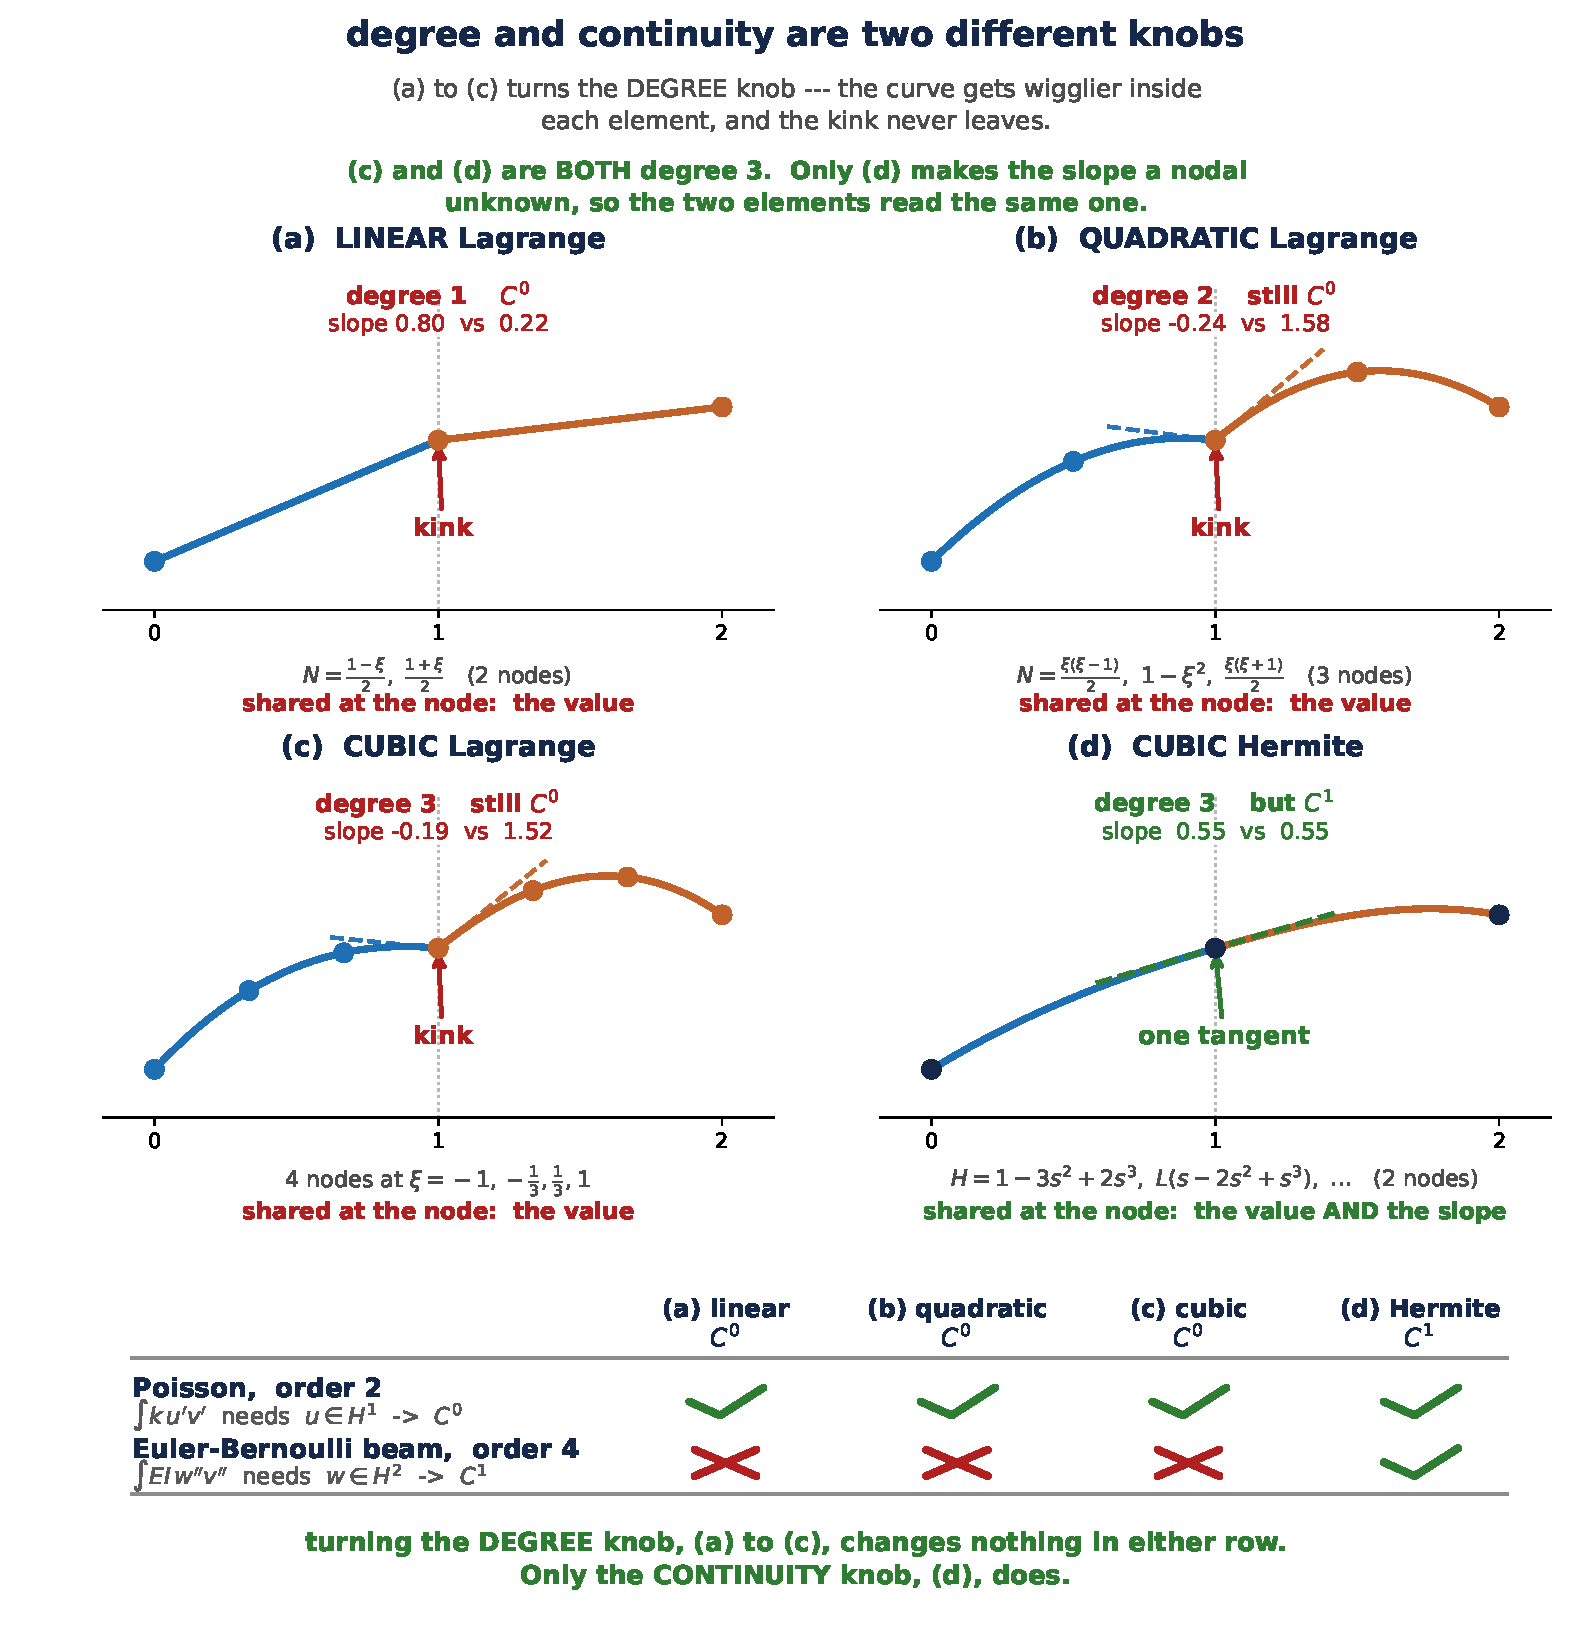
\includegraphics[width=0.96\linewidth]{q4_degree_vs_continuity.pdf}
\captionof{figure}{Degree and continuity are two separate knobs, shown on two
elements joined at $x=1$. \textbf{(a)\,$\to$\,(b)\,$\to$\,(c)} turns the
\emph{degree} knob --- $1$, $2$, $3$ --- and the curve gets wigglier inside
each element while the kink at the joint never leaves: all three are $C^{0}$,
because all three share only the \emph{value} with the neighbour. The dashed
tangents and the printed slopes make the mismatch explicit
($0.80$ vs $0.22$, then $-0.24$ vs $1.58$, then $-0.19$ vs $1.52$).
\textbf{(c) and (d) are both degree $3$} --- the comparison worth staring at.
(d) is $C^{1}$ not because it is a higher polynomial, but because $w'$ was made
a \emph{nodal unknown}, so the two elements read one tangent instead of two.
\textbf{Bottom strip:} the same four elements judged by the two PDEs of
Table~\ref{tab:twopdes}. Poisson asks for $C^{0}$ and every column passes;
the beam asks for $C^{1}$ and only (d) does. Turning the degree knob moves
nothing in either row.}
\label{fig:degvscont}
\end{center}

\medskip
\textbf{Q. What if I use $C^{0}$ linear Lagrange on the Euler--Bernoulli beam
--- is that conforming or non-conforming? look at the pde only. no need to look at the mesh}

\medskip
\textbf{A. Non-conforming --- and not in a useful way. The element has
\emph{zero} bending stiffness.}

\medskip
Follow the arithmetic rather than the definition. A linear $w$ has $w''=0$
inside the element, so the weak-form integrand $EI\,w''v''$ is identically
zero and
\[
  k^{e}=\int_{0}^{L}EI\,w''\,v''\dx
       =\begin{bmatrix}0&0\\[2pt]0&0\end{bmatrix},
  \qquad \operatorname{rank}=0 .
\]
Not nearly singular --- \emph{exactly} the zero matrix. Every nodal
displacement is a zero-energy mode, the assembled $K$ is entirely singular,
and the solver has nothing to invert.

\medskip
The formal reason is that same fact seen from the other side.
Piecewise-linear $C^{0}$ functions are not in $H^{2}$: the slope jumps at
every node, so $w''$ carries a Dirac delta there and $\int(w'')^{2}$ is not
finite. The energy is $0$ inside the elements and undefined at the nodes, so
$V_{h}\not\subset V$.\\

 
So the same element on the same mesh --- $C^{0}$ linear Lagrange --- is
\emph{conforming} for Poisson and \emph{non-conforming} for the beam. Nothing
about the element changed; the equation did. That is the whole distinction.

\medskip
\textbf{What the weak form does and does not settle.} Counting the derivatives
in the weak form gives you the \emph{requirement}: order $2m$ needs $C^{m-1}$,
and you can read that off without ever seeing a mesh. It does not give you the
\emph{verdict}. Whether a particular element meets that bar is a question
about the element --- which quantities does it actually share with its
neighbour? Two steps, two different objects, which is precisely the two rows
of Table~\ref{tab:twoquestions}. Crouzeix--Raviart is the reminder: a
second-order problem asks only for $C^{0}$, and that element still fails to
deliver it, being continuous at edge midpoints alone.

\medskip
\textbf{Q. Is $C^{1}$ possible at degree $1$ or $2$? And could I use it on a
beam, or is it only $H^{1}$?}

\medskip
\textbf{A. As a \emph{nodal element}, no --- the minimum is cubic. As a
\emph{spline}, yes --- and it does carry a beam.} The phrase ``$C^{1}$
quadratic'' means two different things, and they have opposite answers.

\medskip
\textbf{As a nodal element: count coefficients against conditions.} $C^{1}$
means matching the value \emph{and} the slope at \emph{both} ends: four
demands.

\begin{center}\small
\renewcommand{\arraystretch}{1.3}
\begin{tabular}{@{}l@{\hspace{1.5em}}c@{\hspace{1.5em}}c@{\hspace{1.5em}}l@{}}
\toprule
degree & free coefficients & four conditions? & what you get\\
\midrule
$1$, linear & $2$ & \xmark & the whole mesh collapses to one line\\
$2$, quadratic & $3$ & \xmark & the nodal values are not independent\\
$3$, cubic & $4$ & \cmark & the Hermite beam element\\
\bottomrule
\end{tabular}
\captionof{table}{Why the Hermite element is \emph{cubic}. It is not a design
choice --- four conditions need four coefficients.}
\label{tab:c1count}
\end{center}

For the quadratic the system has no solution: impose the first three
conditions and the fourth forces
\[
  w_{2}=w_{1}+\tfrac{L}{2}\bigl(\theta_{1}+\theta_{2}\bigr),
\]
so you cannot hand such an element an arbitrary
$(w_{1},\theta_{1},w_{2},\theta_{2})$. Degree $1$ fails worse, and for a
reason worth picturing: if a piecewise-linear function has a continuous slope
at \emph{every} node, the slope is the same everywhere and the whole mesh is
one straight line --- two degrees of freedom in total, however many elements
you use. The rule behind the table is that $C^{k}$ needs degree $\ge 2k+1$:
$C^{0}\to1$, $C^{1}\to3$, $C^{2}\to5$.

\medskip
\textbf{As a spline: a quadratic \emph{is} $C^{1}$, and it works.} Quadratic
B-splines with simple knots are $C^{1}$ across every knot. Checked on four
elements: the jump in $w'$ at an interior knot is $1.6\times10^{-6}$ (zero),
while the jump in $w''$ is $48$ --- so exactly $C^{1}$, not $C^{2}$. Assembling
the beam stiffness $\int EI\,w''v''\dx$ over that space gives eigenvalues
\[
  0,\quad 0,\quad 50.49,\quad 363.2,\quad 973.5,\quad 1172.8,
\]
rank $4$ of $6$, nullity $2$ --- the two rigid-body modes, exactly as for the
Hermite cubic, and emphatically \emph{not} the zero matrix that $C^{0}$ linear
Lagrange produced above.

\medskip
\textbf{How does that dodge the counting argument?} It does not have four
independent degrees of freedom per element. On four elements the entire space
carries $6$ unknowns, not $16$: $\mathrm{DOF}=N+p$. The basis functions
straddle several elements and their coefficients are shared control points
rather than nodal values, so continuity is built into the \emph{basis} instead
of being enforced element by element. That is isogeometric analysis, and it is
why IGA can do Kirchhoff--Love shells without Hermite degrees of freedom. The
price is that the unknowns are control points: you cannot read a nodal
deflection off the solution vector, and boundary conditions become awkward.

\medskip
\textbf{So, the $H^{1}$ question.} Both rows below are degree $2$:

\begin{center}\small
\renewcommand{\arraystretch}{1.3}
\begin{tabular}{@{}l@{\hspace{1.4em}}l@{\hspace{1.4em}}l@{}}
\toprule
degree-$2$ space & lives in & usable on a beam?\\
\midrule
$C^{0}$, $3$-node Lagrange & $H^{1}$, \emph{not} $H^{2}$
  & \xmark\ $w''$ carries deltas; the energy is undefined\\
$C^{1}$, quadratic B-spline & $H^{2}$
  & \cmark\ $w''$ is piecewise constant, hence in $L^{2}$\\
\bottomrule
\end{tabular}
\captionof{table}{$H^{1}$ versus $H^{2}$ is decided by the continuity class,
not by the polynomial degree --- both of these are quadratics.}
\label{tab:h1h2}
\end{center}

\pagebreak[1]
\begin{center}
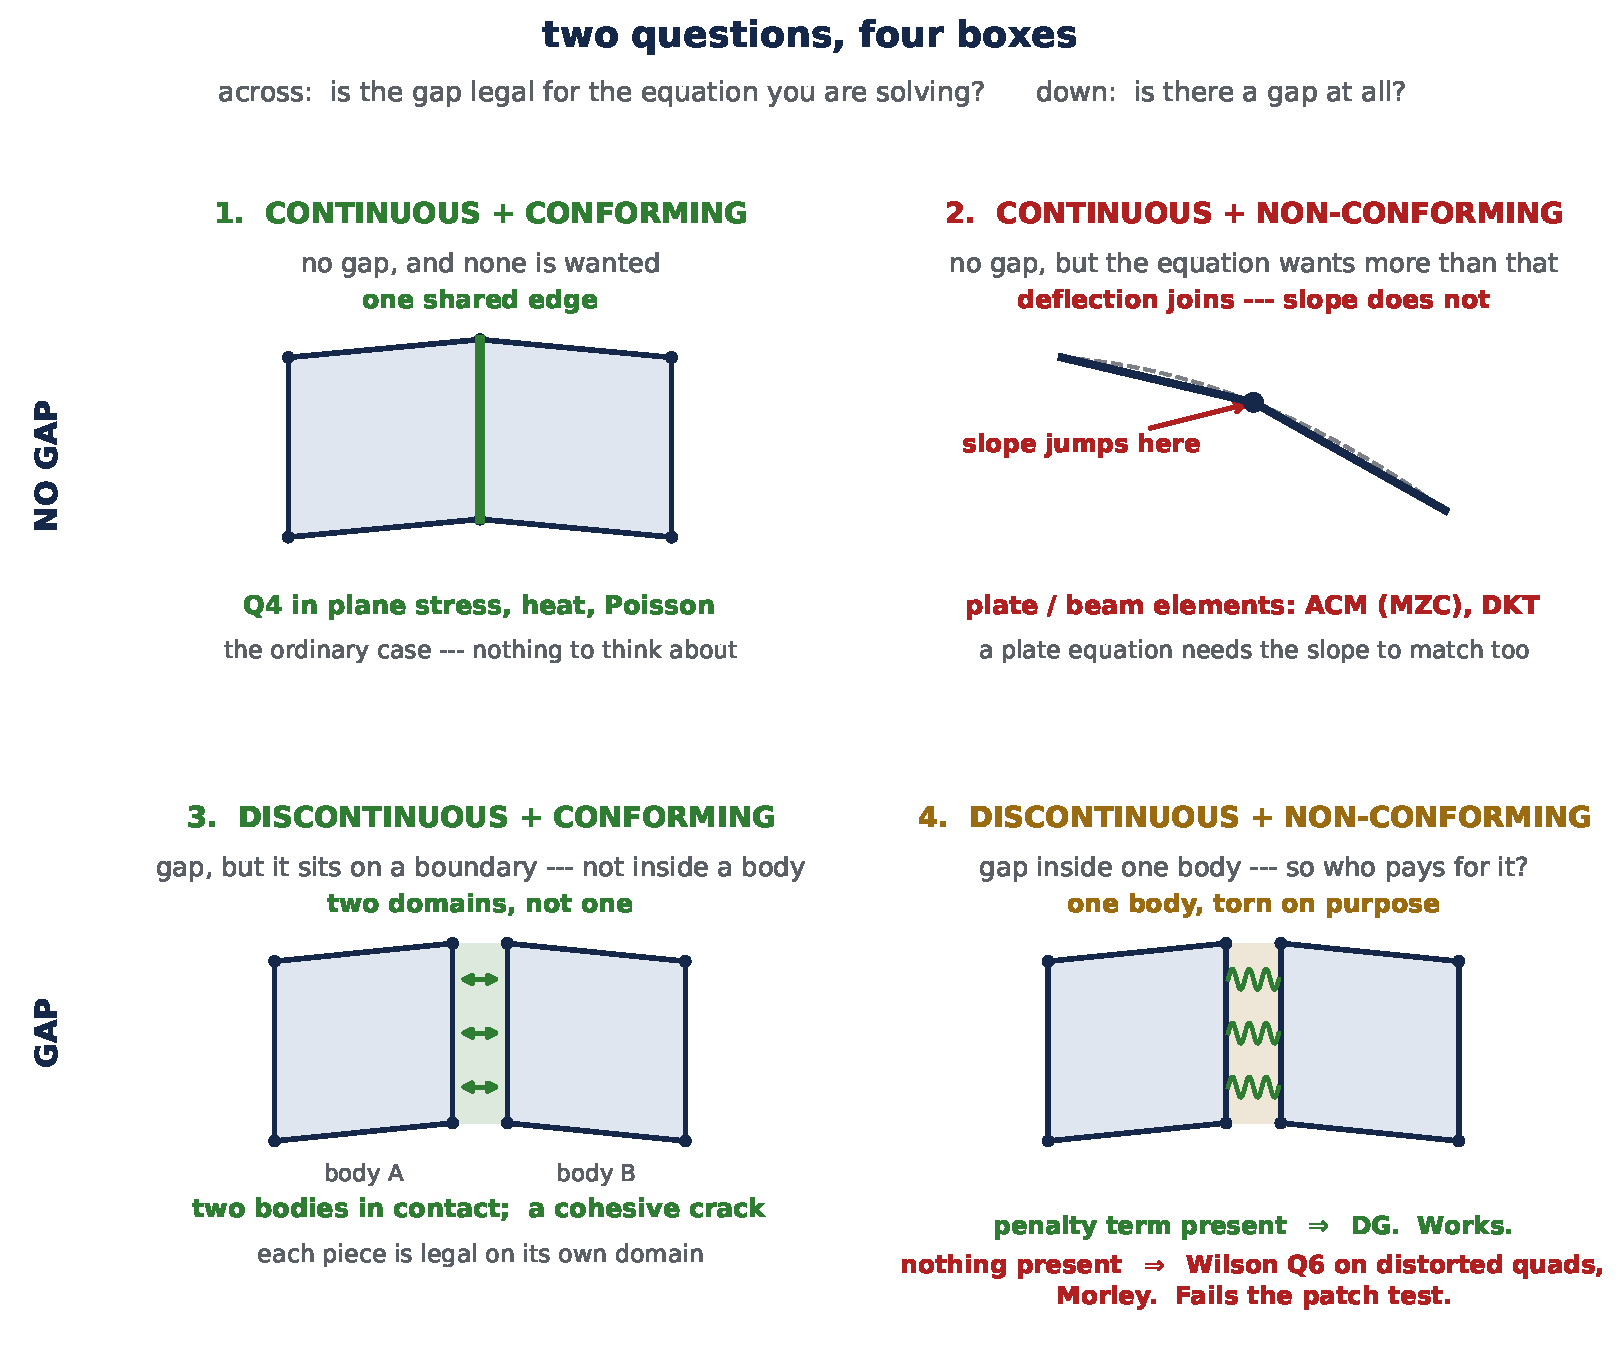
\includegraphics[width=0.93\linewidth]{q4_three_questions.pdf}
\captionof{figure}{The four combinations, all drawn on the same two elements.
\textbf{1:} the ordinary case. \textbf{2:} no gap at all, yet still
non-conforming --- a plate equation asks for the \emph{slope} to match too, and
it does not. \textbf{3:} a real gap that is still legal, because it lies on a
boundary between two bodies rather than inside one. \textbf{4:} a gap inside
one body, where everything depends on whether the weak form has a term that
pays for it --- a penalty (DG, which works) or nothing at all (Wilson Q6 on
distorted quads, Morley, which fails the patch test).}
\label{fig:fourboxes}
\end{center}

\medskip
\noindent\fbox{\parbox{0.955\linewidth}{\small
\textbf{The definition is one line: $V_{h}\subset V$.} The space you actually
compute in has to be a genuine \emph{subspace} of the space the weak form
lives in. Note what that is not: it is not a property of an element on its
own. A single Q4 is neither conforming nor non-conforming. It is a statement
about how two elements \emph{join}.

\medskip
What it costs depends on the order of the PDE, because that is what fixes $V$:

\medskip
\centering
\renewcommand{\arraystretch}{1.35}
\begin{tabular}{@{}llll@{}}
\toprule
the problem & $V$ & conforming means & so the element is\\
\midrule
bar, heat, plane stress, & $H^{1}$ & $C^{0}$: $v$ continuous, & Q4, T3 ---\\
Poisson & & $\grad v$ \emph{may} jump & cheap\\
\addlinespace[3pt]
beam, plate, biharmonic & $H^{2}$ & $C^{1}$: $v$ \emph{and} $\grad v$
                                    continuous, & Hermite in 1D;\\
 & & $v''$ \emph{may} jump & Argyris, $21$ DOF, in 2D\\
\bottomrule
\end{tabular}

\medskip
\raggedright
Your cantilever is the second row. CG(3) Hermite carries the value \emph{and}
the slope as nodal unknowns, and both are shared by the two elements meeting
at a node --- so $u_{h}$ is $C^{1}$ and $V_{h}\subset H^{2}$. The price of the
same thing in 2D is Lecture~13's Argyris element: $21$ degrees of freedom on
one triangle, second derivatives carried as nodal unknowns.

\medskip
\textbf{Why the lecture cares.} If $V_{h}\not\subset V$ then $B(v_{h},v_{h})$
is not merely wrong, it is \emph{undefined}: a jump in $v$ puts a $\delta$ in
$\grad v$ and $\iint\|\grad v\|^{2}=\infty$. Lax--Milgram, Galerkin
orthogonality and C\'ea are all stated on $V_{h}\subset V$. Lose it and every
error estimate in Lecture~13 goes with it --- which is why the lecture spends
$21$ degrees of freedom to keep it.

\medskip
\textbf{And that is what the two zeros were.} On $s=-1$,
$(N_{1},N_{2},N_{3},N_{4})=\bigl(\tfrac{1-r}{2},\tfrac{1+r}{2},0,0\bigr)$. The
zeros say the trace on that edge cannot possibly depend on nodes $3$ and $4$
--- the two the neighbour does \emph{not} share. So both elements build the
same function from the same two numbers, $u_{h}$ is continuous, $V_{h}\subset
H^{1}$. \S2 proved it from the polynomial; the table proves it from the
basis.}}

\medskip
\noindent\fbox{\parbox{0.955\linewidth}{\small
\raggedright
\textbf{So what is \emph{non}-conforming FEA?} Giving up $V_{h}\subset V$ on
purpose, and replacing the guarantee with a weaker one that still works.

\outside{non-conforming elements and the patch test}{%
\textbf{The one you have met.} \emph{Incompatible modes} --- Wilson's Q6 /
QM6. Add two internal bubbles to the Q4 field,
\[
  u=\sum_{a}N_{a}u_{a}+a_{1}(1-r^{2})+a_{2}(1-s^{2}).
\]
On the edge $s=-1$ the second bubble dies but the first does not, so the edge
displacement goes \emph{quadratic} in $r$ while the neighbour's $a_{1}$ is
independent of yours --- a gap opens along the shared edge. Deliberately
non-conforming, and done because it cures Q4's shear locking in bending: the
$xy$ term alone cannot bend without generating parasitic shear.

\medskip
\textbf{The other big family: plates.} $C^{1}$ in 2D costs $21$ DOF, so most
production plate elements (Morley, DKT, ACM) decline to pay and are
non-conforming.

\medskip
\textbf{What replaces the guarantee.} In engineering, the \textbf{patch
test}: load a patch of elements with boundary data consistent with a constant
strain state, and demand the element reproduce it \emph{exactly}. In the
mathematics, \textbf{Strang's second lemma}: the error bound picks up an extra
\emph{consistency} term measuring how far $B_{h}(u,v_{h})-L(v_{h})$ is from
zero. They are the same condition. Pass it and you still converge; fail it and
the element can converge confidently to the wrong answer --- which several
early plate elements did.}

\medskip
\textbf{The three different ``conforming''s.} This is where the confusion
usually comes from --- the word is doing three unrelated jobs:

\medskip
\centering
\renewcommand{\arraystretch}{1.35}
\begin{tabular}{@{}lll@{}}
\toprule
the phrase & what it is about & the condition\\
\midrule
\textbf{conforming element} & the approximation space & $V_{h}\subset V$\\
(engineering: ``compatible'') & & \\
\addlinespace[3pt]
\textbf{conforming mesh} & how elements are laid out & faces meet whole-face\\
 & & to whole-face; no hanging nodes\\
\addlinespace[3pt]
\textbf{compatibility} & a strain field & Saint-Venant: $\bm{\varepsilon}$ comes from\\
(solid mechanics) & & a single-valued $\bm{u}$\\
\bottomrule
\end{tabular}

\medskip
\raggedright
Only the first is what the lecture means. The second is a \emph{meshing}
property --- you can mesh a perfectly conforming Q4 non-conformingly, with
hanging nodes, and lose $V_{h}\subset V$ that way instead. The third has
nothing to do with either.}}

\bigskip
\noindent
\textbf{When is a jump an error, and when is it the answer?}
{\color{red!65!black}\textbf{[not from lecture]}} Three cases, all three
actually solved to draw the figure --- nothing in it is sketched by hand.

\begin{center}
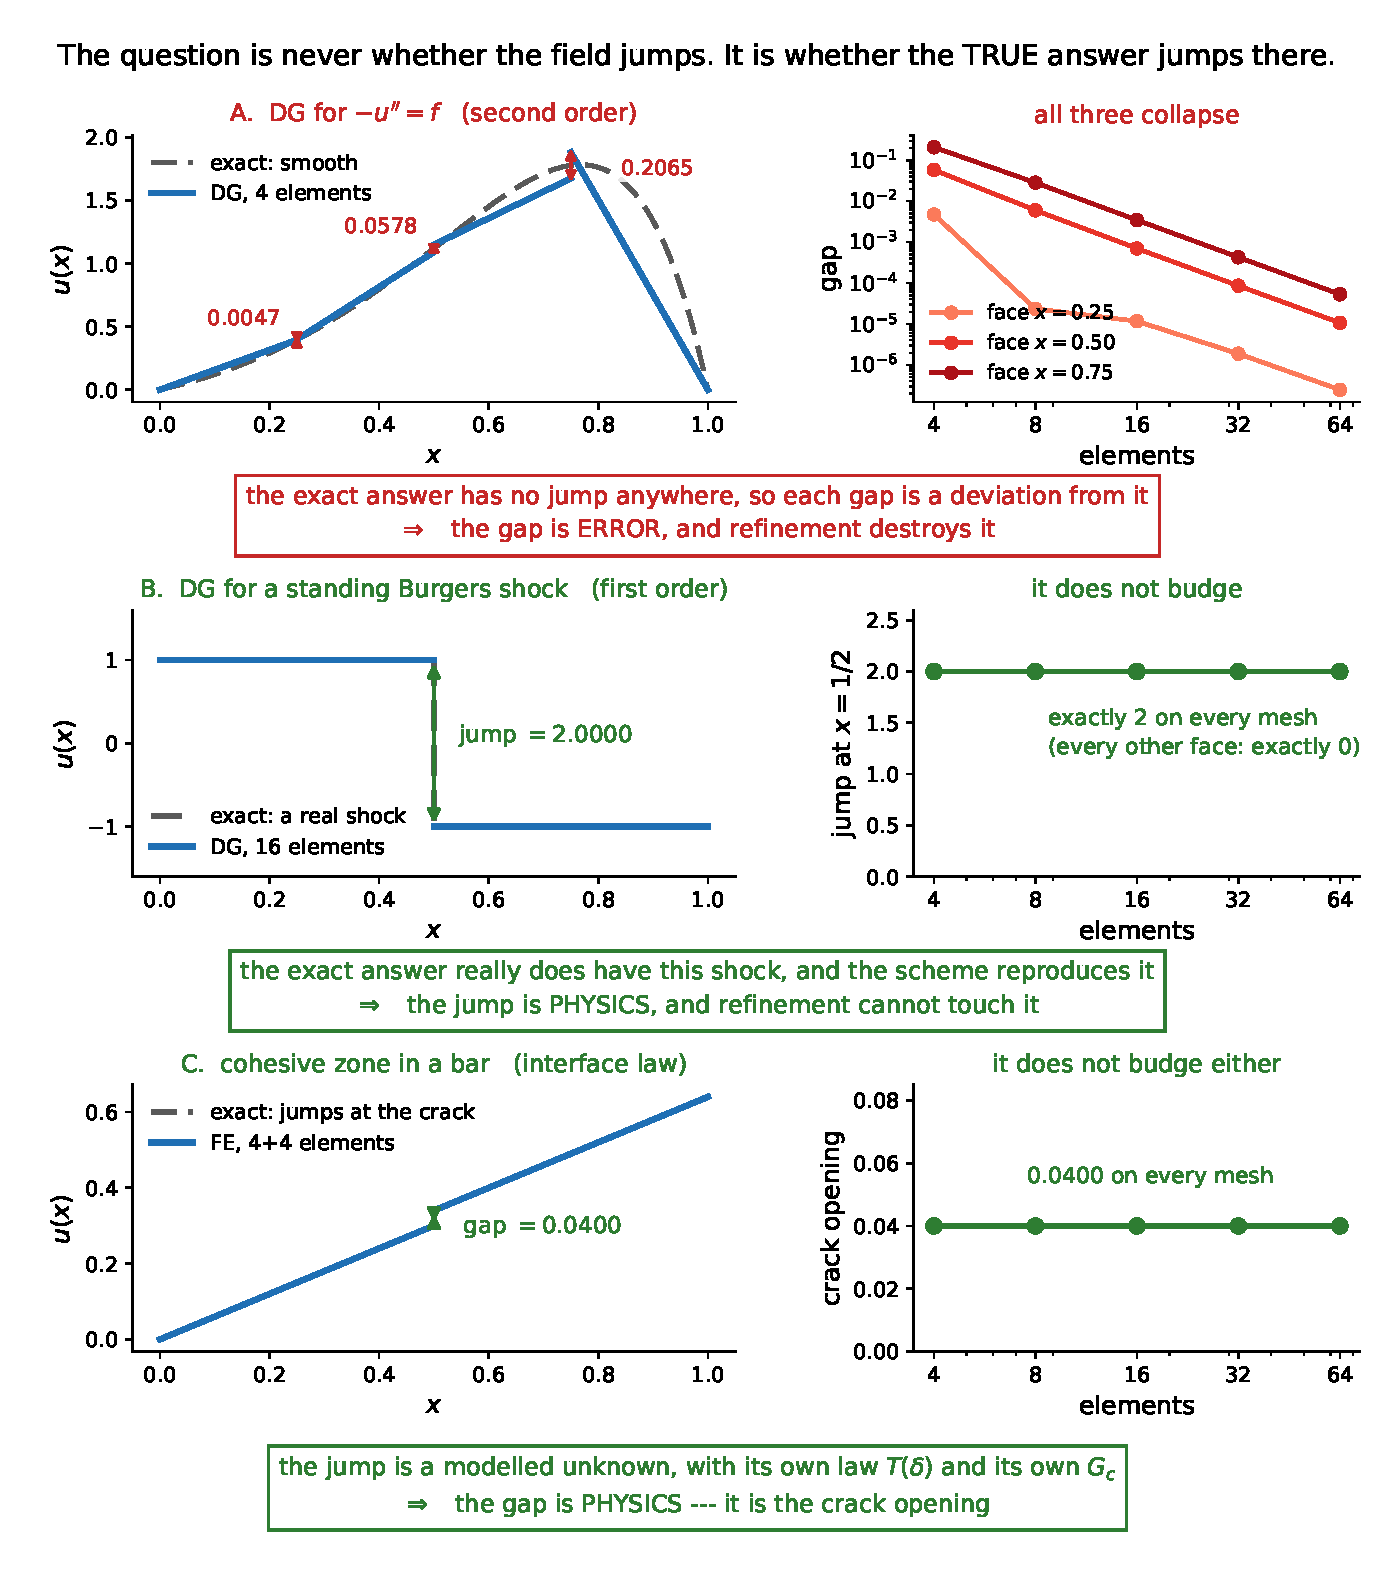
\includegraphics[width=\linewidth]{q4_three_jumps.pdf}
\captionof{figure}{Three fields that all jump at an interface, each one
actually solved rather than sketched. \textbf{A:} interior-penalty DG on
$-u''=f$, where the exact solution is smooth, so every jump is pure
discretisation error and vanishes under refinement. \textbf{B:} DG on a
stationary shock, where the exact solution really is discontinuous and the
jump is the answer, not an error. \textbf{C:} a cohesive zone, where the jump
is the crack opening and is set by the traction--separation law, not by the
mesh. Same picture, three different meanings --- which is the whole point.}
\label{fig:threejumps}
\end{center}

\medskip
\noindent
In all three the field jumps, by construction. What separates them is
\textbf{whether the \emph{true} answer jumps there}:

\begin{center}\small
\renewcommand{\arraystretch}{1.3}
\begin{tabular}{@{}llll@{}}
\toprule
 & A: DG, $-u''=f$ & B: DG, a shock & C: cohesive zone\\
\midrule
nodes doubled & every face & every face & the crack path only\\
true answer jumps there? & no \xmark & yes \cmark & yes \cmark\\
so the gap is & error & physics & physics\\
refine the mesh & $\to0$ & stays $2.0000$ & stays $0.0400$\\
\bottomrule
\end{tabular}
\end{center}

\medskip
\noindent
\textbf{That is a test you can actually run.} Refine and watch the gap. If it
shrinks, it was discretisation error. If it settles on a number you could
measure in a lab, it was physics.

\medskip
\noindent
\textbf{And now the part that trips everyone up: conformity is a
\emph{different} question, and it does not line up with that table.} Measured
against an $H^{1}$-type space --- the one a second-order equation forces on
you --- \textbf{A and B are \emph{both} non-conforming}: DG breaks the space
either way, and column~B's upwind flux is a jump penalty too, its size merely
fixed by the physics, $\tfrac12|\beta\!\cdot\!n|$, instead of tuned. Column
\textbf{C} is conforming, because the continuum model \emph{itself} admits a
jump on the crack plane.

\medskip
\noindent
But B's label is not even stable, and that is the real lesson. Write the
first-order problem in \emph{flux} form --- every derivative moved onto the
test function --- and the trial space needs no derivative at all, broken
polynomials sit inside it, and the same method is \emph{conforming}. Write it
in graph form, $\{v:\beta\!\cdot\!\nabla v\in L^{2}\}$, and a jump across a
face puts a $\delta$ into $\beta\!\cdot\!\nabla v$, so it is
\emph{non-conforming}. Same method, same mesh, same answer --- two labels,
because two different $V$'s were written down. So: \textbf{never ask ``is DG
conforming?''\ Ask ``non-conforming with respect to \emph{what}?''} There are
only three possible answers, and they live in different sentences:

\begin{center}\small
\renewcommand{\arraystretch}{1.3}
\begin{tabular}{@{}lll@{}}
\toprule
sense & the claim is about & carries a theorem?\\
\midrule
the \textbf{space} & $V_{h}\not\subset V$, with $V$ fixed by \emph{your} weak form
                   & yes --- it decides which error analysis applies\\
the \textbf{mesh}  & hanging nodes, non-matching faces & no\\
\textbf{neither}   & local slang for ``not the standard CG element'' & no\\
\bottomrule
\end{tabular}
\end{center}

\noindent
Only the first carries any content, and even it is relative. The method's
behaviour never changes when the label does --- only the yardstick does.
\textbf{The gap-under-refinement test is worth more than any of the three
labels}, because it is a property of your problem rather than of somebody's
vocabulary.

\medskip
\noindent
Two more traps in the vocabulary while we are here.
\begin{itemize}[leftmargin=1.4em, topsep=3pt, itemsep=3pt]
\item \textbf{Non-conforming does not mean inconsistent.} Interior-penalty DG
      is \emph{consistent}: the exact solution satisfies the discrete
      equations exactly, so the Strang consistency term is identically zero
      and Galerkin orthogonality still holds in $B_{h}$. Wilson's Q6 and
      Morley are non-conforming \emph{and} inconsistent --- which is exactly
      why \emph{they} need a patch test and DG does not. The patch test
      belongs to the classical non-conforming elements, not to DG.
\item \textbf{``Discrete'' is not a third kind of continuity.} Discrete means
      finite-dimensional --- you replaced a PDE by $N$ unknowns. \emph{Every}
      finite element method is discrete, CG and DG alike. Continuous versus
      discontinuous is a separate axis: whether the approximation is allowed
      to jump across a face.
\end{itemize}

\medskip
\noindent
Which sense a book means depends on which building it was written in.
\textbf{Ern--Guermond} and \textbf{Di~Pietro--Ern} --- this course's dialect ---
always use the space sense and always \emph{name} the space: ``the approximation
setting in dG methods is nonconforming since functions in $V_{h}$ can jump
across the mesh interfaces, whereas membership in $V:=H^{1}_{0}$ requires
continuity''. They are not saying DG is non-conforming full stop; they are
saying it is non-conforming \emph{against $H^{1}_{0}$}, which is the space
their chapter is about. \textbf{Computational mechanics} (Zienkiewicz--Taylor
and the whole conforming/compatible versus incompatible tradition) uses the
blanket sense and settles it with the patch test. And in \textbf{CFD and the
hyperbolic DG world --- the one your MOOSE work sits in} --- ``non-conforming''
most often means the \emph{mesh}: hanging nodes and non-matching faces, nothing
to do with function spaces at all.

\medskip
\noindent\fbox{\parbox{0.955\linewidth}{\small
\raggedright
\textbf{The intuition: $\det\bm{J}$ is a \emph{local} stretch, not a global
one.} Picture the reference square as a rubber sheet ruled with a uniform
grid. The map pulls it onto $D$, and because $D$ is not a rectangle the sheet
is stretched \emph{unevenly}: a small patch of reference area becomes a larger
physical patch in some parts of the element and a smaller one in others.
$\det\bm{J}$ at a point is exactly that local magnification. Four Gauss points
sit in four different places, so they see four different magnifications.

\medskip
You can read it off $D$'s shape. Compare how \emph{open} its corners are ---
the triangle cut off at each node has area
\[
  \text{node }1:\ \tfrac{15}{2},\qquad
  \text{node }2:\ 6,\qquad
  \text{node }3:\ \tfrac{13}{2},\qquad
  \text{node }4:\ 8 .
\]
Node~$4$ at $(1,5)$ is the widest corner and node~$2$ at $(3,0)$ the tightest,
so the map stretches most towards $(r,s)=(-1,1)$ and least towards $(1,-1)$.
The Gauss points follow exactly that: $q4$ (nearest the open corner) carries
the \emph{largest} value, $3.789$, and $q2$ (nearest the tight one) the
\emph{smallest}, $3.211$. ``Nearest'' is not a coincidence: the $2\times2$
points are ordered $(-g,-g),(g,-g),(g,g),(-g,g)$, the same cycle as the nodes,
so $q_{a}$ always sits in node $a$'s quadrant --- before the map and after it.

\medskip
\textbf{The check that ties it together.} Each Gauss point carries
$w_{q}\det\bm{J}_{q}$ of physical area --- its own share of the element. Add
them up:
\[
  \sum_{q=1}^{4}w_{q}\det\bm{J}_{q}
  =3.644338+3.211325+3.355662+3.788675=14.000000,
\]
exactly the area of $D$. So the four numbers are not four competing answers;
they are four pieces of one element, and the quadrature weights every
integrand value by how much physical area its point stands for. (This sum is
exact because $\det\bm{J}$ is \emph{linear} in $r,s$ --- it is the
\emph{ratio} in \eqref{eq:rational} that the rule cannot handle.)}}

\medskip
\noindent\fbox{\parbox{0.955\linewidth}{\small
\textbf{Two questions the picture has to answer --- (a) the node pairing.}

\medskip
\textbf{(a) Must $(x,y)=(0,0)$ sit at $(r,s)=(-1,-1)$?}
\textbf{No --- that is this element's node numbering, nothing more.}
Whichever corner you choose to call node~$1$ goes to $(-1,-1)$; node~$2$ to
$(1,-1)$, node~$3$ to $(1,1)$, node~$4$ to $(-1,1)$.


\medskip
The table in the figure box above is the whole of it: at a parent corner three
of the four $N_{a}$ vanish and the fourth is $1$, so $\sum_{a}N_{a}x_{a}$ hands
back \emph{whichever} nodal coordinate you happened to put in that slot.
\textbf{Nothing in that calculation knows which physical corner is which} --- it only reads the list $(x_{a},y_{a})$ you supplied.
Start $D$'s corner list at a different corner, still going counter-clockwise,
and you get the \emph{same element}, relabelled:

\medskip
\centering
\renewcommand{\arraystretch}{1.3}
\begin{tabular}{@{}lll@{}}
\toprule
list starts at & $\det\bm{J}(r,s)$ & at nodes $1,2,3,4$\\
\midrule
$(0,0)$ & $\tfrac72-\tfrac{3r}{8}+\tfrac{s}{8}$
        & $\tfrac{15}{4},\ 3,\ \tfrac{13}{4},\ 4$\\
$(3,0)$ & $\tfrac72+\tfrac{r}{8}+\tfrac{3s}{8}$
        & $3,\ \tfrac{13}{4},\ 4,\ \tfrac{15}{4}$\\
$(4,4)$ & $\tfrac72+\tfrac{3r}{8}-\tfrac{s}{8}$
        & $\tfrac{13}{4},\ 4,\ \tfrac{15}{4},\ 3$\\
$(1,5)$ & $\tfrac72-\tfrac{r}{8}-\tfrac{3s}{8}$
        & $4,\ \tfrac{15}{4},\ 3,\ \tfrac{13}{4}$\\
\bottomrule
\end{tabular}

\medskip
\raggedright
The same four numbers every time, just rotated around; the area is $14$ in all
four. What is \emph{not} free is the direction you go round. List $D$'s corners
\emph{clockwise} and $\det\bm{J}=\tfrac{3r}{8}+\tfrac{s}{8}-\tfrac72$, giving
$-4,-\tfrac{13}{4},-3,-\tfrac{15}{4}$ \xmark\ --- all four negative. The two
kinds of swap are not alike, and it is worth knowing which is which:
\emph{opposite} nodes ($1\!\leftrightarrow\!3$ or $2\!\leftrightarrow\!4$)
merely reverses the traversal, so you land back on the clockwise case
($-\tfrac{13}{4},-3,-\tfrac{15}{4},-4$) and the quadrilateral stays simple ---
which is exactly why that swap is the \emph{cure} for a clockwise list.
\emph{Adjacent} nodes ($2\!\leftrightarrow\!3$, say) is the damaging one: it
gives $4,-3,-\tfrac{13}{4},\tfrac{15}{4}$ \xmark, mixed signs, the bow-tie.
So \textbf{which} corner you start at is a free choice;
\textbf{the cyclic order is not} --- and it is not a per-element whim either,
since the element across a shared edge must list that edge's two nodes the same
way or the two images of the edge will not coincide.}}

\medskip
\noindent\fbox{\parbox{0.955\linewidth}{\small
\textbf{(b) Why does the grid run parallel to $D$'s edges instead of staying
square?}
\textbf{Because the edges \emph{are} grid lines.} They are not a separate
object drawn on top of the grid --- they are its outermost members:
\[
  r=-1\ \text{is edge }1\!-\!4,\quad
  r=+1\ \text{is edge }2\!-\!3,\quad
  s=-1\ \text{is edge }1\!-\!2,\quad
  s=+1\ \text{is edge }4\!-\!3 .
\]
Every line $r=c$ runs from edge $1\!-\!2$ to edge $4\!-\!3$ and interpolates
between edges $1\!-\!4$ and $2\!-\!3$ on the way, so of course it looks like
them. It does \emph{not} stay parallel to the $r$ and $s$ axes, because the map
is not the identity --- it rotates, stretches and shears. Only for a rectangle
with edges along $x$ and $y$ would the image grid come out axis-parallel.

\medskip
\textbf{And the lines are not parallel to \emph{one another} either.} Each
image is still perfectly \emph{straight} --- along $r=c$ both $x$ and $y$ are
affine in $s$ --- but the family fans:
\begin{center}\small
\renewcommand{\arraystretch}{1.2}
\begin{tabular}{@{}lccccc@{}}
\toprule
line & $-1$ & $-\tfrac12$ & $0$ & $\tfrac12$ & $+1$\\
\midrule
slope of $r=\text{const}$ & $5$ & $\tfrac{19}{4}$ & $\tfrac92$ & $\tfrac{17}{4}$ & $4$\\
slope of $s=\text{const}$ & $0$ & $-\tfrac1{12}$ & $-\tfrac16$ & $-\tfrac14$ & $-\tfrac13$\\
\bottomrule
\end{tabular}
\end{center}
\noindent
The endpoints of each row are just the slopes of the two opposite edges of $D$
--- $5$ and $4$ for edges $1\!-\!4$ and $2\!-\!3$, $0$ and $-\tfrac13$ for
edges $1\!-\!2$ and $4\!-\!3$ --- and the interior lines rotate smoothly from
one to the other. \textbf{The fan is the distortion.} Make $D$ a
parallelogram and opposite edges become parallel, each row collapses to a
single slope, the image grid becomes a true parallelogram grid --- and that is
the \emph{same} condition that makes $\det\bm{J}$ constant.}}

\medskip
\noindent\fbox{\parbox{0.955\linewidth}{\small
\textbf{Is $\det\bm{J}$ the same at the four parent corners?} It depends on
the element. Put all of them through it, together with a fifth, $E$, a
$10\times10$ square with corners $(0,0),(-10,0),(-10,-10),(0,-10)$:

\medskip
\centering
\renewcommand{\arraystretch}{1.3}
\begin{tabular}{@{}llll@{}}
\toprule
element & shape & $\det\bm{J}(r,s)$ & at nodes $1,2,3,4$\\
\midrule
$A$ & square $1\times1$     & $\tfrac14$ & $\tfrac14,\ \tfrac14,\ \tfrac14,\ \tfrac14$\\
$B$ & rectangle $2\times2$  & $1$        & $1,\ 1,\ 1,\ 1$\\
$C$ & rectangle $3\times1$  & $\tfrac34$ & $\tfrac34,\ \tfrac34,\ \tfrac34,\ \tfrac34$\\
$E$ & square $10\times10$   & $25$       & $25,\ 25,\ 25,\ 25$\\
$D$ & general convex quad   & $\tfrac72-\tfrac{3r}{8}+\tfrac{s}{8}$
                            & $\tfrac{15}{4},\ 3,\ \tfrac{13}{4},\ 4$\\
\bottomrule
\end{tabular}

\medskip
\raggedright
$A$, $B$, $C$, $E$ all give four \emph{equal} values; only $D$ does not. The
case where they are equal has a name.

\medskip
\textbf{(i) Constant $\det\bm{J}$ $\iff$ the element is a parallelogram.}
The $rs$ coefficient of the map is
\[
  x(r,s)\ \text{has}\ rs\text{-coefficient}\ \tfrac14(x_{1}-x_{2}+x_{3}-x_{4}),
  \qquad
  y(r,s)\ \text{has}\ \tfrac14(y_{1}-y_{2}+y_{3}-y_{4}),
\]
and both vanish exactly when $x_{3}=x_{2}+x_{4}-x_{1}$, $y_{3}=y_{2}+y_{4}-y_{1}$
--- the definition of a parallelogram. With no $rs$ term the map is affine,
$\bm{J}$ is a constant matrix, and every corner gives the same $\det\bm{J}$.
A rectangle is the special case. For $D$:
$y_{1}-y_{2}+y_{3}-y_{4}=0-0+4-5=-1\neq0$ \xmark\ --- not a
parallelogram, so $\det\bm{J}$ must vary. (Its $x$ counterpart is
$0-3+4-1=0$, which is why $x(r,s)$ in \eqref{eq:fwdD} has no $rs$ term while
$y(r,s)$ does.)

\medskip
\textbf{(ii) $\det\bm{J}$ is always \emph{affine} in $(r,s)$ --- never
bilinear.} Working it out for a quad with arbitrary corners, the $rs$ term of
$\det\bm{J}$ \emph{cancels identically}:
\[
  \det\bm{J}=\alpha+\beta r+\gamma s \qquad\text{(no $rs$ term, for any Q4).}
\]
That has a practical consequence: an affine function on a square attains its
maximum and minimum \textbf{at the corners}. So testing $\det\bm{J}>0$ at the
four corners certifies it is positive \emph{everywhere} in the element --- no
interior check needed. This is exactly why a mesher's element-quality routine
reports \emph{corner} Jacobians.

\medskip
\textbf{(iii) The four corner values average to the centre value.} Again
because $\det\bm{J}$ is affine,
\[
  \tfrac14\bigl(3.75+3+3.25+4\bigr)=3.5=\det\bm{J}\bigl|_{(0,0)},
  \qquad
  3.5\times\underbrace{4}_{\text{reference area}}=14=\text{area of }D .
\]
So the corner Jacobians are not four unrelated numbers: their mean is the
element's average magnification, and that times the reference area is the area.

\medskip
\textbf{(iv) Two things element $E$ makes visible.} First, \emph{scale}:
$E$ has $100\times$ the area of $A$ and exactly $100\times$ its
$\det\bm{J}$ ($25$ against $\tfrac14$). $\det\bm{J}$ is an area magnification,
so it grows with the square of the element size --- halving a mesh divides
every $\det\bm{J}$ by four.

\medskip
Second, a trap. $E$'s map is
\[
  x(r,s)=-5r-5,\qquad y(r,s)=-5s-5,
  \qquad\text{so}\qquad
  \bm{J}=\begin{bmatrix}-5&0\\0&-5\end{bmatrix},
  \qquad \det\bm{J}=(-5)(-5)-0=+25 .
\]
\textbf{Both} entries of $\bm{J}$ are negative --- $x$ \emph{decreases} as $r$
increases, and likewise $y$ with $s$ --- yet $\det\bm{J}>0$ and the element is
perfectly valid. Flipping \emph{two} axes is a $180^{\circ}$ rotation, not a
reflection, so orientation is preserved. The lesson: \textbf{never read the
signs of the individual entries of $\bm{J}$; read $\det\bm{J}$.} Only an
\emph{odd} number of flips inverts an element.

\medskip
\textbf{Caveat.} All three statements are specific to the \emph{bilinear} Q4.
For a quadratic element (Q8/Q9) or a curved edge, $\det\bm{J}$ is no longer
affine, its extrema can sit in the interior, and checking only the corners is
\emph{not} sufficient.}}

\medskip
\noindent\fbox{\parbox{0.955\linewidth}{\small
\textbf{Four things about $\det\bm{J}$ worth carrying around.}

\medskip
\textbf{1. A corner Jacobian \emph{is} a triangle area.} At node $i$, let
$\bm{v}_{\text{next}}$ and $\bm{v}_{\text{prev}}$ be the two edge vectors
leaving it. Then
\[
  \det\bm{J}\big|_{\text{node }i}
  =\tfrac14\bigl(\bm{v}_{\text{next}}\times\bm{v}_{\text{prev}}\bigr)
  =\tfrac12\times\text{area of the triangle cut off at that corner}.
\]
For $D$ at node~$1$: neighbours $(3,0)$ and $(1,5)$, triangle area
$\tfrac{15}{2}$, half of it $\tfrac{15}{4}$ --- exactly the $\det\bm{J}$
tabulated above. \emph{Use:} you can estimate corner Jacobians \emph{by eye} ---
the more open the corner, the larger its Jacobian. A nearly-straight corner has
one near zero.

\medskip
\textbf{2. All four negative $\Rightarrow$ you numbered the nodes clockwise.}
Numbering $D$ backwards gives
$-\tfrac{15}{4},-4,-\tfrac{13}{4},-3$ --- same magnitudes, every
sign flipped. The element is fine; the \emph{connectivity} is reversed. Fix by
swapping two \emph{opposite} nodes ($1\!\leftrightarrow\!3$ or
$2\!\leftrightarrow\!4$), not by remeshing --- an \emph{adjacent} swap would
tangle it instead.

\medskip
\textbf{3. \emph{One} negative $\Rightarrow$ the element is genuinely tangled.}
A quad with a reflex (concave) corner at node~$3$ gives
$\;2,\ \tfrac14,\ -\tfrac32,\ \tfrac14\;$ --- and the negative one \emph{is}
the reflex corner. Mixed signs cannot be cured by renumbering. So the sign
pattern diagnoses the problem: \textbf{uniform sign $=$ orientation, mixed sign
$=$ geometry}.

\medskip
\textbf{4. $\det\bm{J}$ tells you nothing about skew.} Shear a unit
parallelogram by $k$ --- corners $(0,0),(1,0),(1{+}k,1),(k,1)$:
\begin{center}
\renewcommand{\arraystretch}{1.15}
\begin{tabular}{@{}lccccc@{}}
\toprule
$k$ & $0$ & $1$ & $3$ & $10$ & $50$\\
\midrule
$\det\bm{J}$     & $1/4$ & $1/4$ & $1/4$ & $1/4$ & $1/4$\\
area             & $1$ & $1$ & $1$ & $1$ & $1$\\
$\mathrm{cond}(\bm{J})$ & $1.0$ & $2.6$ & $10.9$ & $102$ & $2502$\\
\bottomrule
\end{tabular}
\end{center}
The determinant and the area never move, while the element becomes a worse and
worse sliver. \textbf{A healthy $\det\bm{J}$ does not mean a healthy element.}
That is why mesh-quality reports carry aspect ratio and skew \emph{separately}
from the Jacobian --- and why Lecture~13's regularity condition
$h_{j}/\rho_{j}\le\alpha$ is a statement about \emph{shape}, not about area.}}

\medskip
\noindent\fbox{\parbox{0.955\linewidth}{\small
\textbf{A worked case: element $F$, listed the wrong way round.} Take
$(0,0),\,(-2,2),\,(6,7),\,(4,-1)$ as nodes $1,2,3,4$ and run the whole
diagnosis above on it --- Figure~\ref{fig:elemF}.}}

\begin{center}
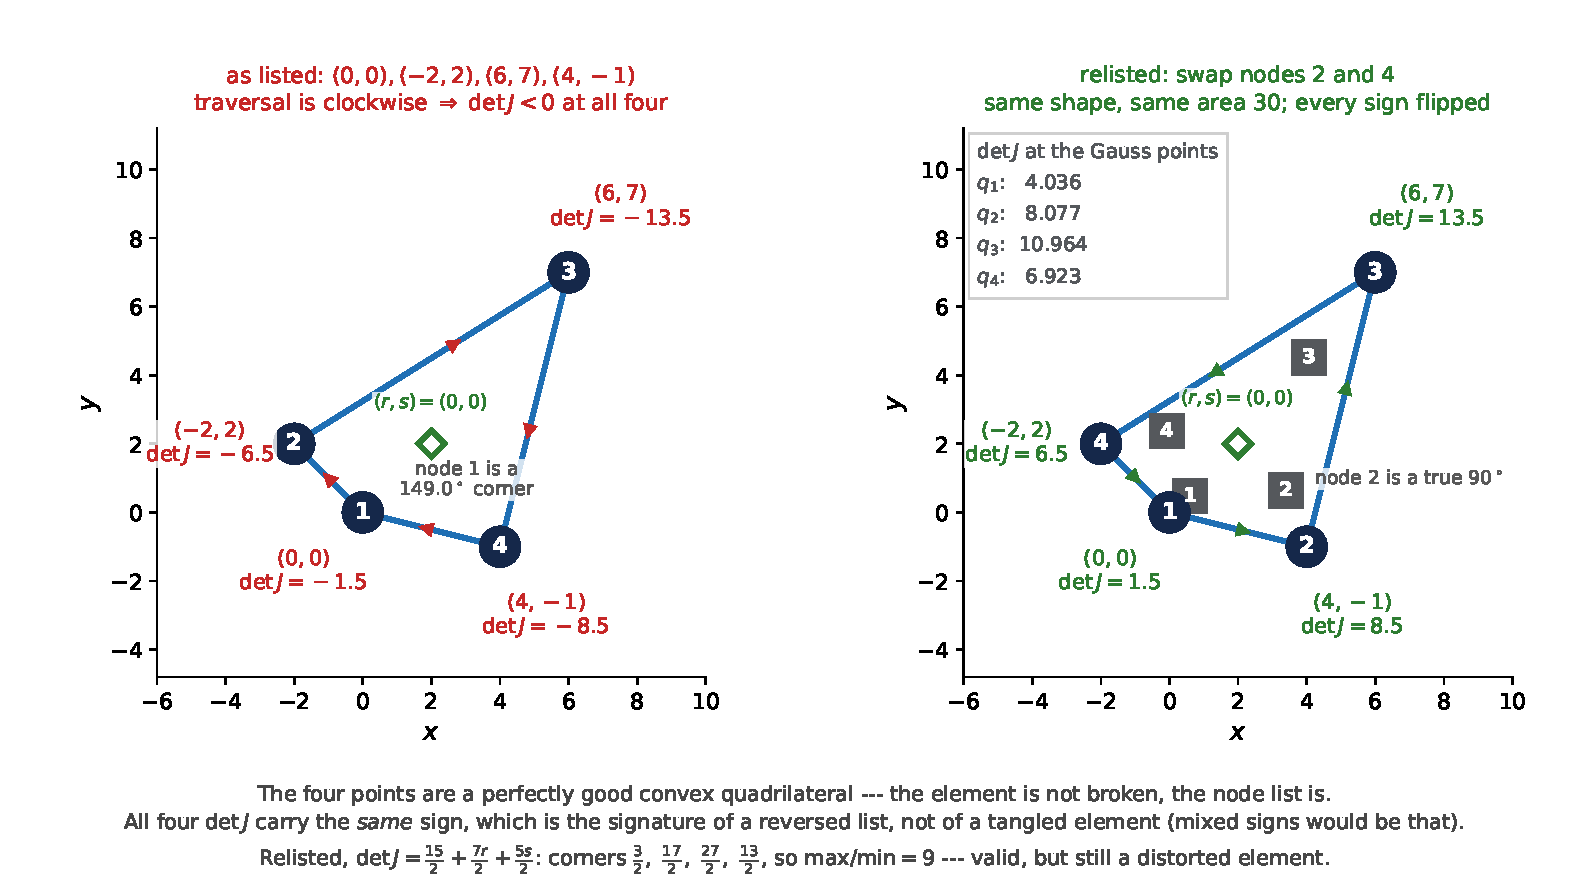
\includegraphics[width=\linewidth]{q4_elemF.pdf}
\captionof{figure}{Element $F$, the same four points listed two ways.
\textbf{Left:} as given, which traverses them clockwise --- $\det\bm{J}<0$ at
every Gauss point. \textbf{Right:} relisted counter-clockwise, same geometry,
$\det\bm{J}>0$ throughout. The shape was never the problem; the connectivity
order was.}
\label{fig:elemF}
\end{center}

\noindent\fbox{\parbox{0.955\linewidth}{\small
\textbf{The shape is fine.} No edge crosses another, and all four corner cross
products share a sign, so it is a simple \emph{convex} quadrilateral. Interior
angles $149.0^{\circ},77.0^{\circ},44.0^{\circ},90.0^{\circ}$ (sum
$360^{\circ}$ \cmark), area $30$.

\medskip
\textbf{The list is not.} As given,
\[
  x=2+3s+rs,\qquad
  y=2+\tfrac{5r}{2}+s+\tfrac{3rs}{2},\qquad
  \det\bm{J}=-\tfrac{15}{2}-\tfrac{5r}{2}-\tfrac{7s}{2},
\]
and at nodes $1,2,3,4$ that reads
$-\tfrac32,\ -\tfrac{13}{2},\ -\tfrac{27}{2},\ -\tfrac{17}{2}$ \xmark\ ---
four negatives. By point~2 a \emph{uniform} sign is an orientation report, not
a geometry report, and the shoelace sum confirms it: $2A=-60<0$, so the corners
were walked \textbf{clockwise}.

\medskip
\textbf{The repair is the one point~2 prescribes} --- swap two \emph{opposite}
nodes, here $2\leftrightarrow4$, giving $1{=}(0,0)$, $2{=}(4,-1)$, $3{=}(6,7)$,
$4{=}(-2,2)$:
\[
  x=2+3r+rs,\qquad
  y=2+r+\tfrac{5s}{2}+\tfrac{3rs}{2},\qquad
  \det\bm{J}=\tfrac{15}{2}+\tfrac{7r}{2}+\tfrac{5s}{2},
\]
with nodal values $\tfrac32,\ \tfrac{17}{2},\ \tfrac{27}{2},\ \tfrac{13}{2}$
\cmark --- the same four magnitudes, every sign flipped, exactly as point~2
says. The quadrature closes too:
$4.035898+8.077350+10.964102+6.922650=30$, the area.
\textbf{Nothing was remeshed.} One transposition in the connectivity array.

\medskip
\textbf{It is a valid element and a mediocre one, and these are separate
verdicts.} Its corner Jacobians span
$\max/\min=\tfrac{27/2}{3/2}=9$. Against the last box's scale --- $1$ for any
parallelogram --- that is still poor. Point~1 says where it comes from:
node~$1$ is a $149.0^{\circ}$ corner, so the triangle cut off there has area
only $3$ and half of it is $\det\bm{J}=\tfrac32$, while node~$3$'s triangle has
area $27$ and gives $\tfrac{27}{2}$. The element would pass every validity
check in this note and still integrate indifferently, because $\det\bm{J}$ in
the denominator of \eqref{eq:rational} swings by a factor of $9$ across it.

\medskip
(It is not a parallelogram, which is why $\det\bm{J}$ varies at all: the $rs$
coefficients are $\tfrac14(0-4+6+2)=1$ and $\tfrac14(0+1+7-2)=\tfrac32$,
neither zero, so test~(i) fails. Two things it \emph{does} have: the corner at
$(4,-1)$ is a true right angle, since $(4,-1)\cdot(2,8)=0$, and the edge
beyond it is exactly twice as long, $\sqrt{17}$ against $2\sqrt{17}$. Neither
helps --- $\det\bm{J}$ does not read angles, only areas.)}}

\medskip
\noindent\fbox{\parbox{0.955\linewidth}{\small
\textbf{Geometry as a variable --- what moves $\det\bm{J}$, and what does not.}
Each column below starts from the \emph{same} unit square, where
$\det\bm{J}=\tfrac14$ at all four nodes and at all four Gauss points, and then
changes exactly one number. The top row is the geometry; the bottom row is
$\det\bm{J}$ at the four corner nodes (coloured) and at the four Gauss points
(grey) as that number is swept.

\begin{center}
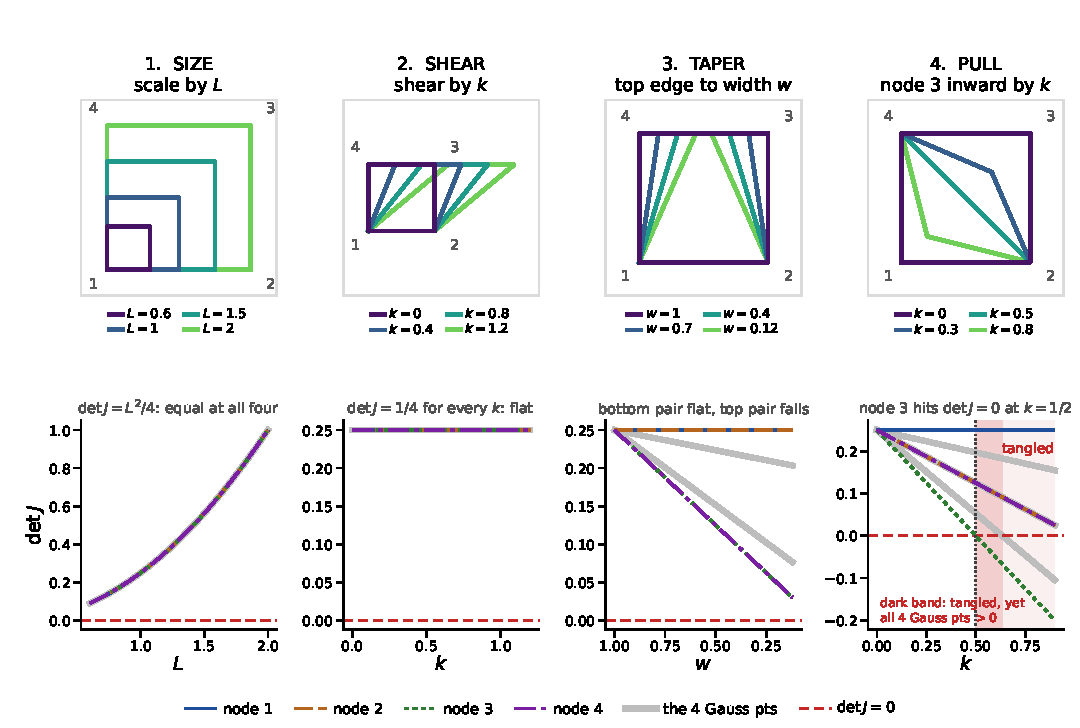
\includegraphics[width=\linewidth]{q4_geomstudy.pdf}
\captionof{figure}{Geometry as a variable: four one-parameter families, with
$\det\bm{J}$ computed from the nodal coordinates at the four corner nodes
(coloured) and the four Gauss points (grey) as the parameter is swept. SIZE
and SHEAR leave $\det\bm{J}$ constant --- both keep the element a
parallelogram. TAPER and PULL do not, and the spread between largest and
smallest is the measure of how far from a parallelogram the element has
drifted.}
\label{fig:geomstudy}
\end{center}

\medskip
\centering
\renewcommand{\arraystretch}{1.3}
\begin{tabular}{@{}llll@{}}
\toprule
family & $\det\bm{J}(r,s)$ & at nodes $1,2,3,4$ & $\max/\min$\\
\midrule
\addlinespace[2pt]
SIZE, $L$  & $L^{2}/4$ & all four $=L^{2}/4$ & $1$\\
\addlinespace[4pt]
SHEAR, $k$ & $1/4$ & all four $=1/4$ & $1$\\
\addlinespace[4pt]
TAPER, $w$ & $\bigl[(1+w)+(w-1)s\bigr]/8$
           & $\tfrac14,\ \tfrac14,\ \tfrac{w}{4},\ \tfrac{w}{4}$ & $1/w$\\
\addlinespace[4pt]
PULL, $k$  & $\bigl[2-2k-k(r+s)\bigr]/8$
           & $\tfrac14,\ \tfrac{1-k}{4},\ \tfrac{1-2k}{4},\ \tfrac{1-k}{4}$
           & $1/(1-2k)$\\
\addlinespace[2pt]
\bottomrule
\end{tabular}

\medskip
\raggedright
\textbf{1. SIZE --- $\det\bm{J}$ moves a lot; the element does not get worse.}
Scaling multiplies every $\det\bm{J}$ by $L^{2}$ and leaves all four equal. The
curve is a parabola, the four nodes sit on top of one another, and the Gauss
points sit on them too. Halving a mesh divides every $\det\bm{J}$ by four --- a
large change in the \emph{number} with no change at all in element
\emph{quality}.

\medskip
\textbf{2. SHEAR --- $\det\bm{J}$ does not move at all.} A dead-flat line at
$\tfrac14$ while the element slides into a sliver. This is point~4 of the
previous box drawn as a graph: the determinant is an area, and shearing
preserves area. \textbf{A flat $\det\bm{J}$ curve is not a certificate of a
good element.}}}

\medskip
\noindent\fbox{\parbox{0.955\linewidth}{\small
\textbf{Geometry as a variable, continued --- columns 3 and 4.}

\medskip
\textbf{3. TAPER --- the four values split into two pairs.} $\det\bm{J}$
depends on $s$ alone, so the bottom nodes $1,2$ hold $\tfrac14$ for every $w$
while the top nodes $3,4$ fall to $\tfrac w4$. This is the first case where
``the Jacobian of the element'' stops being a single number: at $w=0.12$ the
corner values are $\tfrac14,\tfrac14,0.03,0.03$ --- a factor of $8.3$ across
one element. Notice the grey curves lie strictly \emph{between} the coloured
ones: the Gauss points are interior, so they never attain the extreme values.

\medskip
\textbf{4. PULL --- a corner runs out.} Dragging node~$3$ in along the diagonal
makes $\det\bm{J}$ depend on both $r$ and $s$. Node~$1$ is untouched, nodes
$2$ and $4$ fall together, and node~$3$ falls twice as fast and reaches
\emph{zero} at $k=\tfrac12$. That is exactly where node~$3$ lands on the
straight line joining nodes $2$ and $4$: by point~1 of the previous box the
corner Jacobian \emph{is} half the area of the triangle cut off at that corner,
and at $k=\tfrac12$ that triangle has collapsed. Past $k=\tfrac12$ the sign
flips --- one negative corner, the mixed-sign pattern of a genuinely tangled
element.

\medskip
\textbf{The trap the fourth column was drawn for.} In the dark band,
$\tfrac12<k<\tfrac{3-\sqrt3}{2}\approx0.634$, the element is already tangled
--- node~$3$ has $\det\bm{J}<0$ --- and yet \textbf{all four $2\times2$ Gauss
points still return $\det\bm{J}>0$}. At $k=0.6$ the corners read
$0.25,\ 0.10,\ -0.05,\ 0.10$ while the Gauss points read
$0.187,\ 0.100,\ 0.013,\ 0.100$. A solver that tests only its quadrature points
accepts the element, assembles $\bm{k}^{e}$ from it, and reports nothing. The
reason is the affineness established two boxes back,
$\det\bm{J}=\alpha+\beta r+\gamma s$: its extremes sit at the \emph{corners},
while the Gauss points sit strictly inside at $\pm1/\sqrt3$ and can only ever
report values in between. \textbf{Test the corners, not the Gauss points.}

\medskip
\textbf{What to carry away.} $\det\bm{J}$ itself tells you size (column 1) and
validity (column 4). It tells you nothing about skew (column 2). The number
that tells you whether the mapping is \emph{distorted} is the \emph{spread} of
$\det\bm{J}$ across the element --- the last column of the table --- which is
$1$ for any parallelogram and grows without bound as a corner closes up. That
spread is the computational face of Lecture~13's shape-regularity condition.}}

\medskip
\noindent
A Gauss rule is constructed to integrate \emph{polynomials} exactly --- that is
the whole content of ``exact through degree $2n-1$''. The right-hand side of
\eqref{eq:rational} is not a polynomial: no finite-order Gauss rule integrates
it exactly, only ever approximately, and the approximation improves as points
are added. For $D$:
\begin{center}\small
\renewcommand{\arraystretch}{1.2}
\begin{tabular}{@{}lcccc@{}}
\toprule
rule & $2\times2$ & $3\times3$ & $6\times6$ & converged\\
\midrule
$k^{e}_{11}$ & $0.675085$ & $0.675272$ & $0.675272$ & $0.675272$\\
\bottomrule
\end{tabular}
\end{center}
\noindent
--- an error of about $0.03\%$ at $2\times2$, settled by about three points
per direction. In practice $2\times2$ is used for Q4 anyway and that small
quadrature error is accepted; the point here is only that ``exact'' is a claim
about rectangles, not about every element.

\medskip
Had we stayed in $x,y$ there would be no table to read from. The integration
limits would be the element's own edges, different for every element --- and
for a quad like $D$ not even expressible as constant limits --- so the
abscissae and weights would have to be rebuilt element by element. Mapping to
$[-1,1]^{2}$ is what turns integration into a fixed, four-line loop.

\medskip
\noindent
\textbf{The check that settles it.} Move the evaluation point to
$(r,s)=(1,1)$, which is node~$3$ itself. There
$N_{3}=1$ and $N_{1}=N_{2}=N_{4}=0$: node~$3$ takes the whole share. In
$A$, $B$ and $C$ this can be confirmed from the $x,y$ formula --- it gives $1$
at $(1,1)$, $(3,2)$ and $(5,4)$ respectively. \textbf{In $D$ there is no
formula to confirm it with, and yet the value is still exactly $1$} --- because
the nodal condition \eqref{eq:delta} is imposed in $(r,s)$, where every element
is the same square. We know the answer without being able to write the
function. That is the whole case for the reference square in one line.

\begin{center}\footnotesize
\renewcommand{\arraystretch}{1.35}
\setlength{\tabcolsep}{4.5pt}
\begin{tabular}{@{}llccccc@{}}
\toprule
 & & & \multicolumn{2}{c}{at the interior point $(r,s)=(0.5,0.5)$}
     & \multicolumn{2}{c}{at node $3$ itself, $(r,s)=(1,1)$}\\
\cmidrule(lr){4-5}\cmidrule(lr){6-7}
element & region & $N_{3}$ in $x,y$ & sits at $(x,y)=$ & node $3$'s share & sits at $(x,y)=$ & node $3$'s share\\
\midrule
$A$ & $[0,1]\times[0,1]$ & $x\,y$                  & $(0.75,\,0.75)$   & $0.5625$ & $(1,\,1)$          & $\bm{1}$\\
$B$ & $[1,3]\times[0,2]$ & $\tfrac14(x-1)\,y$      & $(2.50,\,1.50)$   & $0.5625$ & $(3,\,2)$          & $\bm{1}$\\
$C$ & $[2,5]\times[3,4]$ & $\tfrac13(x-2)(y-3)$    & $(4.25,\,3.75)$   & $0.5625$ & $(5,\,4)$          & $\bm{1}$\\
$D$ & a general quad     & \textcolor{red!60!black}{none}
                                                   & $(3,\,3.1875)$ & $0.5625$ & $(4,\,4)$   & $\bm{1}$\\
\midrule
\textbf{any} & --- & $\tfrac14(1+r)(1+s)$ & $(r,s)=(0.5,0.5)$ & $\bm{0.5625}$ & $(r,s)=(1,1)$ & $\bm{1}$\\
\bottomrule
\end{tabular}
\captionof{table}{The contribution of \emph{node $3$}, on four elements. Columns 4--5
read it at a general interior point, columns 6--7 at node $3$ itself. The
``sits at'' columns differ element by element and the $x,y$ formula differs
too --- but the two share columns do not. The last row is the only one a
program needs.}
\label{tab:why}
\end{center}

\noindent
\textbf{Row $D$ is the one that settles it.} in a arbitrary physical x-y co-ordinate mesh--  Given the quad the corners 
$(0,0)$, $(3,0)$, $(4,4)$, $(1,5)$, taken counter-clockwise from
local node~$1$. There is no formula in $x,y$ to evaluate --- the ``$N_{3}$ in
$x,y$ for local node 3'' column is empty. The physical point is found instead from the
\emph{isoparametric} map, defined next.

% ------------------------------------------------------------------
\subsubsection*{What ``isoparametric'' means}

\textbf{The name decodes directly.} \emph{Iso} $=$ same, \emph{parametric}
$=$ the shape functions. An element is \textbf{isoparametric} when the
\emph{same} shape functions are used for two different jobs:

\begin{center}\small
\renewcommand{\arraystretch}{1.5}
\begin{tabular}{@{}lll@{}}
\toprule
job & what is interpolated & written out\\
\midrule
interpolate the \textbf{unknown} & the nodal values $u_{a}$
  & $u_{h}\big|_{K}=\sum_{a=1}^{4}N_{a}(r,s)\,u_{a}$\\
interpolate the \textbf{geometry} & the nodal coordinates $(x_{a},y_{a})$
  & $x=\sum_{a=1}^{4}N_{a}(r,s)\,x_{a}$, \ \
    $y=\sum_{a=1}^{4}N_{a}(r,s)\,y_{a}$\\
\bottomrule
\end{tabular}
\end{center}

\noindent
Same $N_{a}$ in both rows. That --- and only that --- is the definition. It
also names the two alternatives, which is the distinction to have ready:

\begin{center}\small
\renewcommand{\arraystretch}{1.3}
\begin{tabular}{@{}l@{\hspace{1.2em}}l@{\hspace{1.2em}}p{6.1cm}@{}}
\toprule
 & geometry order & typical use\\
\midrule
\textbf{sub}parametric & \emph{lower} than the solution
  & straight-sided element carrying a quadratic solution\\
\textbf{iso}parametric & the \emph{same} as the solution
  & the standard choice; curved edges when the element is curved\\
\textbf{super}parametric & \emph{higher} than the solution & rare\\
\bottomrule
\end{tabular}
\end{center}

\medskip
\textbf{Why it is correct, not merely convenient.}  Take any linear field
$u=\alpha+\beta x+\gamma y$, sample it at the four corners, and interpolate:
\begin{equation}\label{eq:isoexact}
  u_{h}=\sum_{a}N_{a}u_{a}
      =\alpha\underbrace{\sum_{a}N_{a}}_{=\,1\ \text{by }\eqref{eq:pou}}
      +\beta\underbrace{\sum_{a}N_{a}x_{a}}_{=\,x\ \text{by the map}}
      +\gamma\underbrace{\sum_{a}N_{a}y_{a}}_{=\,y\ \text{by the map}}
      =\alpha+\beta x+\gamma y=u .
\end{equation}
The second and third underbraces are true \emph{because the map is built from
the same $N_{a}$} used in geometry interpolation. Choose a different set of N for
 geometry interpolation and than solution interpolation fails
. So the element passes the patch test by construction, on a distorted
quad as much as on a square regardless of the element shape.

\medskip
{\small\color{red!90}Checked on element $D$ with $u=2+3x-y$ (nodal values
$2,11,10,0$): at
$(r,s)=(0.5,0.5)$, $(-0.75,0.333)$, $(0,0)$ and $(0.9,-0.875)$ the
interpolated value equals the exact value of $u$ at the mapped point, to the
last digit of exact arithmetic.}

\medskip
\textbf{What the three $u$'s are.} \eqref{eq:isoexact} carries three symbols
that all look like ``$u$''. They are three different \emph{kinds} of object,
and the lectures use all three:

\begin{center}\small
\renewcommand{\arraystretch}{1.45}
\begin{tabular}{@{}l@{\hspace{1.0em}}p{4.4cm}@{\hspace{1.0em}}l@{\hspace{1.0em}}p{4.0cm}@{}}
\toprule
symbol & what kind of thing it is & lecture's symbol & on element $D$\\
\midrule
$u$ & a \textbf{function}, defined at every point of the domain
  & $u$
  & $u=2+3x-y$, the field you are testing with\\
$u_{a}$ & \textbf{numbers} --- one per node, four of them
  & $\xi_{j}$, the coefficients
  & $u_{1},\dots,u_{4}=2,\,11,\,10,\,0$\\
$u_{h}$ & a \textbf{function} again, but only one of those this mesh is able
          to build
  & $u_{h}\in V_{h}$
  & $u_{h}=\sum_{a}N_{a}u_{a}$\\
\bottomrule
\end{tabular}
\captionof{table}{The three objects \eqref{eq:isoexact} juggles. Two of them
are functions and one is a list of numbers --- which is why they cannot share
a symbol.}
\label{tab:threeus}
\end{center}

\textbf{Why one symbol will not do.} Because in general $u\neq u_{h}$, and the
gap between them \emph{is} the subject of the error analysis --- C\'ea's lemma
bounds $\norm{u-u_{h}}_{V}$, and you cannot write that quantity down if the
exact field and the computed field share a name. And $u_{a}$ is not a function
at all: it is the list of numbers the solver stores and solves for, which
$N_{a}$ turns back into a function. In the lecture's symbols the same three
are $u$, $\xi_{j}$, and $u_{h}=\sum_{j}\xi_{j}\varphi_{j}$ --- the only
translation needed is $N_{a}\leftrightarrow\varphi_{j}$ and
$u_{a}\leftrightarrow\xi_{j}$.

\medskip
\textbf{Reading \eqref{eq:isoexact} one step at a time.} The question it
answers is: \emph{hand the element a flat tilted plane --- does it give the
same plane back?}

\begin{enumerate}[leftmargin=1.6em,itemsep=0.3em,topsep=0.3em]
\item \textbf{The element only ever receives four numbers.} Visit each node,
  read its coordinates, evaluate the plane there:
  $u_{a}=\alpha+\beta x_{a}+\gamma y_{a}$. On element $D$ with $u=2+3x-y$
  those are $2,11,10,0$. The formula itself is then thrown away --- the
  element never sees it.

\item \textbf{Stand at an interior point and ask two \emph{separate}
  questions.} At $(r,s)=(0,0)$ every $N_{a}=\tfrac14$, so
  \[
    \underbrace{x=\textstyle\sum_{a}N_{a}x_{a}=\tfrac14(0+3+4+1)=2.00}
               _{\text{``where am I?''}}
    \qquad\qquad
    \underbrace{u_{h}=\textstyle\sum_{a}N_{a}u_{a}=\tfrac14(2+11+10+0)=5.75}
               _{\text{``what is the field here?''}}
  \]
  and likewise $y=\tfrac14(0+0+4+5)=2.25$.

\item \textbf{Check it.} The true field at $(2.00,\,2.25)$ is
  $2+3(2.00)-2.25=5.75$. Equal, to the last digit.

\item \textbf{Now do step 3 symbolically instead of numerically} --- that is
  all \eqref{eq:isoexact} is. Substitute $u_{a}=\alpha+\beta x_{a}+\gamma
  y_{a}$ into $u_{h}=\sum_{a}N_{a}u_{a}$, then pull the constants out of the
  sum, which is legal because $\alpha,\beta,\gamma$ are the same at every
  node:
  \[
    u_{h}=\alpha\Big(\sum_{a}N_{a}\Big)
         +\beta\Big(\sum_{a}N_{a}x_{a}\Big)
         +\gamma\Big(\sum_{a}N_{a}y_{a}\Big).
  \]
  One substitution and one distribution. Nothing else happens. What remains
  is to name the three sums:
\end{enumerate}

\begin{center}\small
\renewcommand{\arraystretch}{1.4}
\begin{tabular}{@{}l@{\hspace{1.1em}}c@{\hspace{1.1em}}p{5.5cm}@{\hspace{1.1em}}r@{}}
\toprule
the sum & equals & why & its share at $(r,s)=(0,0)$\\
\midrule
$\sum_{a}N_{a}$      & $1$ & partition of unity, \eqref{eq:pou}
  & $\alpha\cdot 1\phantom{.00}=\phantom{-}2.00$\\
$\sum_{a}N_{a}x_{a}$ & $x$ & this \emph{is} the map --- it is the formula that
  told you where you were standing & $\beta\cdot 2.00=\phantom{-}6.00$\\
$\sum_{a}N_{a}y_{a}$ & $y$ & likewise & $\gamma\cdot 2.25=-2.25$\\
\midrule
\multicolumn{3}{@{}r@{\hspace{1.1em}}}{so
  $u_{h}=\alpha+\beta x+\gamma y=u$, and numerically} & $5.75$\\
\bottomrule
\end{tabular}
\captionof{table}{The three sums \eqref{eq:isoexact} breaks into, and what
each one is. The middle row is the only one that needs the element to be
isoparametric.}
\label{tab:threesums}
\end{center}

\textbf{The step that looks circular, and is not.} Writing
$\sum_{a}N_{a}x_{a}=x$ feels like assuming the answer. Look back at step 2:
the number $2.00$ appeared \emph{twice} --- once as the reply to ``where am
I?'' and once inside the field calculation. Same formula, same number. That
happens only because both questions are answered with the same $N_{a}$. Give
the geometry a different set of functions and ``where am I?'' returns one
number while $\sum_{a}N_{a}x_{a}$ returns another; the three sums stop
collapsing and \eqref{eq:isoexact} fails. That is the entire cash value of the
word \emph{isoparametric}.

\medskip
\begin{center}
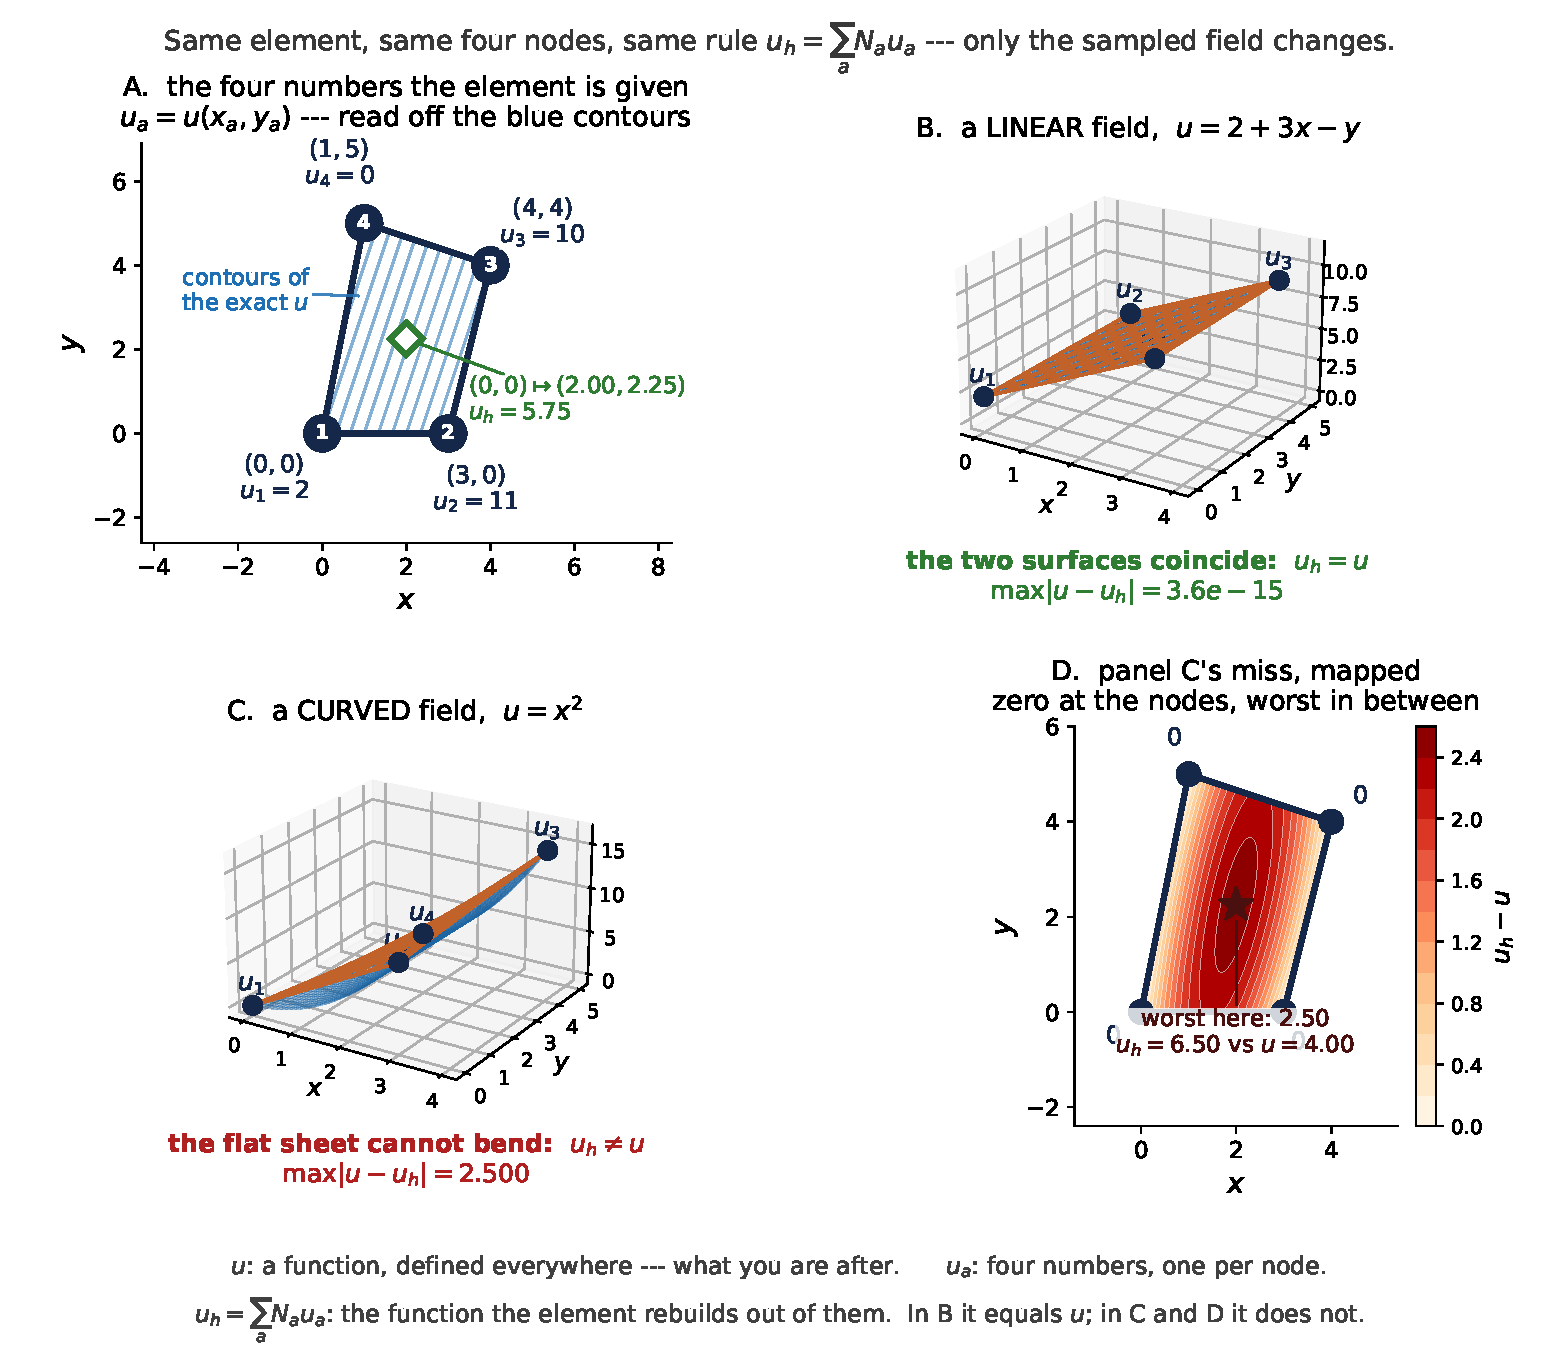
\includegraphics[width=\linewidth]{q4_three_us.pdf}
\captionof{figure}{\textbf{A:} where the four numbers come from --- the blue
contours are the exact field $u$, and $u_{a}$ is just its value read off at
node $a$. Green: the centre $(r,s)=(0,0)$, its image, and $u_{h}$ there.
\textbf{B:} the linear field of \eqref{eq:isoexact}. The blue surface is $u$,
the orange wireframe is $u_{h}$, the dots are the four $u_{a}$ --- and the two
surfaces are the \emph{same} surface, $\max|u-u_{h}|=3.6\times10^{-15}$. There
is nothing to see, which is the point. \textbf{C:} the identical element and
the identical rule, but sampling $u=x^{2}$. The four dots still sit on $u$ by
construction, yet in between the bilinear sheet cannot curve. \textbf{D:} that
miss, mapped over the element --- exactly zero at the four nodes, because the
element was \emph{told} those values, and worst in between:
$\max|u-u_{h}|=2.500$ at the centre, where $u_{h}=6.50$ against $u=4.00$.
Panels C and D are why the subscript $h$ has to exist at all. Note that the
element shape is the same in all four: distortion is not what breaks C --- the
curvature of $u$ is.}
\label{fig:threeus}
\end{center}

\outside{the six modes of a linear displacement field --- which term is which}{%
Equation \eqref{eq:isoexact} used a \emph{scalar} linear field. In 2D
elasticity the displacement has two components, so the linear field carries
\emph{six} constants --- and each one is named by the term it multiplies:
\[
\begin{aligned}
  u &=\;\; \underbrace{\alpha_{1}}_{\substack{\text{slide in }x\\ \text{\textsc{translation}}}}
   &&\;+\;\; \underbrace{\beta_{1}x}_{\substack{\text{stretch in }x\\ \varepsilon_{xx}}}
   &&\;+\;\; \underbrace{\gamma_{1}y}_{\substack{\text{tilts the}\\ \text{\textsc{vertical} edge}}}
   \\[2.8ex]
  v &=\;\; \underbrace{\alpha_{2}}_{\substack{\text{slide in }y\\ \text{\textsc{translation}}}}
   &&\;+\;\; \underbrace{\beta_{2}x}_{\substack{\text{tilts the}\\ \text{\textsc{horizontal} edge}}}
   &&\;+\;\; \underbrace{\gamma_{2}y}_{\substack{\text{stretch in }y\\ \varepsilon_{yy}}}
\end{aligned}
\]

\textbf{Four of the six read off directly.} $\alpha_{1},\alpha_{2}$ contain
no $x$ or $y$, so every point of the element gets the same push: nothing
deforms, it just slides. The \emph{diagonal} pair
$\beta_{1}=\partial u/\partial x$ and $\gamma_{2}=\partial v/\partial y$ are
the two stretches --- walk along $x$ and the $x$-displacement grows, so the
element lengthens in $x$.

\medskip
\textbf{The other two are the interesting ones.} The \emph{off-diagonal} pair
$\gamma_{1}=\partial u/\partial y$ and $\beta_{2}=\partial v/\partial x$ is
the cross-coupling: move in $y$ and get pushed sideways, move in $x$ and get
pushed up. Each one tilts a single edge of the element, and \emph{both}
rotation and shear live in that pair --- neither $\gamma_{1}$ nor $\beta_{2}$
is one or the other by itself.}

\outside{rotation vs.\ shear --- what the two tilts do together}{%
Which of the two you have depends entirely on how the tilts sit relative to
each other:
\begin{center}\small
\renewcommand{\arraystretch}{1.3}
\begin{tabular}{@{}l@{\hspace{1.3em}}l@{\hspace{1.3em}}l@{}}
\toprule
$\gamma_{1},\beta_{2}$ lean \ldots & so the element \ldots
  & and the pair is \ldots\\
\midrule
the \emph{same} rotational way & spins; the corner stays $90^{\circ}$
  & \textsc{rotation}\\
\emph{into} each other & its $90^{\circ}$ corner closes up
  & \textsc{shear}\\
\bottomrule
\end{tabular}
\end{center}
\[
  \underbrace{\gamma_{1}+\beta_{2}}_{=\,\gamma_{xy}\ \text{(shear)}}
  \qquad\qquad\qquad
  \underbrace{\beta_{2}-\gamma_{1}}_{=\,2\omega\ \text{(rotation)}}
\]
The \emph{sum} of the two tilts is the deformation; their \emph{difference}
is the spin. The one test that separates them: \emph{did the right angle
survive?} Equivalently, the displacement gradient splits once and for all
into a symmetric part and a skew part,
$\grad\bm{u}=\bm{\varepsilon}+\bm{W}$, and those are exactly strain and
rotation.

\medskip
\textbf{The count.} $2$ translation $+\ 1$ rotation $+\ 3$ constant strain
$=6$ --- precisely the six constants above, nothing left over and nothing
double-counted. The first three store no strain energy, which is why a
correctly formed $k^{e}$ has exactly three zero eigenvalues in 2D; the last
three are what the patch test demands the element reproduce exactly, and what
\eqref{eq:isoexact} guarantees it does.}

\medskip
\textbf{The one thing that can go wrong.} The map must be invertible, which
needs $J>0$ \emph{everywhere} in the element, not just at the corners. Distort
a quad far enough --- make it concave, or let two corners cross --- and $J$
changes sign, the element folds over itself, and the computed stiffness is
meaningless. This is precisely what a mesher's ``negative Jacobian'' error
reports, and it is why element-quality checks exist.

\medskip
\noindent\fbox{\parbox{0.955\linewidth}{%
\textbf{Say it in one sentence.} ``Isoparametric means the element uses the
same shape functions to describe its own geometry as it does to interpolate
the solution.''}}

\medskip
\textbf{Step (i) --- the four shape functions at $(r,s)=(0.5,0.5)$.}
From \eqref{eq:N}, substituting $r=0.5$ and $s=0.5$:
\begin{alignat}{4}
  N_{1}&=\tfrac14(1-r)(1-s)\ &&=\ \tfrac14(0.5)(0.5)\ &&=\ \tfrac{1}{16}\ &&=\ 0.0625,\notag\\
  N_{2}&=\tfrac14(1+r)(1-s)\ &&=\ \tfrac14(1.5)(0.5)\ &&=\ \tfrac{3}{16}\ &&=\ 0.1875,\notag\\
  N_{3}&=\tfrac14(1+r)(1+s)\ &&=\ \tfrac14(1.5)(1.5)\ &&=\ \tfrac{9}{16}\ &&=\ 0.5625,\notag\\
  N_{4}&=\tfrac14(1-r)(1+s)\ &&=\ \tfrac14(0.5)(1.5)\ &&=\ \tfrac{3}{16}\ &&=\ 0.1875,
  \label{eq:Nhalf}
\end{alignat}
and as a check $N_{1}+N_{2}+N_{3}+N_{4}=0.0625+0.1875+0.5625+0.1875=1$,
as \eqref{eq:pou} requires.

\medskip
\noindent
\textbf{Notice what was \emph{not} used.} Nothing in \eqref{eq:Nhalf} mentions
$D$'s corners, or its size, or where it sits. At this point the element could be
\emph{any} quadrilateral anywhere in the mesh and these four numbers would be
identical. The physical geometry has not entered yet --- and it enters only in
Steps (ii) and (iii), through the corner coordinates.

\medskip

\textbf{Step (ii) --- the $x$ coordinate.} The corner values are
$x_{1}=0$, $x_{2}=3$, $x_{3}=4$, $x_{4}=1$:
\begin{align}
  x&=N_{1}x_{1}+N_{2}x_{2}+N_{3}x_{3}+N_{4}x_{4}\notag\\
   &=0.0625\,(0)\;+\;0.1875\,(3)\;+\;0.5625\,(4)\;+\;0.1875\,(1)\notag\\
   &=0\;+\;0.5625\;+\;2.25\;+\;0.1875\notag\\
   &=3 .\label{eq:xmap}
\end{align}

\medskip
\textbf{Step (iii) --- the $y$ coordinate.} The corner values are
$y_{1}=0$, $y_{2}=0$, $y_{3}=4$, $y_{4}=5$:
\begin{align}
  y&=N_{1}y_{1}+N_{2}y_{2}+N_{3}y_{3}+N_{4}y_{4}\notag\\
   &=0.0625\,(0)\;+\;0.1875\,(0)\;+\;0.5625\,(4)\;+\;0.1875\,(5)\notag\\
   &=0\;+\;0\;+\;2.25\;+\;0.9375\notag\\
   &=3.1875 .\label{eq:ymap}
\end{align}

\medskip
So $(r,s)=(0.5,0.5)$ sits at the physical point $(3,\,3.1875)$ --- the entry
in row $D$ of Table~\ref{tab:why}.
And $N_{3}$ itself is \emph{unchanged} at $0.5625$ --- because $N_{3}$ is a
function of $(r,s)$ alone and never sees the element's shape. For $A$, $B$ and
$C$ the reference square is a convenience; for $D$ it is the only thing that
works.

% ------------------------------------------------------------------
\subsubsection*{What the $x,y$ coordinates are \emph{for}}

The physical description of an element carries exactly three things:

\begin{center}\small
\renewcommand{\arraystretch}{1.25}
\begin{tabular}{@{}ll@{}}
\toprule
\textbf{location} & where the element sits in the mesh\\
\textbf{size} & how big it is\\
\textbf{shape} & its aspect ratio and distortion\\
\bottomrule
\end{tabular}
\end{center}

\noindent
Those three are the \emph{only} things that tell one element from another, and
they are the only reason the ``$N_{3}$ in $x,y$'' column of
Table~\ref{tab:why} changed from row to row. The reference square carries
\textbf{none} of them: in $(r,s)$ every element in the mesh is literally the
same square, and $N_{1},\dots,N_{4}$ cannot tell them apart.

\medskip
So where did location, size and shape go? Into the map --- and from the map
into exactly two places:

\begin{steps}
\item \textbf{The corner coordinates $x_{a},y_{a}$}, used by
      $x=\sum_{a}N_{a}x_{a}$ whenever an actual physical position is wanted.
      That is all of Steps (ii) and (iii), and nothing else needs them.
\item \textbf{The Jacobian $J$}, which carries size and shape into every
      integral and every derivative:
\begin{equation}\label{eq:jac}
  \mathrm{d}\Omega=|J|\,\mathrm{d}r\,\mathrm{d}s,
  \qquad
  \frac{\partial N_{a}}{\partial x}
   =\frac{\partial N_{a}}{\partial r}\frac{\partial r}{\partial x}
   +\frac{\partial N_{a}}{\partial s}\frac{\partial s}{\partial x} .
\end{equation}
\end{steps}

\noindent
And $J$ is where the difference between a tidy element and a distorted one
actually shows up:
\begin{equation}\label{eq:jacvals}
  \text{rectangle } a\times b:\quad J=\frac{ab}{4}\ \ \text{(constant)},
  \qquad
  \text{element } D:\quad J=\frac54+\frac{r}{8}-\frac{s}{4}\ \ \text{(varies)} .
\end{equation}
For the rectangle $J$ is one number for the whole element --- which is why
\eqref{eq:ke} came out in closed form. For $D$ it ranges from $3$ to
$4$ across the four corners, so it must be re-evaluated at every quadrature
point. (Integrating it recovers the area: $\int_{-1}^{1}\!\int_{-1}^{1}J\,
\mathrm{d}r\,\mathrm{d}s=14$, which is the area of $D$.)

\medskip
\noindent\fbox{\parbox{0.955\linewidth}{%
\textbf{The division of labour.} $(r,s)$ holds the \emph{interpolation} --- how
the four nodal values are blended, identical for every element. $x,y$ holds the
\emph{geometry} --- location, size, shape, compressed into the corner
coordinates and the Jacobian. The two meet only inside the integral, and
nowhere else.}}

% ------------------------------------------------------------------
\subsubsection*{The map only runs one way --- and that is all that is needed}

Notice the asymmetry in what was just done. Given $(r,s)$, the four
contributions $N_{1},N_{2},N_{3},N_{4}$ are known \emph{immediately} ---
\eqref{eq:Nhalf} is substitution, nothing more --- and the physical point
follows by \eqref{eq:xmap}--\eqref{eq:ymap}. Going the other way is not like
that at all. For element $D$ the forward map is
\begin{equation}\label{eq:fwdD}
  x(r,s)=2+\tfrac32 r+\tfrac12 s,
  \qquad
  y(r,s)=\tfrac94-\tfrac14 r+\tfrac94 s-\tfrac14 rs ,
\end{equation}
so recovering $(r,s)$ from a given $(x,y)$ means solving \emph{two coupled
nonlinear equations} --- there is an $rs$ term, so the system is not linear.
Eliminating $r$ leaves a \textbf{quadratic} in $s$, and a quadratic has two
roots. For the point $(3,\,3.1875)$ they are
\begin{equation}\label{eq:invD}
  (r,s)=\Bigl(\tfrac12,\tfrac12\Bigr)\ \ \text{\cmark\ inside } [-1,1]^{2},
  \qquad
  (r,s)=\Bigl(\tfrac{19}{2},-\tfrac{53}{2}\Bigr)\ \ \text{\xmark\ outside --- discard} .
\end{equation}
So the inverse exists here, but it costs a quadratic solve \emph{and} a test to
throw away the spurious root. For a curved or three-dimensional element there
is no closed form at all and one iterates with Newton's method.

\medskip
\noindent\fbox{\parbox{0.955\linewidth}{%
\textbf{Why this does not matter.} The finite element method never asks the
inverse question. Every quantity it needs is an \emph{integral over the
element}, and \eqref{eq:keint} turns each one into an integral over the
reference square: you place Gauss points in $(r,s)$, evaluate
$N_{a}$ and its derivatives there, and map \emph{forward} to $(x,y)$ only if
the integrand needs it. The traffic is one-way by construction, which is
exactly why only the easy direction was ever built.}}

\medskip
{\small\color{black!60}The one place the inverse does come up is
post-processing: ``what is the solution at this particular physical point?''
--- for a sensor location, say. A code answers it by finding which element
contains the point and then inverting the map numerically, which is why probing
an arbitrary point is more expensive than reading a nodal value, where the
answer is just $\xi_{j}$.}

\medskip
\noindent
\noindent\fbox{\parbox{0.955\linewidth}{%
\textbf{Read the number correctly.} $N_{3}$ belongs to \textbf{node $3$} --- the
subscript names a \emph{node}, never a point. Evaluating it somewhere returns
the \emph{weight that node $3$'s value carries at that location}:
\[
  u_{h}(P)=N_{1}(P)\,u_{1}+N_{2}(P)\,u_{2}
          +\underbrace{N_{3}(P)\,u_{3}}_{\text{node 3's share}}+N_{4}(P)\,u_{4}.
\]
So the $0.5625$ in Table~\ref{tab:why} is not ``the value of $N_{3}$ at
$(0.5,0.5)$'' as though it were a property of that point --- it is \emph{how
much node $3$ contributes there}. On element $B$, node~$3$ sits physically at
$(3,2)$ and contributes $0.5625$ to the point $(2.50,1.50)$. Which node a
shape function belongs to is fixed; changing between $x,y$ and $(r,s)$ only
changes the coordinates used to \emph{locate} the evaluation point.}}

\medskip
\noindent
In Table~\ref{tab:why} the region, the $x,y$ formula and both ``sits at''
columns change from element to element; the two share columns do not. As
counted above, a mesh of $10{,}000$ elements would need $40{,}000$ formulas in
$x,y$ and needs exactly \textbf{four} in $(r,s)$. Everything about where the
element is and how big it is has moved out of the shape functions and into the
map. Three consequences:

\begin{steps}
\item \textbf{You write the formulas once.} \eqref{eq:N} is hard-coded in the
      program. Nothing about it changes from element to element, or from mesh
      to mesh.
\item \textbf{Every integral gets the same limits.} The element matrix
      \eqref{eq:keint} becomes
      $\int_{-1}^{1}\!\int_{-1}^{1}(\cdots)\,|J|\,\mathrm{d}r\,\mathrm{d}s$ for
      \emph{every} element, so one fixed Gauss rule --- the same points, the
      same weights --- integrates the whole mesh. Working in $x,y$ you would
      need a different set of quadrature points for every element.
\item \textbf{It is the only practical route for element $D$.} For four
      arbitrary corners the bilinear function in $x,y$ has no tidy closed form,
      but the map still works: use the \emph{same} $N_{a}$ to carry the
      geometry, $x(r,s)=\sum_{a}N_{a}(r,s)\,x_{a}$ and
      $y(r,s)=\sum_{a}N_{a}(r,s)\,y_{a}$. That is what
      \textbf{isoparametric} means --- same shapes for the geometry as for the
      unknown --- and it is why real meshes may use distorted quads at all.
\end{steps}

\medskip
{\small\color{black!60}Put the other way round: the reference square is a change
of variables, nothing deeper. It does not alter $\varphi_{j}$ or the method ---
\eqref{eq:fourterms} is still what is being computed. It only spares you from
re-deriving the same four polynomials once per element.}

% ------------------------------------------------------------------
\subsection*{Step 4 --- this is where $\varphi$ becomes $N$}

\medskip\noindent\fbox{\parbox{0.955\linewidth}{%
\textbf{Definition.} $N_{a}$ is the global basis function $\varphi_{j}$,
restricted to one element, and rewritten in the reference coordinates:
\[
  N_{a}(r,s)\;\coloneqq\;\varphi_{j}\big|_{K}\bigl(x(r,s),\,y(r,s)\bigr),
  \qquad a=\text{local number of global node } j \text{ in } K .
\]
That is the whole of it. $N$ is not a new object --- it is $\varphi$ seen on
one element, in borrowed coordinates.}}

\medskip
And the nodal condition comes along with it. Restrict \eqref{eq:globaldelta} to
$K$'s own four corners: $\varphi_{j}$ is $1$ at its own corner and $0$ at the
other three, so in reference coordinates
\begin{equation}\label{eq:delta}
  \boxed{\;N_{a}(\text{node } b)=\delta_{ab},\qquad a,b=1,2,3,4\;}
\end{equation}
which is \eqref{eq:globaldelta} with the sum over $M$ global nodes narrowed to
the $4$ local ones.

% ------------------------------------------------------------------
\subsection*{Step 5 --- now solve for the four $N$'s}

By Step 2 each $N_{a}$ is bilinear, so write
\begin{equation}\label{eq:Ngen}
  N(r,s)=c_{0}+c_{1}r+c_{2}s+c_{3}\,rs ,
\end{equation}
and evaluate at the four corners $(-1,-1)$, $(1,-1)$, $(1,1)$, $(-1,1)$:
\begin{equation}\label{eq:4eqs}
\begin{aligned}
  N(-1,-1)&=c_{0}-c_{1}-c_{2}+c_{3},&\qquad
  N(1,-1)&=c_{0}+c_{1}-c_{2}-c_{3},\\
  N(1,1)&=c_{0}+c_{1}+c_{2}+c_{3},&\qquad
  N(-1,1)&=c_{0}-c_{1}+c_{2}-c_{3}.
\end{aligned}
\end{equation}
Setting these equal to the values demanded by \eqref{eq:delta} gives four
linear systems, one per node.

\medskip
\textbf{Node 1:} $N_{1}=1$ at node 1, $0$ at nodes 2, 3, 4.
\begin{equation}\label{eq:sys1}
\left\{
\begin{alignedat}{5}
  c_{0}&{}-{}&c_{1}&{}-{}&c_{2}&{}+{}&c_{3}&{}={}&1\\
  c_{0}&{}+{}&c_{1}&{}-{}&c_{2}&{}-{}&c_{3}&{}={}&0\\
  c_{0}&{}+{}&c_{1}&{}+{}&c_{2}&{}+{}&c_{3}&{}={}&0\\
  c_{0}&{}-{}&c_{1}&{}+{}&c_{2}&{}-{}&c_{3}&{}={}&0
\end{alignedat}
\right.
\qquad\Longrightarrow\qquad
c_{0}=\tfrac14,\ c_{1}=-\tfrac14,\ c_{2}=-\tfrac14,\ c_{3}=\tfrac14 ,
\end{equation}
\[
  N_{1}=\tfrac14\bigl(1-r-s+rs\bigr)=\tfrac14(1-r)(1-s).
\]

\medskip
\textbf{Node 2:} $N_{2}=1$ at node 2, $0$ at nodes 1, 3, 4.
\begin{equation}\label{eq:sys2}
\left\{
\begin{alignedat}{5}
  c_{0}&{}-{}&c_{1}&{}-{}&c_{2}&{}+{}&c_{3}&{}={}&0\\
  c_{0}&{}+{}&c_{1}&{}-{}&c_{2}&{}-{}&c_{3}&{}={}&1\\
  c_{0}&{}+{}&c_{1}&{}+{}&c_{2}&{}+{}&c_{3}&{}={}&0\\
  c_{0}&{}-{}&c_{1}&{}+{}&c_{2}&{}-{}&c_{3}&{}={}&0
\end{alignedat}
\right.
\qquad\Longrightarrow\qquad
c_{0}=\tfrac14,\ c_{1}=\tfrac14,\ c_{2}=-\tfrac14,\ c_{3}=-\tfrac14 ,
\end{equation}
\[
  N_{2}=\tfrac14\bigl(1+r-s-rs\bigr)=\tfrac14(1+r)(1-s).
\]

\medskip
\textbf{Node 3:} $N_{3}=1$ at node 3, $0$ at nodes 1, 2, 4.
\begin{equation}\label{eq:sys3}
\left\{
\begin{alignedat}{5}
  c_{0}&{}-{}&c_{1}&{}-{}&c_{2}&{}+{}&c_{3}&{}={}&0\\
  c_{0}&{}+{}&c_{1}&{}-{}&c_{2}&{}-{}&c_{3}&{}={}&0\\
  c_{0}&{}+{}&c_{1}&{}+{}&c_{2}&{}+{}&c_{3}&{}={}&1\\
  c_{0}&{}-{}&c_{1}&{}+{}&c_{2}&{}-{}&c_{3}&{}={}&0
\end{alignedat}
\right.
\qquad\Longrightarrow\qquad
c_{0}=\tfrac14,\ c_{1}=\tfrac14,\ c_{2}=\tfrac14,\ c_{3}=\tfrac14 ,
\end{equation}
\[
  N_{3}=\tfrac14\bigl(1+r+s+rs\bigr)=\tfrac14(1+r)(1+s).
\]

\medskip
\textbf{Node 4:} $N_{4}=1$ at node 4, $0$ at nodes 1, 2, 3.
\begin{equation}\label{eq:sys4}
\left\{
\begin{alignedat}{5}
  c_{0}&{}-{}&c_{1}&{}-{}&c_{2}&{}+{}&c_{3}&{}={}&0\\
  c_{0}&{}+{}&c_{1}&{}-{}&c_{2}&{}-{}&c_{3}&{}={}&0\\
  c_{0}&{}+{}&c_{1}&{}+{}&c_{2}&{}+{}&c_{3}&{}={}&0\\
  c_{0}&{}-{}&c_{1}&{}+{}&c_{2}&{}-{}&c_{3}&{}={}&1
\end{alignedat}
\right.
\qquad\Longrightarrow\qquad
c_{0}=\tfrac14,\ c_{1}=-\tfrac14,\ c_{2}=\tfrac14,\ c_{3}=-\tfrac14 ,
\end{equation}
\[
  N_{4}=\tfrac14\bigl(1-r+s-rs\bigr)=\tfrac14(1-r)(1+s).
\]

\medskip
Collecting the four:

\begin{equation}\label{eq:N}
  \boxed{\;
  \begin{aligned}
    N_{1}(r,s)&=\tfrac14(1-r)(1-s), &\qquad N_{2}(r,s)&=\tfrac14(1+r)(1-s),\\[2pt]
    N_{3}(r,s)&=\tfrac14(1+r)(1+s), &\qquad N_{4}(r,s)&=\tfrac14(1-r)(1+s).
  \end{aligned}\;}
\end{equation}

\medskip
There is a shortcut worth seeing, because it explains the product form: each
$N_{a}$ must vanish on the \emph{two edges} not touching node $a$. Those edges
are $r=\mp1$ and $s=\mp1$, so $N_{a}$ must contain both factors; normalise by
dividing by its value at its own node, which is $4$. That is \eqref{eq:N}
without solving anything. A compact way to write all four:
\begin{equation}\label{eq:Ncompact}
  N_{a}(r,s)=\tfrac14\bigl(1+r_{a}r\bigr)\bigl(1+s_{a}s\bigr),
  \qquad (r_{a},s_{a})=\text{coordinates of node } a .
\end{equation}

\begin{center}
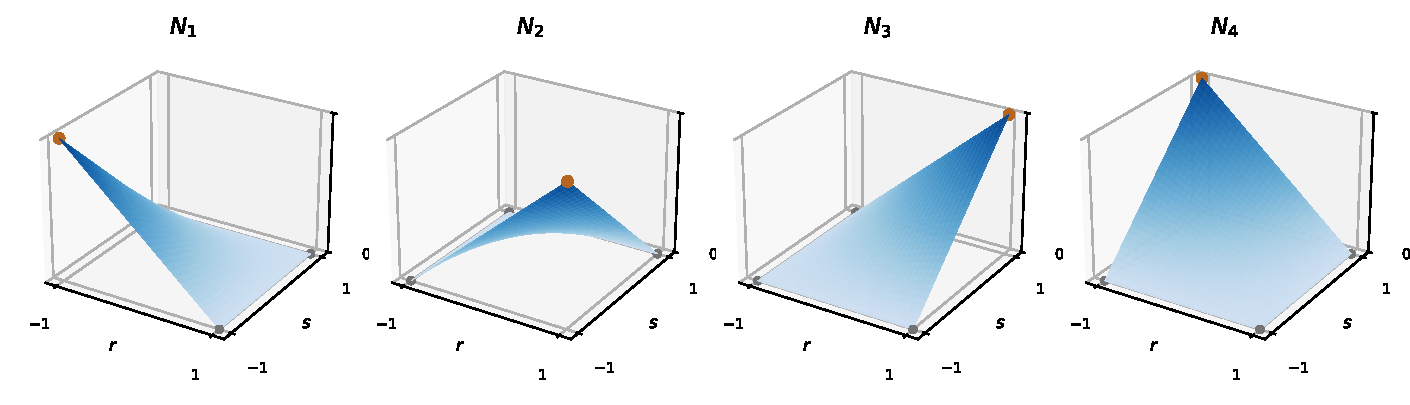
\includegraphics[width=\linewidth]{q4_shapes.pdf}
\captionof{figure}{The four bilinear shape functions on the reference square. Each is
$1$ at its own node (orange) and $0$ at the other three (grey) --- which is
exactly \eqref{eq:delta}, the lecture's nodal table written for a quadrilateral.}
\label{fig:shapes}
\end{center}

\begin{center}
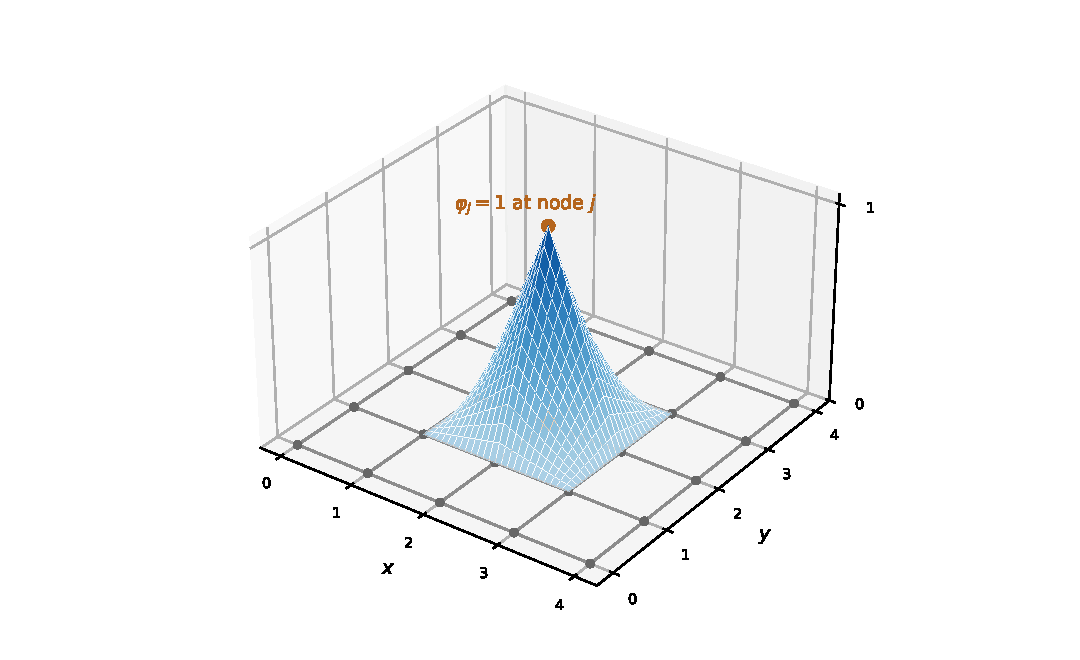
\includegraphics[width=0.92\linewidth]{q4_hat_on_mesh.pdf}
\captionof{figure}{The same four shapes, assembled. On the $16$-element mesh of
\S3 Step~1 ($5\times5=25$ nodes), the global basis function $\varphi_{j}$ is a
\textbf{hat} standing on exactly four elements and flat --- identically zero ---
on the other twelve. Its four faces are $N_{3},N_{4},N_{2},N_{1}$ of those four
elements, which is \eqref{eq:phiexplicit} drawn. This is the object the
lecturer means by $\varphi_{j}$; the four panels of Figure~\ref{fig:shapes}
are the pieces it is cut from.}
\label{fig:hat}
\end{center}

\textbf{Two identities that follow immediately} (both verified symbolically):
\begin{align}
  \sum_{a=1}^{4}N_{a}(r,s)&=1 &&\text{(partition of unity)},\label{eq:pou}\\
  \sum_{a=1}^{4}N_{a}(r,s)\,r_{a}=r,\qquad
  \sum_{a=1}^{4}N_{a}(r,s)\,s_{a}&=s &&\text{(linear fields reproduced exactly)}.
  \label{eq:lin}
\end{align}
\eqref{eq:pou} is the rigid-body (constant) mode: a uniform nodal value gives a
uniform field. \eqref{eq:lin} is the constant-gradient mode. Together they are
the patch test, and they are why the element converges at all --- without them
$\norm{u-\Pi_{h}u}\not\to0$ and C\'ea's lemma delivers nothing.

% ==================================================================
\section*{4. $\varphi$ versus $N$: the picture}

$N_{a}$ lives on \textbf{one element}, in local coordinates. The lecture's
$\varphi_{j}$ lives on \textbf{all of $\Omega$}, in global coordinates, one per
global node. The relation:

\medskip
\noindent\fbox{\parbox{0.955\linewidth}{\centering
$\varphi_{j}$ restricted to element $e$ $\;=\;$ $N_{a}$,
\ \ where $a$ is the \emph{local} number of global node $j$ inside $e$.}}

\medskip
In a structured quad mesh an interior node belongs to $4$ elements, so
$\varphi_{j}$ is $4$ local $N$'s glued together, and zero everywhere else.

\begin{center}
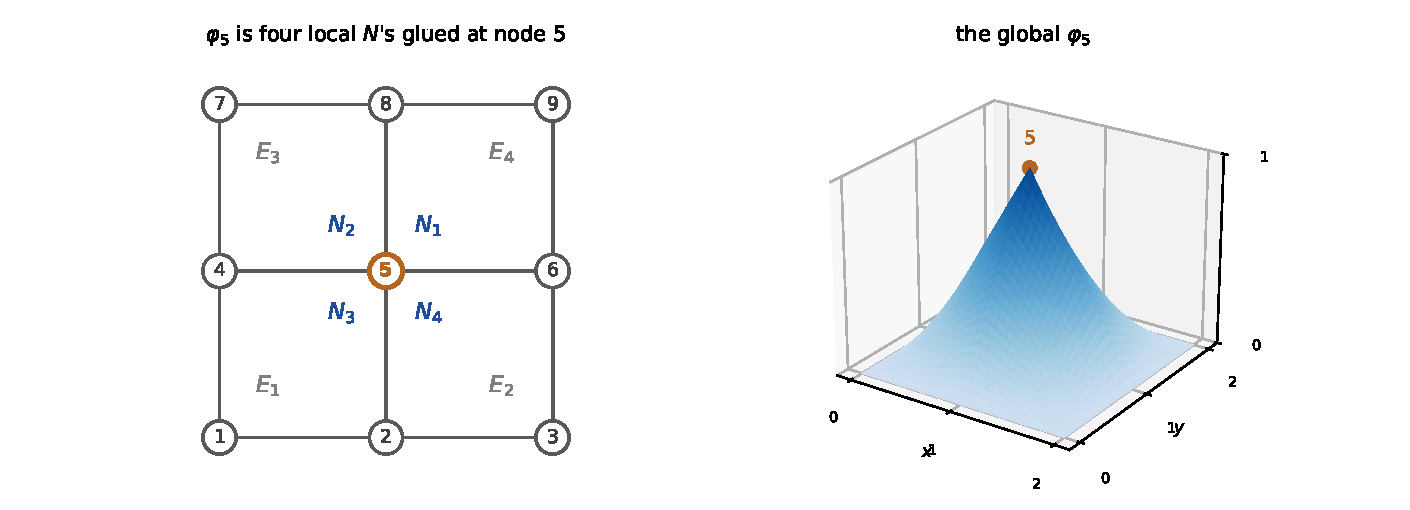
\includegraphics[width=\linewidth]{q4_global_phi.pdf}
\captionof{figure}{Left: node $j$ is shared by four elements, and in each one it carries a
different \emph{local} number --- so $\varphi_{j}$ is built from $N_{3}$, $N_{4}$,
$N_{2}$, $N_{1}$ of those four elements respectively. Right: the resulting
$\varphi_{j}$, the function the lecturer actually means.}
\label{fig:glue}
\end{center}

% ------------------------------------------------------------------
\subsection*{Writing that $\varphi$ out explicitly}

Take the patch in Figure~\ref{fig:glue}: four unit squares on $[0,2]^{2}$, node $5$ at the
centre $(1,1)$. Each element maps to the reference square by
$r=2(x-x_{e})-1$, $s=2(y-y_{e})-1$, where $(x_{e},y_{e})$ is its lower-left
corner. Substituting that into the $N$ named in each quadrant:

\begin{center}\small
\renewcommand{\arraystretch}{1.45}
\begin{tabular}{@{}llcl@{}}
\toprule
element & region & node 5 is local & $\varphi_{5}$ there\\
\midrule
$E_{1}$ & $[0,1]\times[0,1]$ & $3$ & $N_{3}=\tfrac14(1+r)(1+s)
   \;\xrightarrow{\;r=2x-1,\ s=2y-1\;}\; \bm{xy}$\\
$E_{2}$ & $[1,2]\times[0,1]$ & $4$ & $N_{4}=\tfrac14(1-r)(1+s)
   \;\xrightarrow{\;r=2x-3,\ s=2y-1\;}\; \bm{(2-x)\,y}$\\
$E_{3}$ & $[0,1]\times[1,2]$ & $2$ & $N_{2}=\tfrac14(1+r)(1-s)
   \;\xrightarrow{\;r=2x-1,\ s=2y-3\;}\; \bm{x\,(2-y)}$\\
$E_{4}$ & $[1,2]\times[1,2]$ & $1$ & $N_{1}=\tfrac14(1-r)(1-s)
   \;\xrightarrow{\;r=2x-3,\ s=2y-3\;}\; \bm{(2-x)(2-y)}$\\
\bottomrule
\end{tabular}
\captionof{table}{$\varphi_{5}$ written out on each of the four elements of Figure~\ref{fig:glue}.}
\label{tab:phi5}
\end{center}

\noindent
so the global basis function of node $5$ is, in one piece,
\begin{equation}\label{eq:phiexplicit}
  \boxed{\;
  \varphi_{5}(x,y)=
  \begin{cases}
    x\,y, & 0\le x\le1,\ 0\le y\le1 \quad (E_{1}),\\[2pt]
    (2-x)\,y, & 1\le x\le2,\ 0\le y\le1 \quad (E_{2}),\\[2pt]
    x\,(2-y), & 0\le x\le1,\ 1\le y\le2 \quad (E_{3}),\\[2pt]
    (2-x)(2-y), & 1\le x\le2,\ 1\le y\le2 \quad (E_{4}),\\[2pt]
    0, & \text{everywhere else.}
  \end{cases}\;}
\end{equation}

\noindent
Equivalently, in closed form, $\varphi_{5}(x,y)=\hat{h}(x-1)\,\hat{h}(y-1)$ with
$\hat{h}(t)=\max(0,1-|t|)$ --- a product of two 1D hats. (Checked: the four
pieces agree with this at interior sample points.)

\medskip
\textbf{Two things to read off \eqref{eq:phiexplicit}.}
\begin{steps}
\item \textbf{It is continuous, so $\varphi_{5}\in H^{1}$.} Across the interior
      edge $x=1$: from $E_{1}$ it is $xy\to y$, from $E_{2}$ it is
      $(2-x)y\to y$. Equal. Likewise across $y=1$. This is the $C^{0}$
      conformity of \S2, now visible as algebra.
\item \textbf{Its gradient jumps, and that is allowed.} At $x=1$,
      $\partial_{x}\varphi_{5}=y$ from the left and $-y$ from the right --- a
      jump of $2y$. The lecture only ever required
      $\iint\|\grad v\|^{2}<\infty$, and a finite jump is square integrable.
      A jump in $\varphi$ itself would not be.
\item Each piece is a different formula, which is the practical reason nobody
      assembles $\varphi$ --- whereas the four $N_{a}$ in \eqref{eq:N} are the
      same for every element in the mesh.
\end{steps}

\medskip
{\small\color{black!60}In practice you never build the right-hand picture of
Figure~\ref{fig:glue}, nor \eqref{eq:phiexplicit}. You loop over elements and use the
left-hand one. The $\varphi_{j}$ exists only implicitly, inside the
connectivity table --- which is the honest answer to ``where is $\varphi$ in my
code?''\ \ It is the \texttt{IEN}/\texttt{LM} array.}

% ==================================================================
\section*{5. Worked example: a mesh with four elements}

Everything above is one element. Here is what $\varphi$ and $N$ actually
\emph{equal}, as numbers, when there is more than one.

\medskip
\textbf{The mesh.} Four unit squares on $[0,2]\times[0,2]$: $9$ global nodes,
$4$ elements. Global node numbers are circled, element numbers are in the
centres, and the orange dot is the point
\[
  P=(1.3,\ 0.4)
\]
at which we will evaluate everything.

\begin{center}
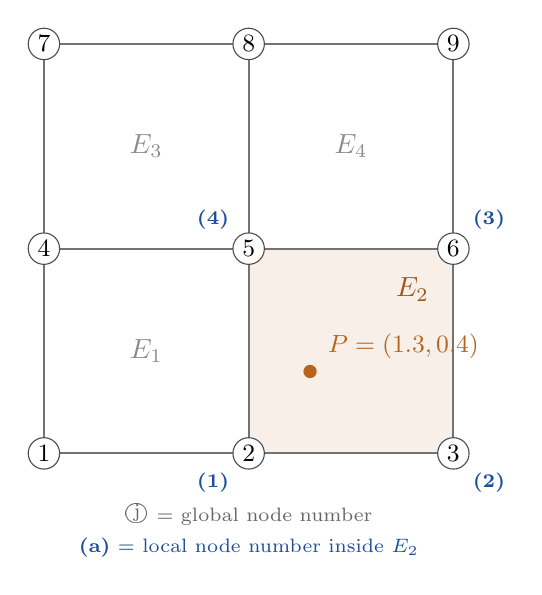
\begin{tikzpicture}[x=2.6cm,y=2.6cm,>=latex]
  % shade the element containing P
  \fill[EngC!10] (1,0) rectangle (2,1);
  % grid
  \foreach \k in {0,1,2}{
    \draw[black!55,thick] (0,\k) -- (2,\k);
    \draw[black!55,thick] (\k,0) -- (\k,2);}
  % element labels
  \node[black!45] at (0.5,0.5) {$E_{1}$};
  \node[EngC!85!black] at (1.80,0.80) {$E_{2}$};
  \node[black!45] at (0.5,1.5) {$E_{3}$};
  \node[black!45] at (1.5,1.5) {$E_{4}$};
  % global nodes
  \foreach \x/\y/\n in {0/0/1, 1/0/2, 2/0/3, 0/1/4, 1/1/5, 2/1/6,
                        0/2/7, 1/2/8, 2/2/9}{
    \node[circle,draw=black!70,fill=white,inner sep=1.4pt,font=\small]
      at (\x,\y) {\n};}
  % local numbering inside E2
  \foreach \x/\y/\a/\pos in {1/0/1/{below left}, 2/0/2/{below right},
                             2/1/3/{above right}, 1/1/4/{above left}}{
    \node[font=\scriptsize,text=MathC,\pos=5pt] at (\x,\y) {\textbf{(\a)}};}
  % the point P
  \fill[EngC] (1.3,0.4) circle (2.4pt);
  \node[font=\small,text=EngC,above right=1pt and 3pt] at (1.3,0.4) {$P=(1.3,0.4)$};
  % legend, two clear lines below the mesh
  \node[font=\scriptsize,text=black!60] at (1,-0.30)
    {\raisebox{1pt}{\textcircled{\scriptsize j}} $=$ global node number};
  \node[font=\scriptsize,text=MathC] at (1,-0.46)
    {\textbf{(a)} $=$ local node number inside $E_{2}$};
\end{tikzpicture}
\end{center}

% ------------------------------------------------------------------
\subsection*{(a) The $\varphi$ values --- nine numbers, five of them zero}

Each global $\varphi_{j}$ is the product of two $1$D hats,
$\varphi_{j}(x,y)=\hat{h}(x-x_{j})\,\hat{h}(y-y_{j})$ with
$\hat{h}(t)=\max(0,1-|t|)$. Evaluating all nine at $P=(1.3,0.4)$:

\begin{center}\small
\renewcommand{\arraystretch}{1.25}
\begin{tabular}{@{}cccl@{}}
\toprule
global node $j$ & position & $\varphi_{j}(P)$ & \\
\midrule
$1$ & $(0,0)$ & $0$ & \color{black!50}$P$ is more than one element away\\
$2$ & $(1,0)$ & $\bm{0.42}$ & \\
$3$ & $(2,0)$ & $\bm{0.18}$ & \\
$4$ & $(0,1)$ & $0$ & \color{black!50}\\
$5$ & $(1,1)$ & $\bm{0.28}$ & \\
$6$ & $(2,1)$ & $\bm{0.12}$ & \\
$7$ & $(0,2)$ & $0$ & \color{black!50}\\
$8$ & $(1,2)$ & $0$ & \color{black!50}\\
$9$ & $(2,2)$ & $0$ & \color{black!50}\\
\midrule
 & & $\sum=1.00$ & \color{black!50}partition of unity, \eqref{eq:pou}\\
\bottomrule
\end{tabular}
\captionof{table}{All nine $\varphi_{j}$ evaluated at $P=(1.3,0.4)$. Only the four corners of the element containing $P$ are non-zero.}
\label{tab:phivals}
\end{center}

\textbf{Read this off the sketch.} The only non-zero $\varphi$'s are those of
nodes $2,3,6,5$ --- exactly \textbf{the four corners of the shaded element
$E_{2}$}, the one containing $P$. Every other node is too far away: its hat has
already fallen to zero before reaching $P$. That is ``small support'', in
numbers.

% ------------------------------------------------------------------
\subsection*{(b) The $N$ values --- four numbers, in element $E_{2}$ only}

$E_{2}$ spans $x\in[1,2]$, $y\in[0,1]$, so the map to the reference square is
$r=2x-3$, $s=2y-1$, giving at $P$
\[
  r=2(1.3)-3=-0.40,\qquad s=2(0.4)-1=-0.20 .
\]
Substituting into \eqref{eq:N}:
\begin{align*}
  N_{1}&=\tfrac14(1-r)(1-s)=\tfrac14(1.4)(1.2)=\bm{0.42},&
  N_{2}&=\tfrac14(1+r)(1-s)=\tfrac14(0.6)(1.2)=\bm{0.18},\\
  N_{3}&=\tfrac14(1+r)(1+s)=\tfrac14(0.6)(0.8)=\bm{0.12},&
  N_{4}&=\tfrac14(1-r)(1+s)=\tfrac14(1.4)(0.8)=\bm{0.28},
\end{align*}
and again $\sum_{a}N_{a}=1.00$.

% ------------------------------------------------------------------
\subsection*{(c) They are the same four numbers}

The connectivity of $E_{2}$ --- the blue \textbf{(a)} labels in the sketch ---
is local $1,2,3,4\ \mapsto$ global $2,3,6,5$. Lining the two tables up:

\begin{center}\small
\renewcommand{\arraystretch}{1.3}
\begin{tabular}{@{}ccccc@{}}
\toprule
local $a$ & global $j$ & $N_{a}(r,s)$ & $\varphi_{j}(P)$ & \\
\midrule
$1$ & $2$ & $0.42$ & $0.42$ & \cmark\\
$2$ & $3$ & $0.18$ & $0.18$ & \cmark\\
$3$ & $6$ & $0.12$ & $0.12$ & \cmark\\
$4$ & $5$ & $0.28$ & $0.28$ & \cmark\\
\bottomrule
\end{tabular}
\captionof{table}{The four $N$ values and the four non-zero $\varphi$ values are the same numbers, matched by the connectivity.}
\label{tab:match}
\end{center}

\medskip
\noindent\fbox{\parbox{0.955\linewidth}{%
\textbf{So, to answer the question directly.} With several elements:
\begin{itemize}[leftmargin=1.3em,topsep=3pt,itemsep=3pt]
\item There are \mth{$M=9$ functions $\varphi_{j}$}, one per global node, each
      defined over the \emph{whole} mesh. At any given point, \textbf{at most
      four are non-zero} --- the corners of the element you are standing in.
\item There are \eng{$4$ functions $N_{a}$}, defined only on the reference
      square, and \textbf{the same four formulas are reused for every element}
      in the mesh.
\item At a point inside element $e$, the four non-zero $\varphi$ values
      \emph{are} the four $N$ values, matched up by the connectivity table.
\end{itemize}
$\varphi$ is one function per unknown spread over the mesh; $N$ is one formula
per corner reused everywhere. Same numbers.}}

\medskip
{\small\color{black!60}This is also why $\bm{K}$ is sparse. $A_{ij}$ is
non-zero only when $\varphi_{i}$ and $\varphi_{j}$ overlap, \ie\ when nodes $i$
and $j$ share an element. In the sketch, node $1$ and node $9$ never share one,
so $A_{1,9}=0$ --- without computing anything.}

% ==================================================================
\section*{6. Why each side uses what it uses}

The two views are not a matter of taste. Each is the only one that works for
what that side needs to do.

% ------------------------------------------------------------------
\subsection*{Why the mathematician insists on $\varphi$}

\begin{steps}
\item The weak form $\displaystyle\iint_{\Omega}\grad u\cdot\grad v\dOm$ is
      \textbf{one integral over $\Omega$}, and $V_{h}$ is \textbf{one space}.
\item Every theorem in the course is a statement about \emph{functions on
      $\Omega$}, not about elements:
      \begin{center}\small
      \renewcommand{\arraystretch}{1.25}
      \begin{tabular}{@{}ll@{}}
      \toprule
      statement & what it quantifies over\\
      \midrule
      $u_{h}\in V_{h}$ & a single function on all of $\Omega$\\
      Galerkin orthogonality $B(u-u_{h},v)=0\ \forall v\in V_{h}$ & every $v$ in the whole space\\
      C\'ea $\norm{u-u_{h}}\le\frac{\beta^{*}}{\beta_{*}}\norm{u-v}$ & norms over all of $\Omega$\\
      Lax--Milgram & existence/uniqueness in $V$\\
      \bottomrule
      \end{tabular}
      \end{center}
\item \textbf{You cannot even write ``$u_{h}\in V_{h}$'' in local coordinates.}
      $N_{a}(r,s)$ is defined on $[-1,1]^{2}$; it is not a function on
      $\Omega$ at all until you say \emph{which element} and compose with the
      map. Conformity, $V_{h}\subset V$, is a statement about continuity
      \emph{between} elements --- precisely the thing local coordinates cannot
      see.
\end{steps}

% ------------------------------------------------------------------
\subsection*{Why the engineer never builds $\varphi$}

\begin{steps}
\item You loop over elements, compute $\bm{k}^{e}$ from the $N$'s, and scatter
      into $\bm{K}$. At no point is a global $\varphi_{j}$ ever formed.
\item It would be wasteful: $\varphi_{j}$ is zero on all but $4$ of the
      thousands of elements, so assembling it explicitly means storing and
      integrating mostly zeros.
\item It would also be awkward: $\varphi_{j}$ has a different algebraic
      expression on each of its four elements, whereas $N_{a}(r,s)$ is the
      \emph{same} four formulas for every element in the mesh. All the geometry
      is pushed into the Jacobian.
\item \textbf{So where is $\varphi$ in the code?} In the connectivity table ---
      the \texttt{IEN}/\texttt{LM} array. The statement ``global node $j$ is
      local node $a$ of element $e$'' \emph{is} the statement
      $\varphi_{j}|_{K_{e}}=N_{a}$. The array is the only place $\varphi$ is
      recorded, and it is recorded as an integer.
\end{steps}

% ------------------------------------------------------------------
\subsection*{The identity that makes both legal}

The two views meet in one equation. Start from the lecture's definition,
\begin{equation}\label{eq:Aij}
  A_{ij}=B(\varphi_{i},\varphi_{j})
        =\iint_{\Omega}\grad\varphi_{i}\cdot\grad\varphi_{j}\dOm ,
\end{equation}
and split the integral element by element --- legal because
$\Omega=\bigcup_{e}K_{e}$ and the elements overlap only on edges, which have
zero area:
\begin{equation}\label{eq:assembly}
  \boxed{\;
  A_{ij}=\sum_{e}\ \iint_{K_{e}}\grad\varphi_{i}\cdot\grad\varphi_{j}\dOm
        =\sum_{e}\ \underbrace{\iint_{K_{e}}\grad N_{a}\cdot\grad N_{b}\dOm}
                              _{\textstyle k^{e}_{ab}}\;}
\end{equation}
where $a,b$ are the local numbers of global nodes $i,j$ in element $e$, and the
term is simply absent if either node does not belong to $e$.

\medskip
\textbf{Read \eqref{eq:assembly} from both ends.} The left-hand side is the
mathematician's \emph{definition} of the stiffness matrix --- a single integral
of global basis functions, the object C\'ea and Lax--Milgram talk about. The
right-hand side is the \emph{loop you already write}. They are the same number.

\medskip
Three consequences worth stating plainly:
\begin{steps}
\item \textbf{Assembly is not an approximation.} It is an exact identity ---
      just additivity of the integral. Nothing is lost going from $\varphi$ to
      $N$.
\item \textbf{The sum is short.} It runs only over elements containing
      \emph{both} nodes $i$ and $j$ --- at most two for a Q4 edge pair, four
      for $i=j$. That is why $\bm{K}$ is sparse, and it is a direct consequence
      of $\varphi$ having small support.
\item \textbf{Every theorem transfers for free.} Because the two sides are
      equal, anything proved about $A_{ij}$ is automatically true of your
      assembled $\bm{K}$ --- symmetry, positive definiteness, the C\'ea bound.
      You get the theory without ever leaving local coordinates.
\end{steps}

\medskip
{\small\color{black!60}This is the real reason the course is taught in
$\varphi$ and your code is written in $N$: the global view is the only one in
which the theorems can be \emph{stated}, and the local view is the only one in
which the integrals can be \emph{computed}. \eqref{eq:assembly} is the bridge,
and it is the single most important line in this note.}

% ==================================================================
\section*{7. The element stiffness matrix}

\subsection*{Evaluating $k^{e}$ on an $a\times b$ rectangle}

Map the reference square to the element: $x=\tfrac{a}{2}r$,
$y=\tfrac{b}{2}s$, so $\partial_{x}=\tfrac2a\partial_{r}$,
$\partial_{y}=\tfrac2b\partial_{s}$, and $\dOm=\tfrac{ab}{4}\,\mathrm{d}r\,\mathrm{d}s$.
Then
\begin{equation}\label{eq:keint}
  k^{e}_{ab}=\int_{-1}^{1}\!\!\int_{-1}^{1}
   \Bigl[\tfrac{4}{a^{2}}\partial_{r}N_{a}\,\partial_{r}N_{b}
        +\tfrac{4}{b^{2}}\partial_{s}N_{a}\,\partial_{s}N_{b}\Bigr]
   \tfrac{ab}{4}\,\mathrm{d}r\,\mathrm{d}s ,
\end{equation}
which integrates (exactly, by hand or by $2\times2$ Gauss) to
\begin{equation}\label{eq:ke}
  \bm{k}^{e}=
  \frac{b}{6a}
  \begin{bmatrix}
     2&-2&-1& 1\\
    -2& 2& 1&-1\\
    -1& 1& 2&-2\\
     1&-1&-2& 2
  \end{bmatrix}
  +\frac{a}{6b}
  \begin{bmatrix}
     2& 1&-1&-2\\
     1& 2&-2&-1\\
    -1&-2& 2& 1\\
    -2&-1& 1& 2
  \end{bmatrix},
\end{equation}
and for a \textbf{square} ($b=a$) the two collapse to the familiar
\begin{equation}\label{eq:kesq}
  \boxed{\;
  \bm{k}^{e}_{\text{square}}=\frac{1}{6}
  \begin{bmatrix}
     4&-1&-2&-1\\
    -1& 4&-1&-2\\
    -2&-1& 4&-1\\
    -1&-2&-1& 4
  \end{bmatrix}\;}
\end{equation}

\medskip
\textbf{Sanity checks} (all verified):
\begin{steps}
\item \textbf{Symmetric.} Forced by (S): $B(u,v)=B(v,u)$.
\item \textbf{Every row sums to zero.} That is \eqref{eq:pou}: a constant nodal
      field has zero gradient, so $\bm{k}^{e}\bm{1}=\bm{0}$.
\item \textbf{Eigenvalues $0,\ \tfrac23,\ \tfrac23,\ 1$} --- positive
      semi-definite with exactly \emph{one} zero mode, the constant. The single
      zero is the free-floating element's rigid-body mode; it disappears once a
      Dirichlet node is constrained, which is precisely the lecture's
      $V$-ellipticity (VE) being restored by the boundary condition, and hence
      $\bm{A}$ becoming SPD.
\end{steps}

% ==================================================================
\section*{8. The load vector, and the rest of the dictionary}

\begin{equation}\label{eq:f}
  b_{j}=L(\varphi_{j})=\iint_{\Omega}f\varphi_{j}\dOm
  \qquad\Longrightarrow\qquad
  f^{e}_{a}=\iint_{K_{e}}f\,N_{a}\dOm ,
\end{equation}
assembled the same way. For constant $f$ on an $a\times b$ rectangle,
$f^{e}_{a}=\tfrac{ab}{4}f$ at each of the four nodes --- the load split evenly,
which is the ``consistent nodal load'' your code reports.

\medskip
And the theory transfers without being re-derived:

\begin{center}\small
\renewcommand{\arraystretch}{1.3}
\begin{tabular}{@{}ll@{}}
\toprule
lecture result & what it tells you about your Q4 mesh\\
\midrule
Lax--Milgram & the system has exactly one solution, and $\norm{u_{h}}\le\widetilde{L}/\beta_{*}$\\
$\bm{A}$ is SPD under (S)+(VE) & you may use Cholesky / CG; no pivoting needed\\
C\'ea, $\norm{u-u_{h}}\le\tfrac{\beta^{*}}{\beta_{*}}\norm{u-v}$ & your answer is within a fixed factor of the best Q4 fit\\
$\norm{u-\Pi_{h}u}=O(h^{p})$ & bilinear gives $O(h)$ in $H^{1}$, $O(h^{2})$ in $L^{2}$\\
regular mesh, $h_{j}/\rho_{j}\le\alpha$ & don't let the quads become slivers, or the constant blows up\\
\bottomrule
\end{tabular}
\captionof{table}{Each lecture result, read as a statement about a Q4 mesh.}
\label{tab:transfer}
\end{center}

% ==================================================================
\section*{9. The whole bridge on one line}

\begin{center}
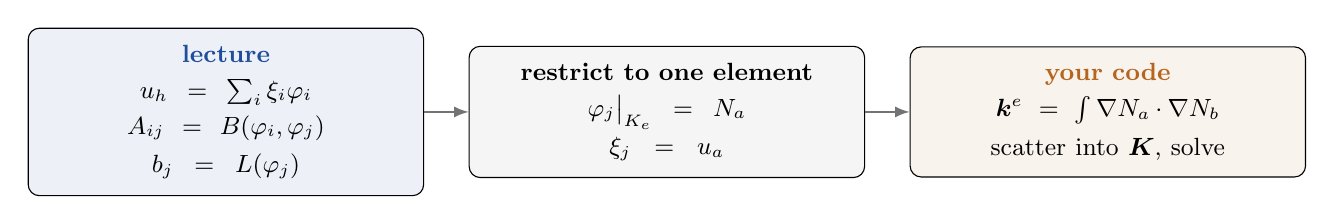
\begin{tikzpicture}[x=1cm,y=1cm,>=latex]
  \node[draw,rounded corners,fill=MathC!8,inner sep=6pt,align=center,text width=4.6cm]
    (A) at (0,0) {\small\mth{\textbf{lecture}}\\[2pt]
      $u_{h}=\sum_{i}\xi_{i}\varphi_{i}$\\[2pt]
      $A_{ij}=B(\varphi_{i},\varphi_{j})$\\[2pt]
      $b_{j}=L(\varphi_{j})$};
  \node[draw,rounded corners,fill=black!4,inner sep=6pt,align=center,text width=4.6cm]
    (B) at (5.6,0) {\small\textbf{restrict to one element}\\[2pt]
      $\varphi_{j}\big|_{K_{e}}=N_{a}$\\[2pt]
      $\xi_{j}=u_{a}$};
  \node[draw,rounded corners,fill=EngC!8,inner sep=6pt,align=center,text width=4.6cm]
    (C) at (11.2,0) {\small\eng{\textbf{your code}}\\[2pt]
      $\bm{k}^{e}=\int\grad N_{a}\!\cdot\!\grad N_{b}$\\[2pt]
      scatter into $\bm{K}$, solve};
  \draw[->,thick,black!55] (A) -- (B);
  \draw[->,thick,black!55] (B) -- (C);
\end{tikzpicture}
\end{center}

\medskip
\noindent\fbox{\parbox{0.955\linewidth}{%
\textbf{The one-sentence answer.} $\varphi$ and $N$ are the same functions:
$\varphi$ is the global view (one per unknown, used to \emph{state} the method
and prove things about it), $N$ is the local view (four per element, used to
\emph{compute}). $\xi_{i}$ and your nodal unknown $u_{i}$ are the same numbers.
The bilinear $N$'s are not an engineering invention bolted on afterwards ---
they are what the lecture's three requirements force on a quadrilateral.}}

\vfill
{\footnotesize\color{black!55}Everything computed, not quoted: the $N_{a}$ in
\eqref{eq:N} were solved from the nodal conditions \eqref{eq:delta}, the
identities \eqref{eq:pou}--\eqref{eq:lin} verified symbolically, and
\eqref{eq:ke}--\eqref{eq:kesq} integrated exactly, with symmetry, zero row sums
and the eigenvalues checked. Script: \texttt{q4\_figs.py} (figures),
and the symbolic work is reproduced in the session log.}

\end{document}
